% !TeX program = xelatex
% Compile: latexmk -xelatex -interaction=nonstopmode -halt-on-error test_loi_giai_mo_rong.tex
\documentclass[11pt,a4paper]{article}
\usepackage{fontspec,polyglossia}
\setdefaultlanguage{vietnamese}
\setmainfont{lmroman10}[Extension=.otf,UprightFont=*-regular,BoldFont=*-bold,ItalicFont=*-italic,BoldItalicFont=*-bolditalic]
\usepackage{amsmath,unicode-math}
\setmathfont{latinmodern-math.otf}
\usepackage[a4paper,margin=2cm,headheight=15pt]{geometry}
\usepackage{booktabs,array,enumitem,xcolor,fancyhdr,graphicx,longtable,hyperref}
\DeclareMathOperator{\MISE}{MISE}
\DeclareMathOperator{\AMISE}{AMISE}
\DeclareMathOperator{\MSE}{MSE}
\DeclareMathOperator{\ISE}{ISE}
\DeclareMathOperator{\IQR}{IQR}
\setcounter{tocdepth}{2}
\allowdisplaybreaks[1]
\hypersetup{colorlinks=true,linkcolor=blue!45!black,pdftitle={Ước lượng mật độ — Bài giảng ôn tập},pdfauthor={}}
\pagestyle{fancy}\fancyhf{}
\fancyhead[L]{\small Thống kê phi tham số — Ước lượng mật độ}
\fancyhead[R]{\small Lời giải từng bước}\fancyfoot[C]{\thepage}
\setlength{\parindent}{0pt}\setlength{\parskip}{4pt}
\setlength{\emergencystretch}{1em}
\setlist{nosep,leftmargin=*}
\newcommand{\E}{\mathbb E}
\newcommand{\R}{\mathbb R}
\newcommand{\fh}{\widehat f_h}
\DeclareMathOperator{\Var}{Var}
\DeclareMathOperator{\Bias}{Bias}
\DeclareMathOperator{\AMSE}{AMSE}
\newcommand{\buoc}[1]{\par\medskip\textbf{#1}\par}
\begin{document}
\begin{center}
{\LARGE\bfseries ƯỚC LƯỢNG MẬT ĐỘ}\\[5pt]
{\Large Bài giảng ôn tập}\\[5pt]
{\normalsize Thống kê phi tham số — Công thức, cách làm và ví dụ}
\end{center}
\pdfbookmark[1]{Bài giảng ngắn: hiểu công thức trước khi làm bài}{intro}

\noindent\textbf{Bổ sung: bộ bài tập trọng tâm Chương 2.}
Mỗi bài trong bộ mới có đề bài, điều kiện, lời giải từng bước, kết luận và lỗi dễ mắc.
\begin{center}
\small
\begin{tabular}{p{.18\textwidth}p{.64\textwidth}r}
\toprule Mã bài & Nội dung (bấm để chuyển tới lời giải) & Trang\\\midrule
1.1--1.5 & \hyperref[ot45:kde-density]{KDE: mật độ hợp lệ, Bias, Variance, AMSE/AMISE, nhân cấp cao} & \pageref{ot45:kde-density}\\
2.1--2.5 & \hyperref[ot45:projection-coeff]{Phép chiếu: hệ số, tương phản, Pythagoras, chọn $D$, histogram} & \pageref{ot45:projection-coeff}\\
2.3(b) & \hyperref[ot45:risk-reformulation]{Tái cấu trúc Bias--Variance và loại hằng số khỏi rủi ro} & \pageref{ot45:risk-reformulation}\\
II.1--II.3 & \hyperref[ot45:constants]{Tính hằng số bốn nhân, KDE trên mẫu nhỏ, hệ số 1.06} & \pageref{ot45:constants}\\
III.1--III.4 & \hyperref[ot45:comparison]{So sánh, chệch biên, oracle/thích ứng và LOOCV} & \pageref{ot45:comparison}\\
\bottomrule
\end{tabular}
\end{center}
\textit{Gợi ý luyện tập 45 phút:} dành 12 phút cho bài tính số, 23 phút cho một bài chứng minh và 10 phút cho lý thuyết/tối ưu hóa. Đây là cách phân bổ thời gian luyện tập, không phải cấu trúc đề thi chính thức.

\section*{1. Ta đang ước lượng điều gì?}
Cho các quan sát $X_1,\ldots,X_n$, ta muốn biết dữ liệu thường tập trung ở đâu. Hàm mật độ $f(x)$ mô tả mức độ tập trung quanh $x$: mật độ cao nghĩa là các khoảng nhỏ quanh đó thường chứa nhiều xác suất hơn.
\[
P(a\leq X\leq b)=\int_a^b f(x)\,dx.
\]
\textbf{Phân biệt:} $f(x)$ là chiều cao của đường mật độ, còn xác suất là diện tích dưới đường đó trên một khoảng. Mật độ có thể lớn hơn 1; điều kiện là $f\geq0$ và tổng diện tích bằng 1. Với phân phối có mật độ, xác suất tại riêng một điểm bằng 0.

\section*{2. KDE: đặt một đường nhân quanh mỗi quan sát}
Thay vì chọn trước một họ phân phối cho $f$, ta đặt quanh mỗi $X_i$ một bản sao của hàm nhân $K$, co giãn theo $h$, rồi lấy trung bình:
\[
\boxed{\widehat f_h(x)=\frac1{nh}\sum_{i=1}^nK\!\left(\frac{x-X_i}{h}\right).}
\]
\begin{itemize}
\item $x$: vị trí muốn tính mật độ; $X_i$: giá trị quan sát thứ $i$; $n$: số quan sát.
\item $K$: hàm quy định hình dạng và trọng số theo khoảng cách. Với nhân không âm có tích phân 1, mỗi bản nhân là một mật độ.
\item $h>0$: băng thông, quyết định độ rộng làm trơn. Đối số $(x-X_i)/h$ đo khoảng cách theo đơn vị $h$.
\end{itemize}
\textbf{Vì sao chia cho $nh$?} Chia cho $n$ để lấy trung bình. Chia thêm cho $h$ để mỗi bản nhân vẫn có diện tích 1 sau khi thay đổi chiều rộng: đặt $u=(x-X_i)/h$ thì $dx=h\,du$, triệt tiêu hệ số $1/h$.

\section*{3. Bài tính số: luôn làm theo bốn bước}
\begin{enumerate}
\item Tính $u_i=(x-X_i)/h$ cho từng quan sát.
\item Kiểm tra miền của nhân: với nhân có giá đỡ $[-1,1]$, đặt $K(u_i)=0$ nếu $|u_i|>1$.
\item Thay từng $u_i$ còn lại vào công thức $K$.
\item Cộng tất cả giá trị nhân rồi chia cho $nh$.
\end{enumerate}
\textbf{Ví dụ một số hạng.} Với $x=3$, $X_i=2$, $h=2$, nhân Epanechnikov:
\[
u_i=\frac{3-2}{2}=\frac12,\qquad
K(u_i)=\frac34\left(1-\frac14\right)=\frac9{16}.
\]
Nếu mẫu có $n=4$ điểm, quan sát này đóng góp $(9/16)/(4\cdot2)=9/128$ vào KDE. Cần cộng đóng góp của \emph{mọi} quan sát mới được đáp số cuối; xem \hyperref[core:calculation]{bài tính Epanechnikov} và Mục \ref{sec:kernels}.

\clearpage
\section*{4. Hai hằng số của nhân dùng để làm gì?}
\[
\mu_2(K)=\int u^2K(u)\,du,\qquad R(K)=\int K(u)^2\,du.
\]
$\mu_2(K)$ là moment bậc hai; với nhân không âm, đối xứng và chuẩn hóa, nó là phương sai của phân phối nhân, biểu thị độ phân tán của nhân. $R(K)$ là tích phân bình phương nhân. Hai hằng số này đưa đặc điểm của $K$ vào công thức sai số.

Tại điểm nội miền giá đỡ, với nhân bậc hai và mật độ đủ trơn, các số hạng xấp xỉ chính là
\[
\underbrace{\E\widehat f_h(x)-f(x)}_{\text{Bias: độ chệch}}
\approx\frac{h^2}{2}\mu_2(K)f''(x),\qquad
\underbrace{\Var\widehat f_h(x)}_{\text{dao động giữa các mẫu}}
\approx\frac{R(K)f(x)}{nh}.
\]
\textbf{Cách hiểu:} nếu lấy mẫu và tính KDE nhiều lần, Bias là khoảng lệch có dấu giữa trung bình các ước lượng và giá trị thật. Variance đo mức dao động của các ước lượng quanh trung bình đó. $f''(x)$ đo độ cong của mật độ; ở đỉnh cong xuống, chệch dẫn đầu thường âm.

\section*{5. Vì sao phải cân bằng Bias và Variance?}
Sai số bình phương trung bình có phân rã chính xác
\[
\MSE(\widehat f_h(x))=\E[(\widehat f_h(x)-f(x))^2]
=\Bias(\widehat f_h(x))^2+\Var\widehat f_h(x).
\]
Thay chệch và phương sai bằng các xấp xỉ ở trên cho
\[
\boxed{\AMSE_x(h)=\frac{h^4}{4}\mu_2(K)^2[f''(x)]^2+\frac{R(K)f(x)}{nh}.}
\]
Trong chế độ xấp xỉ này, tăng $h$ làm bình phương chệch tăng nhưng phương sai giảm. Giảm $h$ thì ngược lại. Để chọn $h$, viết biểu thức thành $Ah^4+B/h$ với $A,B>0$, đạo hàm rồi giải
\[
4Ah^3-\frac{B}{h^2}=0
\quad\Longrightarrow\quad h_* =\left(\frac{B}{4A}\right)^{1/5}.
\]
\textbf{Đừng quên:} bình phương chệch trước khi cộng phương sai. Công thức trên tối ưu sai số tại một điểm; AMISE đánh giá sai số tích phân trên toàn trục và có hệ số khác.

\section*{6. Nhìn yêu cầu đề để chọn cách làm}
\begin{center}
\small
\begin{tabular}{p{.33\textwidth}p{.58\textwidth}}
\toprule
Đề yêu cầu & Bắt đầu từ đâu?\\
\midrule
Tính $\mu_2$, $R(K)$ hoặc KDE & Tích phân theo định nghĩa; lập bảng $u_i,K(u_i)$. Xem \hyperref[core:calculation]{bài tính mẫu}, Mục \ref{sec:kernels}.\\[3pt]
Chứng minh tích phân bằng 1, tính kỳ vọng & Đổi biến để đưa nhân về $K(u)$; ghi cả vi phân và cận. Xem \hyperref[core:expectation]{phần tích phân và kỳ vọng}.\\[3pt]
Chứng minh Bias, Variance & Taylor cho Bias; $\Var Z=\E Z^2-(\E Z)^2$ cho Variance. Xem \hyperref[core:bias]{phần Taylor}, Mục \ref{sec:variance}.\\[3pt]
Tính sai số, tìm $h$ tối ưu & Lập AMSE hoặc AMISE, đạo hàm theo $h$. Xem \hyperref[core:optimal]{bài tối ưu tại điểm}, Mục \ref{sec:amise}.\\[3pt]
Chọn $h$ từ dữ liệu & Quy tắc tham chiếu chuẩn hoặc LOOCV. Xem Mục \ref{sec:silverman}, \ref{sec:cv}.\\
\bottomrule
\end{tabular}
\end{center}
\clearpage
\section*{Đề tổng hợp để tự luyện và các ký hiệu cần hiểu}
Đề dưới đây gồm ba câu. Trong phần giải chi tiết tiếp theo, nội dung được tách thành năm bài độc lập theo chủ đề; mỗi bài nhắc lại đủ dữ kiện và yêu cầu trước khi giải.
Trong toàn bài, $X_1,\ldots,X_n$ là mẫu i.i.d. có mật độ $f$ và
\[
\fh(x)=\frac{1}{nh}\sum_{i=1}^nK\!\left(\frac{x-X_i}{h}\right),
\qquad K(u)=\frac34(1-u^2)\mathbf1_{\{|u|\leq1\}}.
\]
Đặt $\mu_2(K)=\int_{\R}u^2K(u)\,du$ và $R(K)=\int_{\R}K^2(u)\,du$.

\textbf{Câu 1 (3 điểm).} Mẫu $(X_1,X_2,X_3,X_4)=(1,2,4,5)$, $h=2$.
\begin{enumerate}[label=(\alph*)]
\item Tính $\mu_2(K)$ và $R(K)$ (1 điểm).
\item Tính $\fh(3)$ (2 điểm).
\end{enumerate}
\textbf{Câu 2 (3 điểm).} Cho $K$ là nhân đối xứng, $\int K=1$.
\begin{enumerate}[label=(\alph*)]
\item Chứng minh $\int_{\R}\fh(x)\,dx=1$ (1 điểm).
\item Chứng minh $\E\fh(x)=\int K(u)f(x-hu)\,du$ (1 điểm).
\item Giả sử $f\in C^2$, $f''$ bị chặn. Dùng Taylor chứng minh
\[
\E\fh(x)-f(x)=\frac{h^2}{2}\mu_2(K)f''(x)+o(h^2),\qquad h\to0
\]
(1 điểm).
\end{enumerate}
\textbf{Câu 3 (4 điểm).} $f$ là mật độ $\mathcal N(0,1)$, $n=100$, xét tại $x=0$; cho $f(0)\approx0.399$. Dùng Câu 2(c) và
\[
\Var\fh(x)\approx\frac{R(K)f(x)}{nh}.
\]
\begin{enumerate}[label=(\alph*)]
\item Với $h=0.5$, tính chệch, phương sai xấp xỉ và $\AMSE=(\text{chệch})^2+\text{phương sai}$ tại $x=0$ (1.5 điểm).
\item Tìm $h$ tối thiểu hóa $\AMSE(h)$ tại $x=0$ và AMSE tương ứng (2.5 điểm).
\end{enumerate}

\textbf{Đọc ký hiệu.} i.i.d. nghĩa là độc lập và cùng phân phối. $f$ là mật độ thật; $\fh$ là mật độ ước lượng từ mẫu. $x$ là vị trí muốn ước lượng, $X_i$ là quan sát thứ $i$, $n$ là cỡ mẫu, $h>0$ là độ rộng cửa sổ (bandwidth). Hàm chỉ báo $\mathbf1_{\{|u|\leq1\}}$ bằng 1 khi $|u|\leq1$, bằng 0 khi $|u|>1$.

\clearpage
\begingroup
\setlength{\abovedisplayskip}{6pt}
\setlength{\belowdisplayskip}{6pt}
\setlength{\abovedisplayshortskip}{3pt}
\setlength{\belowdisplayshortskip}{3pt}
\renewcommand{\buoc}[1]{\par\textbf{#1}\par}
\section*{Bài 1. Tính hằng số nhân và giá trị KDE}\label{core:calculation}
\textbf{Đề bài.} Cho nhân Epanechnikov
\[
K(u)=\frac34(1-u^2)\mathbf1_{\{|u|\leq1\}},\qquad
\widehat f_h(x)=\frac1{nh}\sum_{i=1}^nK\left(\frac{x-X_i}{h}\right).
\]
\begin{enumerate}[label=(\alph*)]
\item Tính $\mu_2(K)=\int_{\R}u^2K(u)du$ và $R(K)=\int_{\R}K(u)^2du$.
\item Cho mẫu $X=(1,2,4,5)$ và băng thông $h=2$. Tính giá trị mật độ ước lượng $\widehat f_2(3)$.
\end{enumerate}
\textbf{Lời giải.}
\subsection*{(a) Tính hai hằng số của nhân}
\buoc{Bước 1. Xác định miền tích phân và tính đối xứng.}
Vì $K(u)=0$ bên ngoài $[-1,1]$, mọi tích phân có thừa số $K$ chỉ cần tính trên $[-1,1]$. Cả $u^2K(u)$ và $K^2(u)$ đều là hàm chẵn. Dùng
\[
\int_{-1}^1g(u)\,du=2\int_0^1g(u)\,du\quad\text{khi }g(-u)=g(u),
\qquad \int_0^1u^k\,du=\frac{1}{k+1}.
\]
\textit{Tại sao dùng?} Hai công thức này biến tích phân của nhân thành tích phân đa thức đơn giản.

\buoc{Bước 2. Thay $K$ vào định nghĩa của $\mu_2(K)$.}
\begin{align*}
\mu_2(K)&=\frac34\int_{-1}^1u^2(1-u^2)\,du
=\frac32\int_0^1(u^2-u^4)\,du\\
&=\frac32\left[\frac{u^3}{3}-\frac{u^5}{5}\right]_0^1
=\frac32\left(\frac13-\frac15\right)
=\boxed{\frac15}.
\end{align*}
Đây là moment bậc hai của nhân; nó xuất hiện trong \hyperref[core:bias]{bài khai triển độ chệch}.

\buoc{Bước 3. Bình phương toàn bộ $K$ để tính $R(K)$.}
Lưu ý $(3/4)^2=9/16$, $(1-u^2)^2=1-2u^2+u^4$ và chỉ báo bình phương vẫn bằng chính nó. Do đó
\begin{align*}
R(K)&=\frac9{16}\int_{-1}^1(1-2u^2+u^4)\,du
=\frac98\left(1-\frac23+\frac15\right)\\
&=\frac98\cdot\frac8{15}=\boxed{\frac35}.
\end{align*}
$R(K)$ là tích phân bình phương nhân, khác với $\mu_2(K)$; nó xuất hiện trong phương sai xấp xỉ.

\subsection*{(b) Tính $\widehat f_2(3)$}
\buoc{Bước 1. Thay đúng $n=4$, $h=2$, $x=3$.}
\[
\widehat f_2(3)=\frac1{4\cdot2}\sum_{i=1}^4K\!\left(\frac{3-X_i}{2}\right).
\]
\buoc{Bước 2. Tính khoảng cách đã chia cho $h$, rồi tính từng giá trị nhân.}
\begin{center}
\begin{tabular}{cccl}
\toprule
$i$ & $X_i$ & $u_i=(3-X_i)/2$ & $K(u_i)$\\
\midrule
1&1&$1$&$\frac34(1-1)=0$\\
2&2&$1/2$&$\frac34(1-1/4)=9/16$\\
3&4&$-1/2$&$\frac34(1-1/4)=9/16$\\
4&5&$-1$&$\frac34(1-1)=0$\\
\bottomrule
\end{tabular}
\end{center}
\buoc{Bước 3. Cộng rồi nhân với $1/(nh)$.}
\[
\boxed{\widehat f_2(3)=\frac18\left(0+\frac9{16}+\frac9{16}+0\right)
=\frac9{64}=0.140625.}
\]
\textbf{Dễ nhầm:} tại $u=\pm1$, chỉ báo bằng 1 nhưng nhân vẫn bằng 0 vì $1-u^2=0$. Không bỏ hệ số $1/h$ ngoài tổng. Giá trị mật độ tại 3 không phải xác suất $P(X=3)$.
\endgroup

\clearpage
\section*{Bài 2. Tính chuẩn hóa và kỳ vọng của KDE}\label{core:expectation}
\textbf{Đề bài.} Cho $X_1,\ldots,X_n$ độc lập cùng mật độ $f$ bị chặn trên $\R$,
băng thông $h>0$ cố định và nhân $K\geq0$, $\int_{\R}K(u)du=1$. Định nghĩa
\[
\widehat f_h(x)=\frac1{nh}\sum_{i=1}^nK\left(\frac{x-X_i}{h}\right).
\]
\begin{enumerate}[label=(\alph*)]
\item Chứng minh $\widehat f_h(x)\geq0$ và $\int_{\R}\widehat f_h(x)dx=1$ với mọi mẫu.
\item Với $x\in\R$ cố định, chứng minh
$\E\widehat f_h(x)=\int_{\R}K(u)f(x-hu)du$.
\end{enumerate}
\textbf{Lời giải.}
\subsection*{(a) Chứng minh KDE có tổng diện tích bằng 1}
Vì $K\geq0$ và $1/(nh)>0$, ta có ngay $\widehat f_h(x)\geq0$.
\buoc{Bước 1. Đưa tích phân vào tổng hữu hạn.}
Tích phân có tính tuyến tính, vì vậy
\[
\int_{\R}\fh(x)\,dx
=\frac1{nh}\sum_{i=1}^n\int_{\R}K\!\left(\frac{x-X_i}{h}\right)\,dx.
\]
Khi tích phân theo $x$, coi các $X_i$ là những giá trị cố định của mẫu.

\buoc{Bước 2. Đổi biến để bên trong nhân chỉ còn $u$.}
Đặt $u=(x-X_i)/h$. Khi đó $x=X_i+hu$, $dx=h\,du$. Do $h>0$, cận $x=-\infty,+\infty$ tương ứng với $u=-\infty,+\infty$. Suy ra
\[
\int_{\R}K\!\left(\frac{x-X_i}{h}\right)\,dx
=h\int_{\R}K(u)\,du=h.
\]
\textit{Tại sao dùng đổi biến?} Ta biết $\int K(u)\,du=1$; đổi biến đưa tích phân về đúng dạng đã biết đó. Hệ số $h$ sinh ra từ $dx$ sẽ triệt tiêu $1/h$ trong KDE.

\buoc{Bước 3. Có $n$ số hạng đều bằng $h$.}
\[
\boxed{\int_{\R}\fh(x)\,dx=\frac1{nh}\sum_{i=1}^nh
=\frac{nh}{nh}=1.}
\]
Kết quả này đúng với mọi mẫu. Phép tính diện tích chỉ cần $\int K=1$, chưa cần đối xứng. Kết hợp với tính không âm đã chứng minh, $\fh$ là một mật độ.

\subsection*{(b) Tính kỳ vọng của KDE tại một điểm cố định}
\buoc{Bước 1. Dùng tính tuyến tính của kỳ vọng và cùng phân phối.}
Lúc này $x$ cố định còn các $X_i$ là ngẫu nhiên. Vì các $X_i$ cùng phân phối,
\[
\E\fh(x)=\frac1{nh}\sum_{i=1}^n\E K\!\left(\frac{x-X_i}{h}\right)
=\frac1h\E K\!\left(\frac{x-X_1}{h}\right).
\]
\textit{Vì sao $n$ biến mất?} Có $n$ kỳ vọng bằng nhau, nên tổng là $n$ lần một kỳ vọng. Riêng bước này không cần tính độc lập.

\buoc{Bước 2. Viết kỳ vọng bằng tích phân theo mật độ.}
Với $X$ có mật độ $f$, công thức $\E[g(X)]=\int g(t)f(t)\,dt$ cho
\[
\E\fh(x)=\frac1h\int_{-\infty}^{\infty}K\!\left(\frac{x-t}{h}\right)f(t)\,dt.
\]
\buoc{Bước 3. Đổi biến, chú ý dấu âm và cận.}
Đặt $u=(x-t)/h$, suy ra $t=x-hu$, $dt=-h\,du$. Khi $t$ đi từ $-\infty$ đến $+\infty$, $u$ đi từ $+\infty$ đến $-\infty$. Vì thế
\[
\E\fh(x)=\frac1h\int_{+\infty}^{-\infty}K(u)f(x-hu)(-h)\,du
=\boxed{\int_{-\infty}^{\infty}K(u)f(x-hu)\,du}.
\]
Đảo cận loại dấu âm; $h$ triệt tiêu $1/h$. Kỳ vọng KDE là trung bình có trọng số của mật độ quanh $x$, nên thường khác chính $f(x)$: đây là nguồn gốc của độ chệch.

\clearpage
\section*{Bài 3. Khai triển Taylor để tìm độ chệch KDE}\label{core:bias}
\textbf{Đề bài.} Cho $X_1,\ldots,X_n$ độc lập cùng mật độ $f\in C^2(\R)$,
$f''$ bị chặn. Với nhân Epanechnikov
\[
K(u)=\frac34(1-u^2)\mathbf1_{\{|u|\leq1\}},\qquad
\widehat f_h(x)=\frac1{nh}\sum_{i=1}^nK\left(\frac{x-X_i}{h}\right),
\]
đặt $\mu_2(K)=\int_{\R}u^2K(u)du$. Tại $x$ cố định, dùng Taylor chứng minh
\[
\Bias(\widehat f_h(x))=\E\widehat f_h(x)-f(x)
=\frac{h^2}{2}\mu_2(K)f''(x)+o(h^2),\qquad h\to0^+.
\]
Giải thích vì sao số hạng bậc nhất triệt tiêu và tích phân phần dư là $o(h^2)$.

\textbf{Lời giải.} Từ định nghĩa kỳ vọng và phép đổi biến $u=(x-t)/h$, ta có
$\E\widehat f_h(x)=\int_{\R}K(u)f(x-hu)du$.
\textbf{Mục tiêu.} Độ chệch là $\Bias(\fh(x))=\E\fh(x)-f(x)$. Ta cần tìm số hạng chính của hiệu này khi $h\to0^+$, tại $x$ cố định.

\buoc{Bước 1. Khai triển $f(x-hu)$ quanh $x$.}
Taylor bậc hai có dạng $f(x+t)=f(x)+tf'(x)+t^2f''(x)/2+\text{phần dư}$. Thay $t=-hu$:
\[
f(x-hu)=f(x)-hu f'(x)+\frac{h^2u^2}{2}f''(x)+r_h(u).
\]
\textit{Tại sao dùng Taylor?} Công thức kỳ vọng chứa $f(x-hu)$, trong khi độ chệch cần so sánh với $f(x)$. Taylor tách đúng $f(x)$ và các số hạng theo lũy thừa của $h$.

\buoc{Bước 2. Thay vào công thức kỳ vọng rồi tách tích phân.}
\begin{align*}
\E\fh(x)
&=f(x)\int K(u)\,du-hf'(x)\int uK(u)\,du\\
&\quad+\frac{h^2}{2}f''(x)\int u^2K(u)\,du+\int K(u)r_h(u)\,du.
\end{align*}
Các đại lượng $f(x),f'(x),f''(x),h$ không phụ thuộc $u$ nên được đưa ra ngoài tích phân.

\buoc{Bước 3. Dùng chuẩn hóa và đối xứng của nhân.}
\[
\int K(u)\,du=1,\qquad \int uK(u)\,du=0,\qquad
\int u^2K(u)\,du=\mu_2(K).
\]
Tích phân giữa bằng 0 vì $K(-u)=K(u)$ nên $uK(u)$ là hàm lẻ: phần âm và phần dương triệt tiêu. Đây chính là bước sử dụng giả thiết đối xứng để loại số hạng bậc $h$.

\buoc{Bước 4. Giải thích vì sao tích phân phần dư là $o(h^2)$.}
Đối với nhân Epanechnikov của đề, chỉ cần xét $|u|\leq1$. Dạng phần dư tích phân của Taylor cho
\[
r_h(u)=h^2u^2\int_0^1(1-s)\{f''(x-shu)-f''(x)\}\,ds.
\]
Đặt $\omega_x(h)=\sup_{|v-x|\leq h}|f''(v)-f''(x)|$. Do $f''$ liên tục tại $x$, $\omega_x(h)\to0$. Với $|u|\leq1$,
\[
|r_h(u)|\leq\frac{h^2u^2}{2}\omega_x(h),\qquad
\left|\int K(u)r_h(u)\,du\right|
\leq\frac{h^2}{2}\omega_x(h)\mu_2(K)=o(h^2).
\]
Ký hiệu $o(h^2)$ nghĩa là phần dư chia cho $h^2$ tiến về 0. Bước này bảo đảm rằng phần dư vẫn nhỏ sau khi lấy tích phân.

\buoc{Bước 5. Trừ $f(x)$ và kết luận.}
\[
\boxed{\E\fh(x)-f(x)=\frac{h^2}{2}\mu_2(K)f''(x)+o(h^2).}
\]
Riêng Epanechnikov: $\Bias(\fh(x))=h^2f''(x)/10+o(h^2)$.

\textbf{Lưu ý về giả thiết tổng quát.} Nếu thay Epanechnikov bằng nhân đối xứng bất kỳ, chứng minh còn cần moment tuyệt đối bậc hai hữu hạn: $\int u^2|K(u)|\,du<\infty$. Khi đó $f''$ bị chặn giúp áp dụng định lý hội tụ bị trội cho phần dư chia $h^2$. Nhân của đề tự động thỏa điều kiện moment vì bị chặn và bằng 0 ngoài $[-1,1]$.

\clearpage
\section*{Bài 4. Tính chệch, phương sai và AMSE tại một điểm}
\textbf{Đề bài.} Cho mẫu độc lập $X_1,\ldots,X_{100}$ từ mật độ chuẩn tắc
$f(x)=(2\pi)^{-1/2}e^{-x^2/2}$. Xét KDE
\[
\widehat f_h(x)=\frac1{100h}\sum_{i=1}^{100}K\left(\frac{x-X_i}{h}\right),\qquad
K(u)=\frac34(1-u^2)\mathbf1_{\{|u|\leq1\}}.
\]
Cho $\mu_2(K)=1/5$, $R(K)=3/5$, $f(0)\approx0.399$ và các công thức xấp xỉ
\[
\Bias(\widehat f_h(x))\approx\frac{h^2}{2}\mu_2(K)f''(x),\qquad
\Var(\widehat f_h(x))\approx\frac{R(K)f(x)}{100h}.
\]
Với $h=0.5$, tính $f''(0)$, chệch, phương sai và
$\AMSE=(\text{chệch xấp xỉ})^2+\text{phương sai xấp xỉ}$ tại $x=0$.
Giữ giá trị $f(0)=0.399$ khi thay số để các đáp số nhất quán.

\textbf{Lời giải.}
\buoc{Bước 1. Tính $f''(0)$ từ mật độ chuẩn tắc.}
Ta biết
\[
f(x)=\frac1{\sqrt{2\pi}}e^{-x^2/2}.
\]
Đạo hàm hàm hợp: $(e^{g(x)})'=g'(x)e^{g(x)}$, với $g'(x)=-x$. Do đó $f'(x)=-xf(x)$. Tiếp tục dùng đạo hàm tích:
\[
f''(x)=(-x)'f(x)+(-x)f'(x)
=-f(x)+x^2f(x)=(x^2-1)f(x).
\]
Tại $x=0$,
\[
\boxed{f''(0)=-f(0)\approx-0.399.}
\]
\textit{Tại sao phải tính?} Công thức chệch phụ thuộc đạo hàm bậc hai của mật độ, không phải đạo hàm bậc nhất. Đỉnh của mật độ chuẩn cong xuống nên $f''(0)<0$.

\buoc{Bước 2. Tính chệch xấp xỉ.}
Lấy số hạng chính trong khai triển chệch, bỏ phần dư $o(h^2)$:
\begin{align*}
\Bias(\fh(0))&\approx\frac{h^2}{2}\mu_2(K)f''(0)\\
&=\frac{(0.5)^2}{2}\cdot\frac15\cdot(-0.399)
=\boxed{-0.009975}.
\end{align*}
Độ chệch âm nghĩa là trung bình qua các mẫu, ước lượng tại đỉnh thấp hơn mật độ thật. Đây là hiệu ứng làm trơn đỉnh, không phải mật độ ước lượng âm.

\buoc{Bước 3. Tính phương sai xấp xỉ theo công thức đề cho.}
\[
\Var\fh(0)\approx\frac{R(K)f(0)}{nh}
=\frac{(3/5)\cdot0.399}{100\cdot0.5}
=\frac{0.2394}{50}=\boxed{0.004788}.
\]
\textit{Ý nghĩa:} phương sai đo mức dao động của $\fh(0)$ nếu lấy lại mẫu nhiều lần. Nó khác phương sai của một biến ngẫu nhiên có mật độ $f$, và cũng khác độ lệch chuẩn (căn bậc hai của phương sai).

\buoc{Bước 4. Bình phương chệch trước khi cộng phương sai.}
Với một ước lượng $T$ của $\theta$, ta có
\[
\E[(T-\theta)^2]=\Var(T)+(\E T-\theta)^2.
\]
Công thức này có được bằng cách viết $T-\theta=(T-\E T)+(\E T-\theta)$ rồi khai triển bình phương; số hạng chéo có kỳ vọng 0. Khi dùng các biểu thức xấp xỉ của chệch và phương sai, ta được AMSE:
\begin{align*}
\AMSE(0.5)&=(-0.009975)^2+0.004788\\
&=0.000099500625+0.004788\\
&=\boxed{0.004887500625\approx0.00488750}.
\end{align*}
\textbf{Dễ nhầm:} không cộng trực tiếp chệch âm vào phương sai; phải dùng \emph{bình phương} chệch. Các kết quả số dùng $f(0)=0.399$ theo giá trị làm tròn đề cho. AMSE là xấp xỉ của MSE, không phải MSE chính xác ở mẫu hữu hạn.

\clearpage
\section*{Bài 5. Chọn băng thông tối thiểu hóa AMSE}\label{core:optimal}
\textbf{Đề bài.} Cho $X_1,\ldots,X_{100}$ độc lập từ mật độ $f$ chuẩn tắc.
Ước lượng $f(0)$ bằng KDE với nhân Epanechnikov và băng thông $h>0$.
Cho $\mu_2(K)=1/5$, $R(K)=3/5$, $f(0)\approx0.399$, $f''(0)\approx-0.399$.
Xét hàm sai số xấp xỉ
\[
\AMSE(h)=\frac{h^4}{4}\mu_2(K)^2[f''(0)]^2+\frac{R(K)f(0)}{100h}.
\]
\begin{enumerate}[label=(\alph*)]
\item Viết AMSE thành $Ah^4+B/h$ và xác định $A,B$.
\item Tìm $h_*>0$ làm AMSE nhỏ nhất; chứng minh đó là cực tiểu toàn cục duy nhất.
\item Tính AMSE nhỏ nhất và tỷ số giữa phương sai xấp xỉ với bình phương chệch tại $h_*$.
\end{enumerate}
\textbf{Lời giải.}
\buoc{Bước 1. Giữ $h$ là biến, thay các hằng số đã biết.}
\[
\Bias(\fh(0))\approx-0.0399h^2,\qquad
\Var\fh(0)\approx\frac{0.002394}{h}.
\]
Vì vậy, với $h>0$,
\[
\boxed{\AMSE(h)=Ah^4+\frac Bh,\qquad
A=(0.0399)^2=0.00159201,\quad B=0.002394.}
\]
\textit{Tại sao có $h^4$?} Chệch tỷ lệ với $h^2$, nên bình phương chệch tỷ lệ với $(h^2)^2=h^4$. Khi $h$ tăng, bình phương chệch tăng còn phương sai giảm; cần cân bằng hai phần này.

\buoc{Bước 2. Đạo hàm và giải phương trình bằng 0.}
Vì $(h^4)'=4h^3$ và $(h^{-1})'=-h^{-2}$,
\[
\AMSE'(h)=4Ah^3-\frac{B}{h^2}=0
\quad\Longleftrightarrow\quad4Ah^5=B.
\]
Ta nhân hai vế với $h^2>0$, rồi lấy căn bậc năm:
\[
h_* =\left(\frac{B}{4A}\right)^{1/5}
=\left(\frac{0.002394}{4\cdot0.00159201}\right)^{1/5}
=\boxed{0.82228747\approx0.8223}.
\]
Để bấm máy: tính $0.002394/(4\times0.00159201)$ trước, rồi nâng kết quả lên lũy thừa $1/5=0.2$.

\buoc{Bước 3. Kiểm tra nghiệm thực sự là điểm cực tiểu toàn cục.}
\[
\AMSE''(h)=12Ah^2+\frac{2B}{h^3}>0\qquad(h>0).
\]
Do $A,B>0$, hàm lồi nghiêm ngặt; đồng thời $\AMSE(h)\to\infty$ khi $h\to0^+$ hoặc $h\to\infty$. Vì vậy nghiệm trên là điểm tối thiểu duy nhất trên $h>0$.

\buoc{Bước 4. Thay $h_*$ vào AMSE.}
\begin{align*}
A h_*^4&\approx0.000727847647,\\
B/h_*&\approx0.002911390586,\\
\AMSE(h_*)&\approx0.000727847647+0.002911390586
=\boxed{0.003639238233\approx0.00363924}.
\end{align*}
\textbf{Cách kiểm tra nhanh:} từ $4Ah_*^5=B$, suy ra $B/h_*=4Ah_*^4$. Tại nghiệm tối ưu, phương sai xấp xỉ bằng 4 lần bình phương chệch, và $\AMSE(h_*)=5Ah_*^4$. Hai thành phần không cần bằng nhau.

\textbf{Công thức tổng quát rút ra từ phép tính:}
\[
\AMSE_x(h)=\frac{\mu_2(K)^2[f''(x)]^2}{4}h^4+\frac{R(K)f(x)}{nh},
\qquad
h_*(x)=\left[\frac{R(K)f(x)}{n\mu_2(K)^2[f''(x)]^2}\right]^{1/5}.
\]
Công thức áp dụng ở điểm có $f(x)>0$, $f''(x)\ne0$ và $\mu_2(K)\ne0$. Đây là tối ưu \emph{AMSE tại $x=0$}; không phải tối ưu sai số tích phân trên toàn trục, cũng không khẳng định tối ưu MSE chính xác.

\clearpage
\section*{Bản trình bày ngắn để ôn tập}
Sau khi hiểu các bước phía trước, có thể rút lời giải thành các dòng sau.

\textbf{Bài 1(a) — Hằng số nhân Epanechnikov.} Vì nhân bằng 0 ngoài $[-1,1]$ và các hàm dưới dấu tích phân là chẵn,
\[
\mu_2(K)=\frac32\left(\frac13-\frac15\right)=\frac15,
\qquad R(K)=\frac98\left(1-\frac23+\frac15\right)=\frac35.
\]
\textbf{Bài 1(b) — KDE với mẫu $(1,2,4,5)$, $h=2$, tại $x=3$.} Các đối số nhân là $1,1/2,-1/2,-1$, nên
\[
\widehat f_2(3)=\frac18\left(0+\frac9{16}+\frac9{16}+0\right)=\frac9{64}.
\]
\textbf{Bài 2(a) — Chuẩn hóa KDE.} Đổi biến $u=(x-X_i)/h$, $dx=h\,du$:
\[
\int\fh(x)\,dx=\frac1{nh}\sum_{i=1}^nh\int K(u)\,du=1.
\]
\textbf{Bài 2(b) — Kỳ vọng KDE.} Cùng phân phối và tuyến tính của kỳ vọng cho
\[
\E\fh(x)=\frac1h\int K\!\left(\frac{x-t}{h}\right)f(t)\,dt
=\int K(u)f(x-hu)\,du,
\]
trong đó đổi biến $t=x-hu$, $dt=-h\,du$ và đảo cận.

\textbf{Bài 3 — Chệch của KDE Epanechnikov.} Với $|u|\leq1$, Taylor cho
\[
f(x-hu)=f(x)-hu f'(x)+\frac{h^2u^2}{2}f''(x)+r_h(u),
\]
với $|r_h(u)|\leq h^2u^2\omega_x(h)/2$, $\omega_x(h)\to0$ do $f''$ liên tục. Vì $\int K=1$, $\int uK=0$ và $\int u^2K=\mu_2(K)$,
\[
\E\fh(x)-f(x)=\frac{h^2}{2}\mu_2(K)f''(x)+o(h^2).
\]
\textbf{Bài 4 — AMSE tại 0, mẫu chuẩn tắc, $n=100$.} $f'(x)=-xf(x)$, $f''(x)=(x^2-1)f(x)$, nên $f''(0)\approx-0.399$. Với $h=0.5$,
\[
\Bias\approx\frac{0.5^2}{2}\cdot\frac15\cdot(-0.399)=-0.009975,
\qquad \Var\approx\frac{(3/5)\cdot0.399}{100\cdot0.5}=0.004788.
\]
Suy ra $\AMSE(0.5)=(-0.009975)^2+0.004788\approx0.00488750$.

\textbf{Bài 5 — Băng thông tối ưu tại 0.} $\AMSE(h)=0.00159201h^4+0.002394/h$, với $h>0$.
\[
\AMSE'(h)=4(0.00159201)h^3-0.002394h^{-2}=0
\ \Longrightarrow\ 
h_* =\left[\frac{0.002394}{4(0.00159201)}\right]^{1/5}\approx0.8223.
\]
Vì $\AMSE''(h)>0$ với mọi $h>0$, đây là điểm tối thiểu duy nhất, và
\[
\boxed{\AMSE(h_*)\approx0.00363924.}
\]
\vfill
\textbf{Bốn điều tự kiểm tra:} có hệ số $1/(nh)$ trong KDE; đổi biến có vi phân và cận mới; đối xứng làm moment bậc nhất bằng 0; AMSE cộng \emph{bình phương} chệch với phương sai.

\clearpage
\section*{Các chủ đề ôn tập}
\textbf{Mục tiêu.} Không chỉ nhớ đáp số: nhận diện dạng bài, chọn công thức, kiểm tra điều kiện, thay số và tự phát hiện lỗi. Mỗi mục có bài mẫu hoặc phép suy luận đủ để tự làm lại.

\textbf{Bốn mục ôn tập trọng tâm:} nhân Uniform và Triangular (Mục \ref{sec:kernels}); chứng minh phương sai (Mục \ref{sec:variance}); quy tắc tham chiếu chuẩn (Mục \ref{sec:silverman}); LOOCV (Mục \ref{sec:cv}). Sau đó học AMISE, nhân cấp cao, chệch biên và các phương pháp liên quan. Các phần bao quát Chương 2 gồm Histogram và CV (Mục \ref{sec:hist-detail}, \ref{sec:hist-cv}), phép chiếu (Mục \ref{sec:projection}), Root--Unroot (Mục \ref{sec:root}) và KDE đa chiều (Mục \ref{sec:multivariate}).

\textbf{Quy ước chung.} $h>0$, mẫu i.i.d., tích phân không ghi cận là trên $\R$; $K_h(t)=h^{-1}K(t/h)$. Đặt $\mu_j(K)=\int u^jK(u)du$ và $R(g)=\int g^2$. Khi viết công thức tiệm cận, $h=h_n\to0$, thường kèm $nh_n\to\infty$. Các ví dụ số dùng định nghĩa nhân trong đề, không tự chuẩn hóa phương sai của nhân về 1.

\textbf{Bốn điểm cần đọc chính xác.}
\begin{enumerate}
\item AMISE là \emph{xấp xỉ tiệm cận} của MISE. Hai đại lượng không đồng nhất ở mẫu hữu hạn.
\item EDF không có đạo hàm cổ điển tại điểm nhảy; không viết đạo hàm ở đó ``bằng $\infty$'' như một giá trị đạo hàm thông thường.
\item Hệ số $1.06$ đến từ tối ưu AMISE dưới mô hình chuẩn; quy tắc Silverman bền vững thường dùng hệ số $0.9$. Phải ghi rõ phiên bản sử dụng.
\item Nhân ``cấp $\ell$'' có hai quy ước đánh số khác nhau. Ta sẽ so sánh trực tiếp bằng các moment triệt tiêu.
\end{enumerate}
\begingroup
\small
\tableofcontents
\endgroup
\setlength{\abovedisplayskip}{8pt}
\setlength{\belowdisplayskip}{8pt}
\setlength{\abovedisplayshortskip}{3pt}
\setlength{\belowdisplayshortskip}{4pt}
\renewcommand{\buoc}[1]{\par\smallskip\textbf{#1}\par\nopagebreak[4]}

\clearpage
\section{Nhóm 1: Tính số với các nhân và tối ưu AMISE}
\subsection{Uniform, Triangular, Gaussian: hằng số và KDE [ưu tiên]}\label{sec:kernels}
\textbf{Đề bài.} Với mẫu $X=(1,2,4,5)$, $n=4$, $h=2$, xét
$\widehat f_h(x)=(nh)^{-1}\sum_iK((x-X_i)/h)$.
Lần lượt dùng ba nhân
\[
K_U(u)=\tfrac12\mathbf1_{\{|u|\leq1\}},\quad
K_T(u)=(1-|u|)\mathbf1_{\{|u|\leq1\}},\quad
K_G(u)=\frac{e^{-u^2/2}}{\sqrt{2\pi}}.
\]
Với mỗi nhân, tính $\mu_2(K)=\int_{\R}u^2K(u)du$, $R(K)=\int_{\R}K(u)^2du$
và giá trị mật độ ước lượng $\widehat f_2(3)$.

\textbf{Lời giải.}

\buoc{Bước chung: tách phần phụ thuộc nhân khỏi phần phụ thuộc mẫu.}
Với mọi nhân, $n=4$ và các đối số đều là
\[
(u_1,u_2,u_3,u_4)=\left(\frac{3-1}{2},\frac{3-2}{2},\frac{3-4}{2},\frac{3-5}{2}\right)
=(1,1/2,-1/2,-1).
\]
Do đó $\widehat f_2(3)=\{K(1)+K(1/2)+K(-1/2)+K(-1)\}/8$. Chỉ cần đổi công thức $K$, không đổi hệ số $1/(nh)$.

\subsubsection*{A. Nhân Uniform: $K(u)=\tfrac12\mathbf1_{\{|u|\leq1\}}$}
\buoc{Bước 1. Kiểm tra chuẩn hóa.}
$\int K=(1/2)\times2=1$. Hình chữ nhật có chiều rộng 2 và chiều cao $1/2$ nên diện tích là 1.
\buoc{Bước 2. Tính moment bậc hai từ định nghĩa.}
\[
\mu_2(K)=\frac12\int_{-1}^1u^2du
=\int_0^1u^2du=\left[\frac{u^3}{3}\right]_0^1=\boxed{\frac13}.
\]
\buoc{Bước 3. Tính tích phân bình phương nhân.}
\[
R(K)=\int_{-1}^1\left(\frac12\right)^2du=\frac14\times2=\boxed{\frac12}.
\]
\buoc{Bước 4. Tính KDE bằng đếm điểm trong cửa sổ.}
Cả bốn đối số thỏa $|u_i|\leq1$, kể cả $u_i=\pm1$, nên
\[
\boxed{\widehat f_2(3)=\frac18\cdot4\cdot\frac12=\frac14=0.25.}
\]
Tổng quát $\widehat f_h(x)=N_x/(2nh)$, với $N_x=\#\{i:|x-X_i|\leq h\}$. Công thức này chỉ đúng cho nhân Uniform đúng chuẩn hóa đang dùng.

\subsubsection*{B. Nhân Triangular: $K(u)=(1-|u|)\mathbf1_{\{|u|\leq1\}}$}
\buoc{Bước 1. Dùng đối xứng để bỏ dấu giá trị tuyệt đối.}
Trên $[0,1]$, $|u|=u$. Chuẩn hóa: $\int K=2\int_0^1(1-u)du=1$.
\buoc{Bước 2. Tính hai tích phân.}
\begin{align*}
\mu_2(K)&=2\int_0^1u^2(1-u)du
=2\left(\frac13-\frac14\right)=\boxed{\frac16},\\
R(K)&=2\int_0^1(1-u)^2du
=2\left(1-1+\frac13\right)=\boxed{\frac23}.
\end{align*}
\buoc{Bước 3. Tính trọng số của từng điểm.}
$K(\pm1)=0$, $K(\pm1/2)=1/2$, nên
\[
\boxed{\widehat f_2(3)=\frac18(0+1/2+1/2+0)=\frac18=0.125.}
\]
\textbf{Điểm cần nhớ:} cùng ở đầu mút $|u|=1$, Uniform cho trọng số $1/2$, còn Triangular và Epanechnikov cho 0.

\subsubsection*{C. Nhân Gaussian: $K(u)=\phi(u)=(2\pi)^{-1/2}e^{-u^2/2}$}
\buoc{Bước 1. Nhận diện moment của chuẩn tắc.}
Vì $\phi$ là mật độ của $Z\sim\mathcal N(0,1)$,
\[
\mu_2(K)=\E Z^2=\Var Z+(\E Z)^2=1+0=\boxed{1}.
\]
Có thể kiểm tra bằng tích phân từng phần: $\phi'(u)=-u\phi(u)$, nên
$\int u^2\phi(u)du=-[u\phi(u)]_{-\infty}^{\infty}+\int\phi(u)du=1$.
\buoc{Bước 2. Bình phương mật độ rồi dùng tích phân Gaussian.}
\[
R(K)=\frac1{2\pi}\int e^{-u^2}du
=\frac{\sqrt\pi}{2\pi}=\boxed{\frac1{2\sqrt\pi}\approx0.282095}.
\]
Công thức $\int e^{-u^2}du=\sqrt\pi$ trên toàn trục được suy ra từ chuẩn hóa của phân phối chuẩn và phép đổi biến $z=\sqrt2u$.
\buoc{Bước 3. Tính KDE; không ngắt ở $|u|=1$.}
\[
\widehat f_2(3)=\frac{2\phi(1)+2\phi(1/2)}8
=\frac{0.241970725+0.352065327}{4}
=\boxed{0.148509013}.
\]
Gaussian có giá đỡ toàn trục: quan sát xa vẫn góp trọng số dương, dù có thể rất nhỏ.

\subsubsection*{Bảng đối chiếu để kiểm tra kết quả}
\begin{center}
\begin{tabular}{lccc}
\toprule
Nhân & $\mu_2(K)$ & $R(K)$ & $\widehat f_2(3)$\\
\midrule
Uniform & $1/3$ & $1/2$ & $1/4$\\
Triangular & $1/6$ & $2/3$ & $1/8$\\
Epanechnikov & $1/5$ & $3/5$ & $9/64$\\
Gaussian & $1$ & $1/(2\sqrt\pi)$ & $0.148509013$\\
\bottomrule
\end{tabular}
\end{center}
Không so sánh chất lượng nhân chỉ bằng $R(K)$: độ chệch còn chứa $\mu_2(K)$, và cùng giá trị $h$ chưa tạo cùng độ rộng làm trơn thực tế. Độ lệch chuẩn của nhân đã co giãn là $h\sqrt{\mu_2(K)}$.

\subsection{Đổi điểm tính, đổi cửa sổ và kiểm tra chỉ báo}
\textbf{Đề bài.} Cho $X=(1,2,4,5)$, $n=4$ và
$\widehat f_h(x)=(4h)^{-1}\sum_{i=1}^4K((x-X_i)/h)$.
Tính KDE tại $x=1.5$ và $x=4.5$ với từng $h\in\{1,1.5\}$, lần lượt dùng
Uniform $K(u)=\frac12\mathbf1_{\{|u|\leq1\}}$,
Triangular $K(u)=(1-|u|)\mathbf1_{\{|u|\leq1\}}$,
Epanechnikov $K(u)=\frac34(1-u^2)\mathbf1_{\{|u|\leq1\}}$
và Gaussian $K(u)=(2\pi)^{-1/2}e^{-u^2/2}$.
Giải thích vì sao các nhân compact bỏ một số quan sát còn Gaussian giữ tất cả.

\textbf{Lời giải.}
\buoc{Bước 1. Lập đối số trước khi tính nhân.}
\begin{center}
\begin{tabular}{ccrrrr}
\toprule
$x$&$h$&$u_1$&$u_2$&$u_3$&$u_4$\\
\midrule
$1.5$&$1$&$1/2$&$-1/2$&$-5/2$&$-7/2$\\
$1.5$&$1.5$&$1/3$&$-1/3$&$-5/3$&$-7/3$\\
$4.5$&$1$&$7/2$&$5/2$&$1/2$&$-1/2$\\
$4.5$&$1.5$&$7/3$&$5/3$&$1/3$&$-1/3$\\
\bottomrule
\end{tabular}
\end{center}
Với ba nhân giá đỡ $[-1,1]$, chỉ hai điểm gần nhất được giữ. Mẫu đối xứng quanh 3 và các nhân đối xứng, nên kết quả tại $1.5$ và $4.5$ giống nhau khi dùng cùng $h$.

\buoc{Bước 2. Ví dụ chi tiết cho Epanechnikov.}
Khi $x=1.5,h=1$: $K(\pm1/2)=\frac34(1-1/4)=9/16$, còn hai giá trị kia bằng 0. Do đó
\[
\widehat f_1(1.5)=\frac14\left(\frac9{16}+\frac9{16}\right)=\boxed{\frac9{32}}.
\]
Khi $h=1.5$: $K(\pm1/3)=\frac34(1-1/9)=2/3$, hệ số ngoài tổng là $1/(4\cdot1.5)=1/6$. Vì vậy
\[
\widehat f_{1.5}(1.5)=\frac16\left(\frac23+\frac23\right)=\boxed{\frac29}.
\]
\buoc{Bước 3. Lặp lại với các nhân khác.}
\begin{center}
\begin{tabular}{lcc}
\toprule
Nhân & $h=1$, $x=1.5$ hoặc $4.5$ & $h=1.5$, $x=1.5$ hoặc $4.5$\\
\midrule
Uniform & $(1/4)(1/2+1/2)=1/4$ & $(1/6)(1/2+1/2)=1/6$\\
Triangular & $(1/4)(1/2+1/2)=1/4$ & $(1/6)(2/3+2/3)=2/9$\\
Epanechnikov & $9/32$ & $2/9$\\
\bottomrule
\end{tabular}
\end{center}
Gaussian vẫn giữ cả bốn quan sát. Chẳng hạn
\[
\widehat f_1(1.5)=\frac{2\phi(1/2)+\phi(5/2)+\phi(7/2)}4
\approx0.18063291.
\]
Với $h=1.5$, giá trị là $\{2\phi(1/3)+\phi(5/3)+\phi(7/3)\}/6\approx0.14674425$.

\buoc{Phân biệt hai khái niệm ``biên''.}
$1.5$ và $4.5$ là các vị trí gần hai đầu của \emph{mẫu} này; chưa biết miền giá đỡ của $f$ thì chưa thể gọi chúng là biên thật của phân phối. Chệch biên ở Nhóm 2 nói về biên miền giá đỡ, ví dụ $f(x)=0$ với $x<0$.

\textbf{Bài tự kiểm tra.} Uniform, $x=3,h=1$: chỉ $X=2,4$ nằm trong cửa sổ đóng $[2,4]$, nên $\widehat f_1(3)=2/(2\cdot4\cdot1)=1/4$. Với Triangular hoặc Epanechnikov, hai điểm này nằm đúng nơi nhân bằng 0, nên KDE bằng 0. Quy ước $\leq$ hay $<$ ảnh hưởng bài tính Uniform ở đầu mút, dù không ảnh hưởng tích phân.

\subsection{Từ AMSE tại một điểm sang AMISE trên toàn trục}\label{sec:amise}
\textbf{Đề bài.} Cho mẫu $n$ quan sát độc lập từ mật độ $f$ của
$\mathcal N(0,\sigma^2)$, $\sigma>0$, và KDE
$\widehat f_h(x)=(nh)^{-1}\sum_iK((x-X_i)/h)$.
Nhân $K$ đối xứng, chuẩn hóa, có $\mu_2(K)\ne0$ và $R(K)<\infty$.
Với $R(f'')=\int_{\R}f''(x)^2dx$, dùng
\[
\AMISE(h)=\tfrac14\mu_2(K)^2R(f'')h^4+\frac{R(K)}{nh}
\]
để tìm $h_*$, giá trị AMISE nhỏ nhất và tốc độ theo $n$.
Sau đó thay $R(f'')=3/(8\sqrt\pi\sigma^5)$ để tính các hằng số cho những nhân trong bảng lời giải.

\textbf{Lời giải.}
\buoc{Bước 1. Phân biệt đại lượng chính xác và xấp xỉ.}
\[
\MISE(h)=\E\int(\fh(x)-f(x))^2dx
=\int\Bias(\fh(x))^2dx+\int\Var\fh(x)dx.
\]
Dưới điều kiện trơn và khả tích bảo đảm khai triển theo chuẩn $L^2$, các số hạng dẫn đầu là
\[
\boxed{\AMISE(h)=\frac{h^4}{4}\mu_2(K)^2R(f'')+\frac{R(K)}{nh}.}
\]
Số hạng thứ hai dùng $\int f(x)dx=1$. Không thay bằng $f(0)$: đó là công thức AMSE tại 0, không phải công thức toàn cục. Chỉ có khai triển tại từng điểm thì chưa đủ để tự ý tích phân phần dư trên toàn $\R$.

\buoc{Bước 2. Lấy đạo hàm theo $h$.}
Viết $A=\mu_2(K)^2R(f'')/4$ và $B=R(K)/n$; giả sử $A,B>0$.
\[
\AMISE'(h)=4Ah^3-Bh^{-2}=0
\Longrightarrow
\boxed{h_* =\left[\frac{R(K)}{n\mu_2(K)^2R(f'')}\right]^{1/5}.}
\]
Vì $12Ah^2+2B/h^3>0$, đây là điểm tối thiểu duy nhất. Tại đó,
\[
\boxed{\AMISE(h_*)=\frac54\big\{\mu_2(K)^2R(f'')\big\}^{1/5}
\left\{\frac{R(K)}n\right\}^{4/5}.}
\]
Cách suy ra: từ $B/h_*=4Ah_*^4$, tổng hai thành phần bằng $5Ah_*^4$.

\buoc{Bước 3. Thay $R(f'')=3/(8\sqrt\pi\sigma^5)$.}
\[
\boxed{h_* =\left[\frac{8\sqrt\pi R(K)}{3\mu_2(K)^2}\right]^{1/5}\sigma n^{-1/5}.}
\]
\begin{center}
\begin{tabular}{lcc}
\toprule
Nhân & $h_*/(\sigma n^{-1/5})$ dạng chính xác & Xấp xỉ\\
\midrule
Uniform & $(12\sqrt\pi)^{1/5}$ & $1.8431$\\
Triangular & $(64\sqrt\pi)^{1/5}$ & $2.5760$\\
Epanechnikov & $(40\sqrt\pi)^{1/5}$ & $2.3449$\\
Gaussian & $(4/3)^{1/5}$ & $1.0592$\\
\bottomrule
\end{tabular}
\end{center}
Các hệ số khác nhau do cách co giãn nhân; không có nghĩa Gaussian luôn dùng cửa sổ hiệu dụng nhỏ hơn mọi nhân khác.

\buoc{Bước 4. Ví dụ số đối chiếu đề gốc.}
Với Epanechnikov, $n=100,\sigma=1$, $h_{*,\mathrm{AMISE}}=(40\sqrt\pi/100)^{1/5}\approx0.9335$ và $\AMISE(h_*)\approx0.008034$. Khác $h_{*,\mathrm{AMSE}(0)}\approx0.8223$ ở đề gốc vì hai hàm mục tiêu khác nhau. Không so sánh trực tiếp hai giá trị sai số để kết luận một cách chọn tốt hơn.

\subsubsection*{Nếu đề yêu cầu tự chứng minh $R(f'')$ của chuẩn}
Với $z=x/\sigma$, $f(x)=\phi(z)/\sigma$ và $f''(x)=\sigma^{-3}(z^2-1)\phi(z)$. Do $dx=\sigma dz$,
\[
R(f'')=\frac{1}{2\pi\sigma^5}\int(z^4-2z^2+1)e^{-z^2}dz.
\]
Đặt $I_{2k}=\int z^{2k}e^{-z^2}dz$. Tích phân từng phần cho
$I_{2k}=\frac{2k-1}{2}I_{2k-2}$, với $I_0=\sqrt\pi$; do đó $I_2=\sqrt\pi/2$, $I_4=3\sqrt\pi/4$. Thay vào:
\[
R(f'')=\frac{1}{2\pi\sigma^5}\left(\frac34-1+1\right)\sqrt\pi
=\boxed{\frac3{8\sqrt\pi\sigma^5}}.
\]
\textbf{Mẹo kiểm tra đơn vị:} $R(f'')$ tỷ lệ $\sigma^{-5}$, nên căn bậc năm trong $h_*$ phải đưa về một đại lượng tỷ lệ với $\sigma$.

\section{Nhóm 2: Phương sai, nhân cấp cao và chệch biên}
\subsection{Chứng minh phương sai tiệm cận [ưu tiên]}\label{sec:variance}
\textbf{Đề bài.} Cho $X_1,\ldots,X_n$ độc lập cùng mật độ $f$ và
$\widehat f_h(x)=(nh)^{-1}\sum_iK((x-X_i)/h)$.
Với $x$ cố định và các điều kiện đủ ghi dưới đây, hãy tính phương sai chính xác
của KDE rồi chứng minh khai triển tiệm cận sau. Chỉ rõ vai trò của tính độc lập và bậc của phần bị trừ.
\textbf{Mục tiêu:}
\[
\Var\fh(x)=\frac{f(x)R(K)}{nh}+o\!\left(\frac1{nh}\right).
\]
\textbf{Một bộ điều kiện đủ dễ dùng:} $f$ bị chặn trên $\R$ và liên tục tại $x$; $\int|K|<\infty$, $\int K=1$, $R(K)<\infty$; $h\to0$. Thêm $nh\to\infty$ để phương sai tiến về 0. Nếu nhân có giá đỡ compact, có thể thay một số điều kiện toàn cục bằng điều kiện địa phương thích hợp.

\textbf{Lời giải.}
\buoc{Bước 1. Đưa KDE về trung bình của các biến độc lập.}
Đặt $Z_i=h^{-1}K((x-X_i)/h)$. Khi đó $\fh(x)=n^{-1}\sum_iZ_i$. Vì $Z_i$ độc lập và cùng phân phối,
\[
\Var\fh(x)=\frac1{n^2}\sum_{i=1}^n\Var Z_i
=\frac1n\Var Z_1
=\frac1n\{\E Z_1^2-(\E Z_1)^2\}.
\]
\textit{Vì sao cần độc lập?} Phương sai của tổng nói chung còn có các hiệp phương sai; độc lập làm các số hạng này bằng 0. Hệ số ngoài phương sai được bình phương: $\Var(cZ)=c^2\Var Z$.

\buoc{Bước 2. Tính moment bậc hai bằng đổi biến.}
\begin{align*}
\E Z_1^2
&=\frac1{h^2}\int K^2\!\left(\frac{x-t}{h}\right)f(t)dt\\
&=\frac1h\int K^2(u)f(x-hu)du,
\end{align*}
trong đó $u=(x-t)/h$, $dt=-hdu$, rồi đảo cận. Một thừa số $h$ triệt tiêu một trong hai thừa số $h$ ở mẫu.

\buoc{Bước 3. Viết công thức phương sai chính xác trước khi xấp xỉ.}
Dùng $\E Z_1=\int K(u)f(x-hu)du$ từ đề gốc:
\[
\boxed{\Var\fh(x)=\frac1{nh}\int K^2(u)f(x-hu)du
-\frac1n\left[\int K(u)f(x-hu)du\right]^2.}
\]
Đây là đẳng thức ở mọi $n,h$ khi các tích phân hữu hạn, không phải công thức tiệm cận.

\buoc{Bước 4. Lấy giới hạn của tích phân đầu.}
Với mỗi $u$ cố định, $f(x-hu)\to f(x)$. Nếu $f\leq M$ thì
$K^2(u)f(x-hu)\leq M K^2(u)$ và $\int M K^2<\infty$. Định lý hội tụ bị trội cho
\[
\int K^2(u)f(x-hu)du=f(x)R(K)+o(1).
\]
Nhân với $1/(nh)$, phần dư thành $o(1/(nh))$.

\buoc{Bước 5. Chứng minh số hạng bị trừ nhỏ hơn bậc chính.}
Vì $|\int K(u)f(x-hu)du|\leq M\int|K|$, bình phương của nó là $O(1)$. Số hạng bị trừ là $O(1/n)$, và
\[
\frac{1/n}{1/(nh)}=h\longrightarrow0.
\]
Vậy $O(1/n)=o(1/(nh))$. Gộp hai kết quả:
\[
\boxed{\Var\fh(x)=\frac{f(x)R(K)}{nh}+o\!\left(\frac1{nh}\right).}
\]
\textbf{Không được nhầm:} $(\E Z)^2\ne\E Z^2$. Cũng không bỏ số hạng $(\E Z)^2/n$ ngay từ đầu mà chưa chứng minh nó nhỏ hơn bậc chính.

\subsubsection*{Suy ra tính nhất quán bằng bình phương trung bình}
Nếu thêm các điều kiện để chệch tiến về 0, thì $h\to0$ làm giảm chệch, $nh\to\infty$ làm giảm phương sai. Vì
$\MSE=\Bias^2+\Var\to0$, bất đẳng thức Markov áp dụng cho bình phương sai số cho
\[
P(|\fh(x)-f(x)|>\varepsilon)\leq\frac{\MSE(\fh(x))}{\varepsilon^2}\to0.
\]
Ví dụ $h=n^{-1/5}$ thỏa cả hai điều kiện: $h\to0$ và $nh=n^{4/5}\to\infty$. Chọn $h=n^{-2}$ thì $nh=n^{-1}\to0$, nên không đáp ứng điều kiện kiểm soát phương sai này.

\subsection{Nhân cấp cao: triệt tiêu moment để giảm chệch}\label{sec:highorder}
\textbf{Đề bài.} Cho KDE $\widehat f_h(x)=(nh)^{-1}\sum_iK((x-X_i)/h)$
từ mẫu độc lập cùng mật độ $f$. Giả sử nhân $K\in L^1\cap L^2$ thỏa
\[
\int K=1,\quad \mu_j(K)=0\ (j=1,\ldots,\ell-1),\quad
\mu_\ell(K)\ne0.
\]
Ta dùng quy ước \emph{moment khác 0 đầu tiên sau moment 0 ở bậc $\ell$}. Cần $\int|u|^\ell|K(u)|du<\infty$, $R(K)<\infty$ và độ trơn tương ứng của $f$.
Chứng minh Bias tại điểm là $O(h^\ell)$ khi $f\in C^\ell$ có đạo hàm bậc $\ell$ bị chặn.
Với $f\in W^{\ell,2}(\R)$, tìm bậc băng thông cân bằng chệch--phương sai và tốc độ MISE;
giải thích vì sao nhân cấp cao có thể nhận giá trị âm.

\textbf{Lời giải.}

\buoc{Bước 1. Taylor đến bậc $\ell$.}
Nếu $f^{(\ell)}$ liên tục, bị chặn và các điều kiện tích phân phần dư thỏa mãn,
\[
 f(x-hu)=\sum_{j=0}^{\ell}\frac{(-hu)^j}{j!}f^{(j)}(x)+r_h(u),
 \qquad \int K(u)r_h(u)du=o(h^\ell).
\]
\buoc{Bước 2. Tích phân theo $K$ làm các số hạng giữa biến mất.}
Vì $\int K=1$, số hạng $j=0$ bằng $f(x)$; các số hạng $1,\ldots,\ell-1$ bằng 0. Do đó
\[
\boxed{\Bias(\fh(x))=\frac{(-1)^\ell h^\ell}{\ell!}\mu_\ell(K)f^{(\ell)}(x)+o(h^\ell)=O(h^\ell).}
\]
Dấu $(-1)^\ell$ đến từ $(x-hu)-x=-hu$. Với nhân đối xứng, các moment lẻ bằng 0 nên bậc đầu tiên khác 0 thường là số chẵn.

\buoc{Bước 3. Muốn suy ra MISE, cần kiểm soát theo chuẩn $L^2$.}
\textit{Phần kỹ thuật để chứng minh tốc độ MISE.} Ký hiệu $\|g\|_2=(\int|g|^2)^{1/2}$ đo sai số trên toàn trục, thay vì chỉ ở một điểm. Một bộ điều kiện đủ là $f$ thuộc lớp Sobolev $W^{\ell,2}(\R)$, tức các đạo hàm yếu đến bậc $\ell$ thuộc $L^2$, cùng điều kiện moment tuyệt đối của nhân ở trên. Taylor dạng tích phân và tính liên tục của phép tịnh tiến trong $L^2$ cho
\[
\left\|\E\fh-f-\frac{(-1)^\ell h^\ell\mu_\ell(K)}{\ell!}f^{(\ell)}\right\|_2=o(h^\ell).
\]
Nhờ đó tích phân bình phương chệch là $A_\ell h^{2\ell}+o(h^{2\ell})$, với
\[
A_\ell=\frac{\mu_\ell(K)^2}{(\ell!)^2}R(f^{(\ell)}).
\]
Mặt khác, tích phân công thức phương sai chính xác cho
\[
\int\Var\fh(x)dx=\frac{R(K)}{nh}-\frac1nR(K_h*f)
=\frac{R(K)}{nh}+O(1/n).
\]
Bất đẳng thức $\|K_h*f\|_2\leq\|K\|_1\|f\|_2$ kiểm soát số hạng sau. Vì thế, không chỉ dựa vào $O(h^\ell)$ tại từng điểm, ta mới có cơ sở viết
\[
\MISE(h)=A_\ell h^{2\ell}+\frac{R(K)}{nh}+o\!\left(h^{2\ell}+\frac1{nh}\right).
\]

\buoc{Bước 4. Cân bằng hai bậc và tối ưu.}
Với $A_\ell>0$,
\[
2\ell A_\ell h^{2\ell-1}-\frac{R(K)}{nh^2}=0
\Longrightarrow h_*^{2\ell+1}=\frac{R(K)}{2\ell A_\ell n}.
\]
Ký hiệu $a_n\asymp b_n$ nghĩa là tỷ số bị chặn trên và dưới bởi các hằng số dương khi $n$ đủ lớn. Do đó $h_*\asymp n^{-1/(2\ell+1)}$ và
\[
\boxed{\MISE(h_*)=O\!\left(n^{-2\ell/(2\ell+1)}\right).}
\]
Ví dụ $\ell=2$ cho $n^{-4/5}$; $\ell=4$ cho $n^{-8/9}$, nhưng đòi hỏi mật độ trơn hơn. Phép tính này chứng minh tốc độ đạt được; kết luận tối ưu minimax còn cần định lý cận dưới trên lớp hàm tương ứng.

\subsubsection*{Ví dụ nhân bậc 4 và lý do phải có phần âm}
Xét
\[
K_4(u)=\frac98-\frac{15}{8}u^2\quad(|u|\leq1),\qquad K_4(u)=0\quad(|u|>1).
\]
Ta có $\int K_4=9/4-5/4=1$ và
$\mu_2(K_4)=\frac98\frac23-\frac{15}{8}\frac25=0$. Đối xứng cho $\mu_1=\mu_3=0$, còn
\[
\mu_4(K_4)=\frac98\frac25-\frac{15}{8}\frac27=-\frac3{35},\qquad R(K_4)=\frac98.
\]
Suy ra chệch dẫn đầu $-h^4 f^{(4)}(x)/280$. Nhân âm khi $u^2>3/5$. Đây không phải lỗi: một hàm khả tích không âm có $\int K=1$ không thể có $\int u^2K=0$, vì khi ấy phải bằng 0 hầu khắp nơi ngoài $u=0$.

Vì vậy KDE dùng nhân cấp cao có thể âm; tích phân bằng 1 chưa đủ để gọi là mật độ hợp lệ. Cắt phần âm và chuẩn hóa lại tạo một ước lượng khác, không tự động giữ nguyên các công thức trên.

\textbf{Đối chiếu quy ước bài giảng.} Slide 22 dùng ``cấp $q$'' cho điều kiện moment 1 đến $q$ cùng bằng 0. Nhân cấp $\ell$ theo quy ước ở đây triệt tiêu đến $\ell-1$, nên tương ứng điều kiện cấp $q=\ell-1$ trong slide. Trong cách trình bày Hölder ở slide, tốc độ chệch do độ trơn $\beta$ quyết định. Khi làm bài, ghi rõ các moment bằng 0 thay vì chỉ ghi tên cấp.

\subsection{Chệch ở biên miền giá đỡ và cách khắc phục}\label{sec:boundary}
\textbf{Đề bài.} Cho mẫu độc lập cùng mật độ $f$ trên $[0,\infty)$,
$f$ bị chặn, trơn một phía với đạo hàm bậc hai bị chặn và $f(0+)>0$.
Nhân $K\geq0$ đối xứng, $\int K=1$, $\int u^2K(u)du<\infty$.
Với KDE thông thường $\widehat f_h(x)=(nh)^{-1}\sum_iK((x-X_i)/h)$,
tìm giới hạn của kỳ vọng và chệch tại 0 khi $h\to0$.
Xây dựng công thức phản xạ chuẩn hóa trên nửa trục và xác định chệch còn lại;
giải thích cách hiệu chỉnh moment của nhân biên để có chệch bậc hai.

\textbf{Lời giải.}

\buoc{Bước 1. Viết kỳ vọng đúng miền của dữ liệu.}
\[
\E\fh(0)=\frac1h\int_0^\infty K(-t/h)f(t)dt
=\int_0^\infty K(u)f(hu)du.
\]
Đổi biến $u=t/h$, rồi dùng đối xứng $K(-u)=K(u)$. Nếu $f$ đủ đều để lấy giới hạn trong tích phân,
\[
\E\fh(0)\longrightarrow f(0+)\int_0^\infty K(u)du=\frac12f(0+).
\]
\[
\boxed{\Bias(\fh(0))\longrightarrow-\frac12f(0+).}
\]
Đây là chệch bậc hằng số, không phải $O(h^2)$. Ta hiểu giá trị tại biên là giới hạn phải, vì đổi một mật độ tại một điểm riêng lẻ không đổi phân phối.

\buoc{Bước 2. Giải thích vì sao công thức Taylor ở điểm nội không áp dụng.}
Nếu mở rộng $f$ bằng 0 sang $x<0$, hàm thường không liên tục ở 0 khi $f(0+)>0$, nên không thỏa $C^2$ quanh 0. Một nửa khối lượng nhân bị đặt ngoài miền có dữ liệu.
Với nhân giá đỡ $[-1,1]$, tại $x=ch$, $0\leq c\leq1$,
\[
\E\fh(ch)=\int_{-1}^{c}K(u)f(h(c-u))du
\longrightarrow f(0+)\int_{-1}^{c}K(u)du.
\]
Vì vậy vấn đề xảy ra trong một dải rộng cỡ $h$ sát biên. Tại $x>0$ cố định, cuối cùng $h$ đủ nhỏ để tránh biên và khai triển nội điểm có thể áp dụng.

\buoc{Cách 1. Reflection: phản xạ dữ liệu qua biên 0.}
Với $x\geq0$, dùng
\[
\boxed{\widehat f_h^{\mathrm{ref}}(x)=\frac1{nh}\sum_{i=1}^n
\left[K\!\left(\frac{x-X_i}{h}\right)+K\!\left(\frac{x+X_i}{h}\right)\right].}
\]
Với nhân đối xứng không âm, tích phân trên $[0,\infty)$ bằng 1. Thật vậy, với $a=X_i/h\geq0$, hai tích phân nhân là $\int_{-a}^\infty K+\int_a^\infty K=1$ nhờ đối xứng. Không chia thêm cho 2: ta chuẩn hóa trên nửa trục.

Tại 0, kỳ vọng bằng $2\int_0^\infty K(u)f(hu)du$. Taylor một phía cho
\[
\E\widehat f_h^{\mathrm{ref}}(0)-f(0+)
=2h f'(0+)\int_0^\infty uK(u)du+O(h^2).
\]
Reflection loại chệch hằng số, nhưng thường còn $O(h)$; nếu $f'(0+)=0$ mới triệt tiêu số hạng này để có $O(h^2)$ dưới điều kiện tương ứng.

\buoc{Cách 2. Boundary kernel: điều chỉnh nhân trên phần miền còn lại.}
Tại $x=ch$, chọn nhân phụ thuộc $c$ sao cho tích phân trên $[-1,c]$ bằng 1. Chia nhân bị cắt cho $\int_{-1}^cK$ sửa mất khối lượng bậc 0, nhưng chưa bảo đảm moment bậc nhất bằng 0. Muốn giảm chệch bậc nhất cần thêm điều kiện moment.

\buoc{Cách 3. Hiệu chỉnh tuyến tính địa phương cho mật độ.}
Đặt $a_j(c)=\int_{-1}^{c}u^jK(u)du$, $D=a_0a_2-a_1^2>0$. Một nhân hiệu chỉnh là
\[
L_c(u)=\frac{a_2-a_1u}{D}K(u)\mathbf1_{[-1,c]}(u).
\]
Kiểm tra trực tiếp: $\int L_c=1$, $\int uL_c=0$. Thay $K$ bằng $L_{x/h}$ trong KDE gần biên làm triệt tiêu số hạng Taylor bậc nhất, cho chệch $O(h^2)$ nếu $f$ trơn một phía đủ bậc. Đây là ý tưởng moment của hiệu chỉnh tuyến tính địa phương, không phải áp dụng trực tiếp công thức hồi quy có $Y_i$ vào dữ liệu mật độ.

\textbf{Ví dụ dễ nhớ.} Uniform ở $c=0$: $a_0=1/2$, $a_1=-1/4$, $a_2=1/6$, $D=1/48$, nên $L_0(u)=4+6u$ trên $[-1,0]$. Tích phân bằng 1 và moment một bằng 0; tuy nhiên nhân có phần âm. Ước lượng hiệu chỉnh có thể âm và không tự động tích phân bằng 1 trên toàn miền; có thể cần bước xử lý thêm tùy phương pháp.

\section{Nhóm 3: Lựa chọn băng thông từ dữ liệu}
\subsection{Suy ra hệ số 1.06 và phân biệt quy tắc 0.9 [ưu tiên]}\label{sec:silverman}
\textbf{Đề bài.} Cho mẫu $n\geq2$ quan sát độc lập từ mật độ tham chiếu
$f$ của $\mathcal N(\mu,\sigma^2)$, $\sigma>0$.
KDE dùng nhân $K(u)=\phi(u)=(2\pi)^{-1/2}e^{-u^2/2}$.
Từ $h_*=[R(K)/(n\mu_2(K)^2R(f''))]^{1/5}$ và
$R(f'')=3/(8\sqrt\pi\sigma^5)$, suy ra hệ số 1.06.
Viết quy tắc thay $\sigma$ bằng ước lượng và phân biệt với phiên bản hệ số 0.9.

\textbf{Lời giải.}

\buoc{Bước 1. Ghi ba đại lượng cần thay.}
Từ Nhóm 1, $\mu_2(K)=1$, $R(K)=1/(2\sqrt\pi)$, $R(f'')=3/(8\sqrt\pi\sigma^5)$. Trung bình $\mu$ chỉ tịnh tiến mật độ, không thay đổi tích phân bình phương đạo hàm.
\buoc{Bước 2. Thay vào công thức tối ưu toàn cục.}
\begin{align*}
h_*&=\left[\frac{1/(2\sqrt\pi)}{n\cdot1^2\cdot3/(8\sqrt\pi\sigma^5)}\right]^{1/5}
=\left(\frac{4\sigma^5}{3n}\right)^{1/5}\\
&=\left(\frac43\right)^{1/5}\sigma n^{-1/5}
\approx\boxed{1.06\sigma n^{-1/5}}.
\end{align*}
\textit{Vì sao không suy ra từ AMSE tại 0?} Quy tắc này tối ưu sai số trên toàn trục; thay $R(f'')$ bằng $f''(0)^2$ sẽ cho một hệ số khác.

\buoc{Bước 3. Thay $\sigma$ chưa biết bằng thước đo độ phân tán mẫu.}
Độ lệch chuẩn mẫu là $s=\sqrt{\sum_i(X_i-\bar X)^2/(n-1)}$. Bản tham chiếu chuẩn đơn giản:
\[
\widehat h_{\mathrm{NR}}=\left(\frac43\right)^{1/5}s n^{-1/5}\approx1.06s n^{-1/5}.
\]
Đây là một quy tắc plug-in: thế giá trị ước lượng vào công thức lý thuyết. Giả định chuẩn được dùng để chọn $h$, không biến KDE thành một ước lượng mật độ chuẩn có tham số.

\buoc{Bước 4. Giải thích mẫu số 1.34 và phép lấy min.}
Với chuẩn $\mathcal N(\mu,\sigma^2)$,
\[
Q_{0.75}-Q_{0.25}=\sigma\{\Phi^{-1}(0.75)-\Phi^{-1}(0.25)\}
\approx1.34898\sigma.
\]
Do đó $\IQR/1.349$ ước lượng cùng thang đo với $s$; $1.34$ là hằng số làm tròn thường dùng trong quy tắc. IQR dựa vào nửa dữ liệu ở giữa nên ít nhạy với giá trị cực đoan hơn $s$. Đặt
\[
\widehat\sigma_{\mathrm{rob}}=\min(s,\IQR/1.34)
\]
giúp tránh băng thông phình lớn chỉ vì $s$ bị kéo lên bởi đuôi hoặc ngoại lệ. Đây là lựa chọn thực hành, không phải đẳng thức được chứng minh từ tối ưu AMISE cho mọi mật độ.

\buoc{Bước 5. Ghi rõ phiên bản, tránh trộn hai hệ số.}
\begin{itemize}
\item Bản trong slide 27 và Wasserman: $1.06\min(s,\IQR/1.34)n^{-1/5}$.
\item Quy tắc Silverman bền vững thường gặp: $0.9\min(s,\IQR/1.34)n^{-1/5}$.
\end{itemize}
Tài liệu chính thức R phân biệt hệ số $0.9$ ở \texttt{bw.nrd0} và $1.06$ ở \texttt{bw.nrd}. Hệ số $0.9$ không bằng $(4/3)^{1/5}$ và không được suy ra từ phép tối ưu chuẩn vừa làm. Xem nguồn ở cuối tài liệu.

\textbf{Ví dụ số.} $n=100,s=2,\IQR=2.68$: $\IQR/1.34=2$, nên bản $1.06$ cho $h\approx0.843987$, còn bản $0.9$ cho $h\approx0.716593$. Nếu IQR bằng 0, không dùng máy móc để chọn $h=0$; phải có quy tắc dự phòng dương.

\textbf{Giới hạn.} Mật độ nhiều đỉnh hoặc lệch mạnh có thể không phù hợp với giả định chuẩn tham chiếu; băng thông này có thể làm mất cấu trúc. Không có quy tắc trên bảo đảm tối ưu chính xác với mọi mẫu.

\subsection{LOOCV cho KDE: suy ra tiêu chuẩn và tính tay [ưu tiên]}\label{sec:cv}
\textbf{Đề bài.} Cho mẫu $n\geq2$ quan sát độc lập cùng mật độ $f\in L^2(\R)$,
nhân đối xứng $K\in L^1\cap L^2$, $\int K=1$ và bandwidth $h>0$ cố định.
Đặt $\widehat f_h(x)=(nh)^{-1}\sum_iK((x-X_i)/h)$.
Xây dựng ước lượng bỏ một quan sát $\widehat f_{h,-i}$ và suy ra tiêu chuẩn LOOCV
không chệch cho $\MISE(h)-R(f)$ tại từng $h$ cố định. Viết tiêu chuẩn dưới dạng tổng đôi.
Cuối cùng, dùng mẫu $(0,1,2)$ và nhân Uniform để so sánh $h=3/4$ với $h=3/2$.

\textbf{Lời giải.}
Ở đây ``cross-validation'' là \emph{đánh giá chéo để chọn băng thông}, không phải một kiểm định giả thuyết có mức ý nghĩa. Dùng bình phương sai số, nên tên đầy đủ là least-squares cross-validation (LSCV).

\buoc{Bước 1. Xuất phát từ sai số muốn giảm.}
\[
\ISE(h)=\int(\fh-f)^2
=\int\fh^2-2\int\fh f+\int f^2.
\]
Số hạng cuối không phụ thuộc $h$, nên bỏ khi tối ưu. Số hạng $\int\fh^2$ tính được từ mẫu, còn $\int\fh f$ chứa mật độ thật chưa biết.

\buoc{Bước 2. Nhận ra tích phân chéo là kỳ vọng tại một điểm mới.}
Nếu $X_{\mathrm{new}}\sim f$ độc lập với dữ liệu huấn luyện, thì điều kiện theo dữ liệu,
\[
\E[\fh(X_{\mathrm{new}})\mid X_1,\ldots,X_n]=\int\fh(x)f(x)dx.
\]
Không có tập dữ liệu mới, ta lần lượt giữ riêng $X_i$ để đánh giá ước lượng xây từ $n-1$ điểm còn lại:
\[
\widehat f_{(-i),h}(x)=\frac1{(n-1)h}\sum_{j\ne i}K\!\left(\frac{x-X_j}{h}\right).
\]
Mẫu số là $(n-1)h$, không phải $nh$.

\buoc{Bước 3. Lập hàm mục tiêu.}
\[
\boxed{J_{\mathrm{CV}}(h)=\int\fh(x)^2dx-\frac2n\sum_{i=1}^n\widehat f_{(-i),h}(X_i),
\qquad\widehat h\in\arg\min_{h>0}J_{\mathrm{CV}}(h).}
\]
Với $h$ cố định, cặp $X_i,X_j$ độc lập khi $i\ne j$. Vì thế
\begin{align*}
\E\widehat f_{(-i),h}(X_i)
&=\iint\frac1hK\!\left(\frac{x-t}{h}\right)f(t)f(x)dt\,dx\\
&=\int\E\fh(x)f(x)dx.
\end{align*}
Do đó $\E J_{\mathrm{CV}}(h)=\MISE(h)-R(f)$. Tính không chệch này đúng với mỗi $h$ cố định, không có nghĩa giá trị nhỏ nhất sau khi tìm trên nhiều $h$ là một ước lượng không chệch của sai số đã chọn.

\buoc{Bước 4. Chỉ ra chính xác lỗi nếu không loại $X_i$.}
Tách số hạng tự đóng góp $j=i$:
\[
\fh(X_i)=\frac{K(0)}{nh}+\frac{n-1}{n}\widehat f_{(-i),h}(X_i).
\]
Nếu thay bằng $\fh(X_i)$, tiêu chuẩn chứa số hạng thưởng giả tạo $-2K(0)/(nh)$. Khi $h$ nhỏ, một quan sát tự tạo đỉnh ngay tại chính nó, dù chưa thể hiện khả năng dự đoán dữ liệu mới.

\textbf{Ví dụ cho thấy hậu quả.} Với Uniform và các điểm phân biệt, lấy $h$ nhỏ đến mức các cửa sổ không giao nhau. Khi đó $\int\fh^2=1/(2nh)$, $\widehat f_{(-i),h}(X_i)=0$, nên CV đúng $=1/(2nh)\to+\infty$. Nếu dùng trực tiếp $\fh(X_i)=1/(2nh)$, tiêu chuẩn sai $=-1/(2nh)\to-\infty$, ưu tiên $h\to0$.

\subsubsection*{Dạng tổng đôi: tính được mà không cần tích phân số}
\buoc{Bước 5. Tính tích phân tích của hai nhân.}
Với nhân đối xứng, đặt $C(v)=(K*K)(v)=\int K(t)K(v-t)dt$. Đổi biến trong từng tích phân tích cho
\[
\int\fh^2=\frac1{n^2h}\sum_{i,j}C\!\left(\frac{X_i-X_j}{h}\right).
\]
Do đó công thức hữu hạn mẫu chính xác là
\[
\boxed{J_{\mathrm{CV}}(h)=\frac1{n^2h}\sum_{i,j}C\!\left(\frac{X_i-X_j}{h}\right)
-\frac2{n(n-1)h}\sum_{i\ne j}K\!\left(\frac{X_i-X_j}{h}\right).}
\]
Tổng đầu \emph{có} đường chéo $i=j$, tổng sau \emph{không có}. Hệ số tích phân đầu là $1/h$, không phải $1/h^2$: đổi biến tích phân sinh ra một $h$.

Với Gaussian, $C(v)=(2\sqrt\pi)^{-1}e^{-v^2/4}$ vì tổng hai biến chuẩn tắc độc lập có phân phối $\mathcal N(0,2)$. Với Uniform,
\[
C(v)=\frac{(2-|v|)_+}{4},\qquad (a)_+=\max(a,0),
\]
vì hai cửa sổ dài 2 cách nhau $|v|$ có phần giao dài $(2-|v|)_+$.

\textbf{Đối chiếu slide 27.} Dòng hiển thị chỉ có tổng của $K^{(2)}$ với hệ số $1/(h^2n^2)$ và một số hạng $K(0)$ không bằng công thức CV chính xác trên. Khi viết dạng gần đúng dùng $K^*=K*K-2K$, vẫn phải có phần $-2K$ và hệ số $1/(hn^2)$. Trong bài tính hữu hạn mẫu, nên dùng trực tiếp công thức đóng khung để giữ đúng $n-1$.

\subsubsection*{Bài tính tay hoàn chỉnh: so sánh hai băng thông}
Cho $X=(0,1,2)$, $K$ Uniform. So sánh $h=3/4$ và $h=3/2$.
\buoc{Bước 1. Tính phần tích phân bằng chiều dài giao cửa sổ.}
Mỗi hình chữ nhật có chiều cao $1/(2nh)$; cửa sổ $i,j$ giao trên đoạn dài $(2h-|X_i-X_j|)_+$. Vì vậy
\[
\int\fh^2=\frac1{4n^2h^2}\sum_{i,j}(2h-|X_i-X_j|)_+.
\]
Có 3 cặp đường chéo khoảng cách 0, 4 cặp có thứ tự khoảng cách 1, 2 cặp có thứ tự khoảng cách 2.

Với $h=3/4$, tổng chiều dài giao là $3(3/2)+4(1/2)+2(0)=13/2$. Suy ra
\[
\int\fh^2=\frac{13/2}{4\cdot9\cdot(3/4)^2}=\frac{26}{81}.
\]
Với $h=3/2$, tổng chiều dài giao là $3(3)+4(2)+2(1)=19$, nên
$\int\fh^2=19/(4\cdot9\cdot(3/2)^2)=19/81$.

\buoc{Bước 2. Đếm hàng xóm trong khoảng cách $h$.}
Với Uniform, $\widehat f_{(-i),h}(X_i)=\#\{j\ne i:|X_i-X_j|\leq h\}/\{2(n-1)h\}$.
Ở $h=3/4$, không điểm nào có hàng xóm trong cửa sổ, nên tổng LOO bằng 0.
Ở $h=3/2$, số hàng xóm của ba điểm là $(1,2,1)$; mỗi hàng xóm đóng góp $1/\{2\cdot2\cdot(3/2)\}=1/6$. Do đó tổng LOO bằng $(1+2+1)/6=2/3$.

\buoc{Bước 3. Cộng hai thành phần rồi chọn giá trị nhỏ hơn.}
\[
J_{\mathrm{CV}}(3/4)=\frac{26}{81}\approx0.320988,\qquad
J_{\mathrm{CV}}(3/2)=\frac{19}{81}-\frac23\cdot\frac23
=\boxed{-\frac{17}{81}\approx-0.209877}.
\]
Chọn $h=3/2$ \emph{trong hai ứng viên}; chưa kết luận đây là nghiệm tối ưu trên toàn bộ $h>0$. Giá trị CV âm là hợp lệ vì tiêu chuẩn đã bỏ hằng số $R(f)$, không phải bản thân một MSE âm.

\textbf{Thực hành.} Tính $J$ trên một lưới $h>0$, xem cực tiểu có nằm sát đầu lưới không, rồi tinh chỉnh quanh vùng tốt. CV có thể nhiều cực tiểu và biến động giữa các mẫu; dữ liệu làm tròn có nhiều giá trị trùng cũng cần xem xét. Không mặc định hàm này lồi như biểu thức AMISE $Ah^4+B/h$.

\section{Nhóm 4: Histogram, EDF và hồi quy nhân}
\subsection{So sánh KDE và histogram bằng công thức}\label{sec:hist}
\textbf{Đề bài.} Với mẫu độc lập từ mật độ $f$, chia trục thành các ô
$B_j=[a+jh,a+(j+1)h)$, $h>0$, và xét histogram mật độ cùng KDE bandwidth $h$.
Viết công thức histogram, giải thích tác động của gốc chia ô $a$ và so sánh bậc
bình phương chệch tích phân, phương sai, bandwidth tối ưu với KDE bậc hai.
Giả sử độ trơn và xử lý biên bảo đảm các khai triển sai số tương ứng.

\textbf{Lời giải.}
\textbf{Histogram mật độ.} Chia miền thành các ô $B_j=[a+jh,a+(j+1)h)$, đặt $N_j=\sum_i\mathbf1_{\{X_i\in B_j\}}$. Với $x\in B_j$,
\[
\widehat f_{\mathrm{hist}}(x)=\frac{N_j}{nh},\qquad
\E\widehat f_{\mathrm{hist}}(x)=\frac1h\int_{B_j}f(t)dt.
\]
Chiều cao là tần suất \emph{chia chiều rộng}; như vậy tổng diện tích bằng $\sum_jN_j/n=1$.

\buoc{Bước 1. Vì sao gốc chia ô quan trọng?}
Đổi $a$ có thể đẩy một quan sát qua ranh giới ô, làm thay đổi cả chiều cao ở nhiều vị trí. KDE đặt một bản nhân quanh từng quan sát nên không cần chọn một lưới ô cố định. Nếu tịnh tiến đồng thời dữ liệu và điểm tính một lượng $c$, KDE thỏa $\widehat f_{X+c,h}(x+c)=\widehat f_{X,h}(x)$.

\buoc{Bước 2. Tính liên tục phụ thuộc vào nhân.}
Histogram là hàm từng đoạn hằng, thường nhảy ở ranh giới ô. KDE Gaussian trơn vô hạn; KDE Triangular và Epanechnikov liên tục nhưng có thể không khả vi ở các điểm ghép. KDE Uniform cũng là hàm bậc thang: không được nói mọi KDE đều liên tục.

\buoc{Bước 3. So sánh bậc sai số trên mật độ đủ trơn.}
Gọi $c_j$ là trung điểm ô. Taylor bậc nhất cho
$f(x)\approx f(c_j)+f'(c_j)(x-c_j)$. Trung bình của $x-c_j$ trong ô bằng 0, nên chệch chính của histogram ở $x$ là $-f'(c_j)(x-c_j)$. Bình phương rồi tích phân trên ô:
\[
\int_{B_j}\Bias(x)^2dx\approx f'(c_j)^2\int_{-h/2}^{h/2}t^2dt
=\frac{h^3}{12}f'(c_j)^2.
\]
Cộng theo ô thành tổng Riemann, được $h^2R(f')/12$. Phương sai tích phân dẫn đầu là $1/(nh)$. Vậy
\[
\AMISE_{\mathrm{hist}}(h)=\frac{h^2}{12}R(f')+\frac1{nh},
\quad h_* =\left[\frac6{nR(f')}\right]^{1/3},
\quad\MISE=O(n^{-2/3}).
\]
Với KDE nhân bậc hai: $h_*\asymp n^{-1/5}$, $\MISE=O(n^{-4/5})$.
\begin{center}
\begin{tabular}{lcc}
\toprule
Tiêu chí & Histogram & KDE bậc hai\\
\midrule
Tham số làm trơn & Độ rộng ô $h$ & Băng thông $h$\\
Bình phương chệch tích phân & $O(h^2)$ & $O(h^4)$\\
Phương sai tích phân & $O((nh)^{-1})$ & $O((nh)^{-1})$\\
MISE ở băng thông tối ưu & $O(n^{-2/3})$ & $O(n^{-4/5})$\\
\bottomrule
\end{tabular}
\end{center}
Khi $n\to\infty$, $n^{-4/5}/n^{-2/3}=n^{-2/15}\to0$: sai số giảm nhanh hơn là \emph{nhỏ hơn}. Kết luận này cần độ trơn, điều kiện biên và cách chọn $h$ thích hợp; không khẳng định KDE tốt hơn mọi histogram ở mọi mẫu hữu hạn.

\subsection{Histogram: kỳ vọng, chệch và phương sai từ số đếm}\label{sec:hist-detail}
\textbf{Đề bài.} Cho mẫu $n$ quan sát độc lập từ mật độ $f$ trên $[0,1]$,
chia miền thành $m$ ô đều nhau, $h=1/m$.
Với $x$ trong ô $B_j$, histogram là số quan sát trong ô chia cho $nh$.
Tìm phân phối số đếm, kỳ vọng, chệch và phương sai chính xác;
với $f$ trơn đủ bậc, suy ra các số hạng dẫn đầu của sai số tích phân.

\textbf{Lời giải.}
\textbf{Thiết lập.} Giả sử dữ liệu thuộc $[0,1]$. Chia thành $m$ ô rộng $h=1/m$:
$B_j=[(j-1)h,jh)$ với $j<m$, và $B_m=[(m-1)h,1]$. Quy ước ô cuối chứa 1 để mọi quan sát được đếm đúng một lần. Đặt
\[
p_j=P(X\in B_j)=\int_{B_j}f(t)dt,\qquad
Y_j=\sum_{i=1}^n\mathbf1_{\{X_i\in B_j\}},\qquad
\widehat f_{\mathrm{hist}}(x)=\frac{Y_j}{nh}\quad(x\in B_j).
\]
\buoc{Bước 1. Nhận diện phân phối của số đếm.}
Mỗi chỉ báo là Bernoulli với xác suất $p_j$; các quan sát độc lập nên $Y_j\sim\mathrm{Binomial}(n,p_j)$. Vì vậy
$\E Y_j=np_j$, $\Var Y_j=np_j(1-p_j)$. Các số đếm ở \emph{những ô khác nhau} không độc lập, vì tổng của chúng bằng $n$.
\buoc{Bước 2. Chia đúng hệ số khi lấy kỳ vọng và phương sai.}
\[
\boxed{\E\widehat f_{\mathrm{hist}}(x)=\frac{p_j}{h},\qquad
\Var\widehat f_{\mathrm{hist}}(x)=\frac{p_j(1-p_j)}{nh^2}.}
\]
Kỳ vọng nhân với $1/(nh)$, còn phương sai nhân với $1/(nh)^2$. Đây là công thức chính xác, trước khi dùng Taylor.
\buoc{Bước 3. Khai triển $f(t)$ quanh điểm đang xét $x$.}
Giả sử $f$ có đạo hàm hai bị chặn trên ô. Với $t,x\in B_j$, $|t-x|\leq h$, nên
\[
f(t)=f(x)+f'(x)(t-x)+O(h^2).
\]
Lấy trung bình trên ô, với trung điểm $c_j=h(j-1/2)$:
\[
\frac{p_j}{h}=f(x)+f'(x)\underbrace{\frac1h\int_{B_j}(t-x)dt}_{c_j-x}+O(h^2).
\]
Do đó
\[
\boxed{\Bias(\widehat f_{\mathrm{hist}}(x))=f'(x)(c_j-x)+O(h^2)=O(h).}
\]
\textit{Vì sao có $O(h)$?} Khoảng cách từ $x$ đến trung điểm không vượt $h/2$. Nếu $x=c_j$, số hạng bậc nhất bằng 0, nên chệch tại trung điểm là $O(h^2)$; không kết luận điều này đúng cho mọi điểm trong ô.
\buoc{Bước 4. Suy ra phương sai dẫn đầu.}
Từ bước trước, $p_j=hf(x)+O(h^2)$. Với $f(x)$ hữu hạn,
\[
\frac{p_j(1-p_j)}{nh^2}
=\frac{p_j}{nh^2}-\frac{p_j^2}{nh^2}
=\boxed{\frac{f(x)}{nh}+O(1/n)}.
\]
Khi $h\to0$, $1/n=o(1/(nh))$. Muốn cả phương sai và chệch biến mất, chọn $h\to0$, $nh\to\infty$.

\buoc{Bước 5. Từ sai số từng ô đến độ rộng tối ưu.}
Lập luận tích phân bình phương chệch ở mục trước cho $h^2R(f')/12$. Phương sai tích phân có công thức chính xác
\[
\int_0^1\Var\widehat f_{\mathrm{hist}}(x)dx
=\sum_jh\frac{p_j(1-p_j)}{nh^2}
=\frac{1-\sum_jp_j^2}{nh}.
\]
Với mật độ đủ trơn, $\sum_jp_j^2=O(h)$, nên số hạng dẫn đầu là $1/(nh)$. Đặt $A=R(f')/12>0$, tối ưu
\[
g(h)=Ah^2+\frac1{nh},\quad g'(h)=2Ah-\frac1{nh^2}=0
\Longrightarrow h_*^3=\frac6{nR(f')}.
\]
Suy ra $h_*\asymp n^{-1/3}$, MISE có bậc $n^{-2/3}$. Đây là tối ưu liên tục xấp xỉ; trên $[0,1]$ thực tế phải chọn số nguyên $m$, tức $h=1/m$. Nếu $R(f')=0$, số hạng chệch này suy biến và không được dùng máy móc công thức $h_*$.

\subsection{CV cho Histogram: suy ra công thức và chọn số ô}\label{sec:hist-cv}
\textbf{Đề bài.} Cho $n\geq2$ quan sát độc lập trên $[0,1]$.
Với mỗi số ô $m$, chia đều miền thành các ô rộng $h=1/m$,
gọi $Y_j$ là số quan sát trong ô $j$, $\widehat p_j=Y_j/n$.
Từ $\widehat f(x)=Y_j/(nh)$ trên ô $j$, suy ra công thức LOOCV theo $\widehat p_j$,
giữ nguyên phân hoạch khi bỏ một quan sát.
Dùng mẫu $(0.1,0.2,0.4,0.8)$ để chọn giữa $m=2$ và $m=4$.

\textbf{Lời giải.}
\textbf{Mục tiêu.} Chọn $m$ từ dữ liệu mà không cần biết $f'$ hoặc $R(f')$. Dùng cùng nguyên lý LSCV của KDE: $J=\int\widehat f^2-(2/n)\sum_i\widehat f_{(-i)}(X_i)$.
\buoc{Bước 1. Tính tích phân bình phương trên các ô.}
Đặt $\widehat p_j=Y_j/n$. Vì chiều cao không đổi trên mỗi ô,
\[
\int\widehat f_{\mathrm{hist}}^2=\sum_jh\left(\frac{Y_j}{nh}\right)^2
=\frac1h\sum_j\widehat p_j^2.
\]
\buoc{Bước 2. Khi loại một quan sát trong ô $j$, số đếm còn $Y_j-1$.}
Giữ nguyên cách chia ô và $h$ trong mỗi lượt LOO. Mẫu còn $n-1$ điểm, nên
$\widehat f_{(-i)}(X_i)=(Y_j-1)/((n-1)h)$ nếu $X_i\in B_j$. Có $Y_j$ quan sát trong ô đó, vì thế
\[
\sum_i\widehat f_{(-i)}(X_i)=\frac{\sum_jY_j(Y_j-1)}{(n-1)h}
=\frac{\sum_jY_j^2-n}{(n-1)h}.
\]
\buoc{Bước 3. Gộp hai phần bằng đại số.}
\begin{align*}
J_{\mathrm{hist}}(h)
&=\frac1h\sum_j\widehat p_j^2
-\frac2{n(n-1)h}\left(n^2\sum_j\widehat p_j^2-n\right)\\
&=\boxed{\frac2{(n-1)h}-\frac{n+1}{(n-1)h}\sum_j\widehat p_j^2}.
\end{align*}
Hệ số của tổng bình phương là $1-2n/(n-1)=-(n+1)/(n-1)$. Cần $n>1$. Chọn $\widehat m$ làm nhỏ nhất $J_{\mathrm{hist}}(1/m)$ trong các số ô đang xét.

\buoc{Bài mẫu. $X=(0.1,0.2,0.4,0.8)$: so sánh $m=2$ và $m=4$.}
Với $m=2$, các ô là $[0,0.5)$, $[0.5,1]$, số đếm $(3,1)$, chiều cao $(3/2,1/2)$ và
\[
\sum_j\widehat p_j^2=(3/4)^2+(1/4)^2=5/8,
\qquad J(1/2)=\frac43-\frac{10}3\frac58=\boxed{-\frac34}.
\]
Với $m=4$, số đếm trên các ô rộng $1/4$ là $(2,1,0,1)$, chiều cao $(2,1,0,1)$, nên
\[
\sum_j\widehat p_j^2=\frac{2^2+1^2+0^2+1^2}{16}=\frac38,
\qquad J(1/4)=\frac83-\frac{20}3\frac38=\boxed{\frac16}.
\]
Vì $-3/4<1/6$, chọn $m=2$ \emph{trong hai ứng viên}. Kiểm tra diện tích: với $m=4$, $(2+1+0+1)/4=1$. Ô rỗng cho chiều cao 0, không được bỏ chiều rộng của ô khi tích phân.

\textbf{Bốn hạn chế cần giải thích được.} Histogram thường gián đoạn; nhạy với gốc chia ô; chỉ đạt bậc $n^{-2/3}$ trong phép so sánh một chiều đang xét; và số ô tăng rất nhanh khi tăng số chiều. Với $d$ chiều, lưới có độ rộng $h$ mỗi trục có cỡ $h^{-d}$ ô, nên nhiều ô ít điểm hoặc rỗng. KDE cũng chịu lời nguyền số chiều: chuyển sang KDE không tự loại bỏ vấn đề này.


\subsection{EDF và KDE: làm trơn rồi lấy đạo hàm}\label{sec:edf}
\textbf{Đề bài.} Cho mẫu $X_1,\ldots,X_n$ và hàm phân phối thực nghiệm
$\widehat F_n(x)=n^{-1}\sum_i\mathbf1_{\{X_i\leq x\}}$.
Với nhân mật độ liên tục $K\geq0$, $\int K=1$, và $h>0$,
giải thích vì sao đạo hàm cổ điển của EDF không cho mật độ mong muốn.
Xây dựng một CDF trơn và chứng minh đạo hàm của nó bằng
$\widehat f_h(x)=(nh)^{-1}\sum_iK((x-X_i)/h)$.

\textbf{Lời giải.}

\buoc{Bước 1. Nhìn hình dạng EDF.}
Giữa hai giá trị quan sát liên tiếp, EDF là hằng số nên đạo hàm bằng 0. Tại một giá trị quan sát, EDF nhảy; đạo hàm cổ điển không tồn tại. Nếu lấy hàm đạo hàm bằng 0 hầu khắp nơi thì tích phân của nó bằng 0, không thể là mật độ tổng khối lượng 1.

Theo nghĩa phân phối suy rộng, đạo hàm EDF là $n^{-1}\sum_i\delta_{X_i}$, một tổng khối lượng Dirac, không phải hàm mật độ thông thường đối với độ đo Lebesgue. Không gọi giá trị đạo hàm cổ điển tại bước nhảy là $+\infty$.

\buoc{Bước 2. Tích phân nhân để tạo một CDF làm trơn.}
Với $K\geq0$, $\int K=1$, đặt
\[
G(t)=\int_{-\infty}^tK(u)du,\qquad
\widetilde F_{n,h}(x)=\frac1n\sum_{i=1}^nG\!\left(\frac{x-X_i}{h}\right).
\]
Mỗi số hạng là một CDF đã tịnh tiến và co giãn, nên trung bình của chúng cũng là CDF. Ta đã thay bước nhảy sắc bằng bước chuyển mềm.

\buoc{Bước 3. Dùng đạo hàm hàm hợp.}
Tại những điểm mà đạo hàm tồn tại,
\[
\frac{d}{dx}G\!\left(\frac{x-X_i}{h}\right)
=G'\!\left(\frac{x-X_i}{h}\right)\frac1h
=\frac1hK\!\left(\frac{x-X_i}{h}\right).
\]
Vì tổng hữu hạn,
\[
\boxed{\widetilde F_{n,h}'(x)=\frac1{nh}\sum_iK\!\left(\frac{x-X_i}{h}\right)=\fh(x).}
\]
Với nhân liên tục, đẳng thức đúng mọi $x$; với nhân Uniform, đúng hầu khắp nơi, có thể không khả vi ở các đầu mút cửa sổ.

\buoc{Bước 4. Liên hệ trực tiếp với EDF bằng phép làm trơn.}
\begin{align*}
\int K(u)\widehat F_n(x-hu)du
&=\frac1n\sum_i\int K(u)\mathbf1_{\{X_i\leq x-hu\}}du\\
&=\frac1n\sum_i\int_{-\infty}^{(x-X_i)/h}K(u)du
=\widetilde F_{n,h}(x).
\end{align*}
Bất đẳng thức trong chỉ báo được giải theo $u$: $X_i\leq x-hu\iff u\leq(x-X_i)/h$, do $h>0$. Vậy KDE đúng là đạo hàm của một bản làm trơn EDF.

\textbf{Ví dụ Uniform.} $G(t)=0$ nếu $t<-1$; $G(t)=(t+1)/2$ nếu $-1\leq t\leq1$; $G(t)=1$ nếu $t>1$. Mỗi bước nhảy EDF được thay bằng một đoạn dốc rộng $2h$; đạo hàm trên đoạn đó là $1/(2h)$.

\textbf{Giới hạn của diễn giải CDF.} Nếu $K$ có phần âm như nhân cấp cao, $G$ có thể không đơn điệu, nên $\widetilde F$ không nhất thiết là CDF hợp lệ, dù phép đạo hàm vẫn cho công thức KDE.

\subsection{Nadaraya--Watson: trung bình cục bộ và tỷ số mật độ}\label{sec:nw}
\textbf{Đề bài.} Cho dữ liệu $(X_i,Y_i)_{i=1}^n$ trong mô hình
$Y_i=r(X_i)+\varepsilon_i$, $\E(\varepsilon_i\mid X_i)=0$.
Với $h>0$, nhân không âm $K$ và $\sum_iK((x-X_i)/h)>0$,
tìm nghiệm $a$ tối thiểu hóa $\sum_iK((x-X_i)/h)(Y_i-a)^2$.
Giải thích mối liên hệ với cách ước lượng hồi quy bằng tỷ số mật độ.
Tính tại $x=3$, $h=2$ với $X=(1,2,4,5)$, $Y=(2,3,7,8)$ và nhân Epanechnikov.

\textbf{Lời giải.} Điều kiện mô hình cho $r(x)=\E(Y\mid X=x)$.
Để tạo trung bình có trọng số, dùng nhân không âm.

\buoc{Cách suy ra 1. Tối thiểu hóa bình phương sai số cục bộ.}
Ở gần $x$, xấp xỉ $r(X_i)$ bằng một hằng số $a$. Gán trọng số $k_i=K((x-X_i)/h)$, rồi giải
\[
\min_a\sum_i k_i(Y_i-a)^2.
\]
Đạo hàm theo $a$ bằng $-2\sum_i k_i(Y_i-a)$. Cho bằng 0:
\[
\sum_i k_iY_i=a\sum_i k_i
\Longrightarrow
\boxed{\widehat r_h(x)=\frac{\sum_iK((x-X_i)/h)Y_i}{\sum_jK((x-X_j)/h)}}.
\]
Nếu $\sum_i k_i>0$, đạo hàm bậc hai $2\sum_i k_i>0$, nên đây là nghiệm tối thiểu. Dưới dạng $\widehat r_h(x)=\sum_iw_i(x)Y_i$, trọng số $w_i=k_i/\sum_jk_j$ không âm và có tổng bằng 1.

\buoc{Ví dụ tính tay dùng lại dữ liệu của đề.}
Cho $X=(1,2,4,5)$, $Y=(2,3,7,8)$, $x=3,h=2$, nhân Epanechnikov. Đã biết $k=(0,9/16,9/16,0)$, nên
\[
\widehat r_2(3)=\frac{(9/16)\cdot3+(9/16)\cdot7}{9/16+9/16}
=\boxed{5}.
\]
Đây là dự đoán giá trị $Y$ tại $X=3$, không phải ước lượng mật độ tại 3. Cùng trọng số nhân nhưng mục tiêu khác nhau.

\buoc{Cách suy ra 2. Dùng mật độ đồng thời và mật độ biên.}
Nếu $(X,Y)$ có mật độ đồng thời $p(x,y)$ và $f_X(x)>0$,
\[
r(x)=\int y\frac{p(x,y)}{f_X(x)}dy
=\frac{\int yp(x,y)dy}{f_X(x)}.
\]
Ước lượng mật độ đồng thời bằng nhân tích, với băng thông $h$ theo $x$ và $b$ theo $y$:
\[
\widehat p_{h,b}(x,y)=\frac1{nhb}\sum_iK\!\left(\frac{x-X_i}{h}\right)L\!\left(\frac{y-Y_i}{b}\right),
\]
trong đó $\int L=1$, $\int vL(v)dv=0$ và moment tuyệt đối bậc nhất hữu hạn.
Tích phân theo $y$ cho $\widehat f_X(x)=\sum_iK((x-X_i)/h)/(nh)$.
Mặt khác, đặt $v=(y-Y_i)/b$, $y=Y_i+bv$, ta được
\[
\int y\frac1bL\!\left(\frac{y-Y_i}{b}\right)dy
=\int(Y_i+bv)L(v)dv=Y_i.
\]
Vì thế
\[
\frac{\int y\widehat p_{h,b}(x,y)dy}{\widehat f_X(x)}
=\frac{(nh)^{-1}\sum_iK((x-X_i)/h)Y_i}{(nh)^{-1}\sum_iK((x-X_i)/h)}
=\widehat r_h(x).
\]
Hai hệ số $1/(nh)$ triệt tiêu. Đây là mối liên hệ cụ thể giữa KDE và Nadaraya--Watson.

\textbf{Điều kiện và lỗi dễ gặp.}
\begin{itemize}
\item Mẫu số phải dương. Với nhân compact và không điểm nào trong cửa sổ, ước lượng không xác định; không gán bằng 0 tùy ý.
\item Giả thiết $\E(\varepsilon\mid X)=0$ mạnh hơn chỉ $\E\varepsilon=0$ và là điều cần để nhận $r(x)$ là kỳ vọng có điều kiện.
\item $\widehat r(x)$ không cần tích phân bằng 1, vì nó là hàm hồi quy, không phải mật độ.
\item Hồi quy tuyến tính địa phương thay hằng số $a$ bằng $a+b(X_i-x)$ và lấy $\widehat a$; điều này giúp xử lý chệch do thiết kế và biên trong hồi quy. Phân biệt với hiệu chỉnh nhân cho mật độ ở Mục \ref{sec:boundary}.
\end{itemize}

\section{Ước lượng chiếu: từ hệ số đến lựa chọn mô hình}\label{sec:projection}
\subsection{Trực chuẩn và hệ số ước lượng: hiểu từ đầu}
\textbf{Đề bài.} Cho $X_1,\ldots,X_n$ độc lập cùng mật độ $f\in L^2([0,1])$
và hệ cơ sở thực trực chuẩn đầy đủ $\{\phi_j\}_{j\geq1}$ của $L^2([0,1])$.
Với $D\geq1$, viết hệ số $a_j$ của phép chiếu $f_D$ lên
$S_D=\operatorname{span}(\phi_1,\ldots,\phi_D)$.
Đề xuất hệ số mẫu $\widehat a_j$ và ước lượng $\widehat f_D$;
chứng minh tính không chệch của hệ số và giải thích sự khác nhau giữa $f$, $f_D$, $\widehat f_D$.

\textbf{Lời giải.}
\textbf{Ý tưởng.} Biểu diễn mật độ bằng một tổng các hàm cơ sở đã biết. Cắt tổng tại $D$ số hạng để tránh phải ước lượng vô hạn hệ số. Ở mục này miền là $[0,1]$, $f\in L^2([0,1])$, tức $\int_0^1f^2<\infty$.
\buoc{Bước 1. Hiểu tích vô hướng và trực chuẩn.}
Đặt $\langle g,q\rangle=\int_0^1g(x)q(x)dx$, $\|g\|_2^2=\int_0^1g(x)^2dx$. Hệ $\{\phi_j\}$ trực chuẩn nghĩa là
\[
\int_0^1\phi_j(x)\phi_k(x)dx=
\begin{cases}1,&j=k,\\0,&j\ne k.\end{cases}
\]
Đây là phiên bản của các vectơ vuông góc và có độ dài 1. Nhờ đó, bình phương chuẩn của một tổ hợp tuyến tính là tổng bình phương hệ số.
\buoc{Bước 2. Tìm hệ số của mật độ thật.}
Với một cơ sở đầy đủ, $f=\sum_{j\geq1}a_j\phi_j$ theo nghĩa $L^2$, và
\[
a_j=\langle f,\phi_j\rangle=\int_0^1\phi_j(x)f(x)dx=\E[\phi_j(X)].
\]
\textit{Vì sao viết thành kỳ vọng?} Ta không biết $f$ để tính tích phân, nhưng có mẫu từ $f$, nên có thể thay kỳ vọng bằng trung bình mẫu.
\buoc{Bước 3. Ước lượng hệ số rồi ghép lại.}
\[
\boxed{\widehat a_j=\frac1n\sum_{i=1}^n\phi_j(X_i),\qquad
\widehat f_D(x)=\sum_{j=1}^D\widehat a_j\phi_j(x).}
\]
Tuyến tính của kỳ vọng cho $\E\widehat a_j=a_j$. Tuy nhiên $\E\widehat f_D=f_D=\sum_{j=1}^Da_j\phi_j$, thường khác $f$: hệ số không chệch không có nghĩa ước lượng mật độ không chệch khi đã cắt chuỗi.

\subsection{Histogram chính là phép chiếu lên các hàm bước}
\textbf{Đề bài.} Cho mẫu $X_1,\ldots,X_n$ trên $[0,1]$.
Chia miền thành $D$ ô $B_j$ rộng $1/D$, rời nhau với ô cuối chứa 1,
và đặt $\phi_j(x)=\sqrt D\,\mathbf1_{B_j}(x)$.
Chứng minh hệ này trực chuẩn và ước lượng chiếu
$\widehat f_D=\sum_j\widehat a_j\phi_j$,
$\widehat a_j=n^{-1}\sum_i\phi_j(X_i)$, trùng histogram $D$ ô.
Minh họa với mẫu $(0.1,0.2,0.4,0.8)$, $D=2$.

\textbf{Lời giải.}
\buoc{Bước 1. Kiểm tra trực chuẩn.}
Nếu $j\ne k$, hai ô không giao nhau, trừ đầu mút không ảnh hưởng tích phân, nên $\int\phi_j\phi_k=0$. Nếu $j=k$, $\int\phi_j^2=D\cdot(1/D)=1$.
\buoc{Bước 2. Đếm số quan sát trong từng ô để tính hệ số.}
\[
\widehat a_j=\frac{\sqrt D}{n}\sum_i\mathbf1_{B_j}(X_i)=\frac{\sqrt D\,Y_j}{n}.
\]
Tại $x\in B_j$, mọi hàm cơ sở khác bằng 0, nên
\[
\boxed{\widehat f_D(x)=\frac{\sqrt D\,Y_j}{n}\sqrt D=\frac{DY_j}{n}
=\frac{Y_j}{nh},\quad h=1/D.}
\]
Với mẫu $(0.1,0.2,0.4,0.8)$ và $D=2$, hệ số là $(3\sqrt2/4,\sqrt2/4)$; nhân lại với cơ sở cho chiều cao $(3/2,1/2)$, đúng bài Histogram.

\textbf{Phân biệt quan trọng.} Họ $D$ hàm bước là cơ sở của một không gian hữu hạn chiều, không phải tự nó là cơ sở đầy đủ của $L^2$. Các phân hoạch đều với mọi $D=1,2,3,\ldots$ không nhất thiết tạo không gian lồng nhau. Khi cần mô hình lồng nhau để chọn mô hình, có thể dùng phân hoạch dyadic $D=1,2,4,8,\ldots$.

\subsection{Bài tính hệ số lượng giác và kiểm tra tính hợp lệ}
\textbf{Đề bài.} Trên $[0,1]$, cho
$\phi_1(x)=1$, $\phi_2(x)=\sqrt2\cos(2\pi x)$, $\phi_3(x)=\sqrt2\sin(2\pi x)$.
Kiểm tra trực chuẩn. Với mẫu $X=(0,0,1/4,1/4)$,
tính $\widehat a_j=\frac14\sum_{i=1}^4\phi_j(X_i)$ và
$\widehat f_3(x)=\sum_{j=1}^3\widehat a_j\phi_j(x)$.
Kiểm tra tích phân của ước lượng và giá trị tại $x=5/8$ để kết luận có phải mật độ hợp lệ không.

\textbf{Lời giải.}
Dùng $\phi_1(x)=1$, $\phi_2(x)=\sqrt2\cos(2\pi x)$, $\phi_3(x)=\sqrt2\sin(2\pi x)$. Chúng trực chuẩn trên $[0,1]$: tích phân sin, cos bằng 0; tích phân sin bình phương hoặc cos bình phương bằng $1/2$, nên cần hệ số $\sqrt2$.
\textbf{Bài mẫu.} $X=(0,0,1/4,1/4)$, $D=3$. Lập bảng trước:
\begin{center}
\begin{tabular}{cccc}
\toprule
Giá trị $X_i$ & Số lần & $\cos(2\pi X_i)$ & $\sin(2\pi X_i)$\\
\midrule
$0$&2&1&0\\
$1/4$&2&0&1\\
\bottomrule
\end{tabular}
\end{center}
Suy ra $\widehat a_1=1$, $\widehat a_2=\sqrt2/2$, $\widehat a_3=\sqrt2/2$. Ghép lại:
\[
\boxed{\widehat f_3(x)=1+\cos(2\pi x)+\sin(2\pi x).}
\]
Tích phân bằng 1 vì sin, cos có tích phân 0. Nhưng tại $x=5/8$, $\cos(5\pi/4)=\sin(5\pi/4)=-\sqrt2/2$, nên $\widehat f_3(5/8)=1-\sqrt2<0$.

\textbf{Kết luận.} Ước lượng chiếu không tự động là mật độ không âm. Nếu cần mật độ hợp lệ có thể lấy phần dương rồi chuẩn hóa, nhưng đó là một ước lượng đã hiệu chỉnh. Chuỗi lượng giác cho hàm liên tục, cơ sở hàm bước cho histogram; không phải mọi phép chiếu đều cho hàm liên tục.

\subsection{Chứng minh phân rã MISE và tốc độ hội tụ}
\textbf{Đề bài.} Cho mẫu độc lập cùng mật độ $f\in L^2([0,1])$ và
hệ thực trực chuẩn $\phi_1,\ldots,\phi_D$.
Đặt $a_j=\int_0^1f\phi_j$, $\widehat a_j=n^{-1}\sum_i\phi_j(X_i)$,
$f_D=\sum_{j\leq D}a_j\phi_j$, $\widehat f_D=\sum_{j\leq D}\widehat a_j\phi_j$.
Giả sử $\sup_x\sum_{j\leq D}\phi_j(x)^2\leq\phi_0D$.
Chứng minh phân rã Pythagoras và chặn
$\E\|\widehat f_D-f\|_2^2\leq\|f-f_D\|_2^2+\phi_0D/n$.
Nếu thêm $\|f-f_D\|_2^2\leq AD^{-2\beta}$, $A,\beta>0$,
tìm bậc số chiều tối ưu và tốc độ rủi ro.

\textbf{Lời giải.}
\buoc{Bước 1. Tách sai số ước lượng và sai số xấp xỉ.}
\[
\widehat f_D-f=(\widehat f_D-f_D)+(f_D-f).
\]
Hạng đầu nằm trong $S_D=\operatorname{span}(\phi_1,\ldots,\phi_D)$; hạng sau trực giao với $S_D$ theo định nghĩa phép chiếu. Định lý Pythagoras cho, với từng mẫu,
\[
\|\widehat f_D-f\|_2^2=\|f-f_D\|_2^2+\|\widehat f_D-f_D\|_2^2.
\]
\buoc{Bước 2. Dùng trực chuẩn để tính phần ngẫu nhiên.}
\[
\|\widehat f_D-f_D\|_2^2=\sum_{j=1}^D(\widehat a_j-a_j)^2,
\qquad
\E\|\widehat f_D-f_D\|_2^2=\frac1n\sum_{j=1}^D\Var(\phi_j(X)).
\]
Các $\widehat a_j$ không cần độc lập: hạng chéo đã biến mất khi tích phân nhờ trực chuẩn. Độc lập giữa các \emph{quan sát} mới cho hệ số $1/n$ trong phương sai của trung bình.
\buoc{Bước 3. Chặn phương sai bằng kích thước mô hình.}
Giả sử có hằng số $\phi_0$ không phụ thuộc $D$ sao cho
\[
\sup_{x\in[0,1]}\sum_{j=1}^D\phi_j(x)^2\leq\phi_0D.
\]
Vì $\Var Z\leq\E Z^2$ và $\int f=1$,
\[
\frac1n\sum_j\Var(\phi_j(X))\leq\frac1n\int\sum_j\phi_j(x)^2f(x)dx
\leq\frac{\phi_0D}{n}.
\]
Vậy
\[
\boxed{\E\|\widehat f_D-f\|_2^2\leq\|f-f_D\|_2^2+\frac{\phi_0D}{n}.}
\]
Với cơ sở lượng giác, có thể dùng $\phi_0=2$; với cơ sở histogram ở mỗi mức $D$, tổng bình phương bằng $D$, nên $\phi_0=1$. Không dùng chặn từng hàm $\sup_{x,j}\phi_j^2$ như một hằng số độc lập với $D$ cho cơ sở hàm bước: mỗi hàm có bình phương cực đại bằng $D$.
\buoc{Bước 4. Đưa độ trơn vào sai số xấp xỉ.}
Nếu cơ sở phù hợp với lớp mật độ đang xét và
$\|f-f_D\|_2^2\leq A D^{-2\beta}$, cân bằng hai hạng
\[
g(D)=AD^{-2\beta}+\frac{\phi_0D}{n}.
\]
Xem $D$ như biến liên tục để tìm quy mô:
\[
g'(D)=-2\beta AD^{-2\beta-1}+\frac{\phi_0}{n}=0
\Longrightarrow D_* =\left(\frac{2\beta An}{\phi_0}\right)^{1/(2\beta+1)}.
\]
Làm tròn sang mức mô hình cho phép, ta được $D_*\asymp n^{1/(2\beta+1)}$ và MISE $O(n^{-2\beta/(2\beta+1)})$. Với $\beta=2$, tốc độ là $n^{-4/5}$.

\textbf{Giới hạn của cơ sở.} Tốc độ xấp xỉ $D^{-2\beta}$ không tự đúng với mọi cơ sở. Hàm bước chỉ xấp xỉ bậc hằng trên mỗi ô, nên thường có sai số bình phương bậc $D^{-2}$ ngay cả khi $f$ trơn bậc hai. Vì vậy không dùng công thức $n^{-4/5}$ cho histogram chỉ vì histogram cũng là phép chiếu. Cơ sở lượng giác phù hợp với độ trơn tuần hoàn; điều kiện biên cũng quan trọng.

\subsection{Oracle và thích ứng: biết dùng định lý, không cần đoán độ trơn}\label{sec:oracle}
\textit{Bài chứng minh mở rộng:} Bài \hyperref[ot45:pythagoras]{2.3} trình bày
đầy đủ Pythagoras và tái cấu trúc $\|f-f_D\|_2^2=\|f\|_2^2-\|f_D\|_2^2$;
Bài \hyperref[ot45:oracle]{III.3} suy ra hiệu chỉnh phương sai $2V_D$
và một mức phạt ước lượng từ mẫu trước khi sử dụng bất đẳng thức oracle.
\textbf{Đề bài.} Cho họ ước lượng chiếu $\widehat f_D$ trên các không gian
$S_D$ với hệ số mẫu $\widehat a_j=n^{-1}\sum_i\phi_j(X_i)$.
Từ tương phản $\gamma_n(g)=\|g\|_2^2-(2/n)\sum_i g(X_i)$,
suy ra tiêu chuẩn chọn $\widehat D$ có phạt độ phức tạp.
Giả sử được cho bất đẳng thức oracle
\[
\E\|\widehat f_{\widehat D}-f\|_2^2
\leq C\inf_{D\in\mathcal D_n}\{\|f-f_D\|_2^2+\phi_0D/n\}+C'/n,
\]
trong đó $C,C'$ không phụ thuộc $n$.
Với sai số xấp xỉ $O(D^{-2\beta})$ và họ ứng viên chứa mức
$D\asymp n^{1/(2\beta+1)}$, chứng minh tốc độ thích ứng và giải thích ý nghĩa oracle.

\textbf{Lời giải.}
\buoc{Bước 1. Hiểu oracle là một chuẩn so sánh không quan sát được.}
Nếu biết $f$, ta muốn chọn $D$ để giảm $\|f-f_D\|_2^2+\phi_0D/n$. Nhưng số hạng đầu chứa mật độ thật, nên không tính được từ mẫu. ``Oracle'' ở đây là người giả định biết thông tin đó.
\buoc{Bước 2. Suy ra tiêu chuẩn có thể tính từ dữ liệu.}
Với $g\in S_D$, xét tương phản bình phương
\[
\gamma_n(g)=\|g\|_2^2-\frac2n\sum_i g(X_i).
\]
Viết $g=\sum_jb_j\phi_j$, ta có $\gamma_n(g)=\sum_j(b_j^2-2b_j\widehat a_j)$. Hoàn thành bình phương hoặc đạo hàm theo $b_j$ cho nghiệm $b_j=\widehat a_j$. Tại nghiệm,
\[
\gamma_n(\widehat f_D)=-\sum_j\widehat a_j^2=-\|\widehat f_D\|_2^2.
\]
Nếu chỉ tối thiểu hóa biểu thức âm này, ta dễ ưu tiên mô hình lớn. Thêm phạt độ phức tạp:
\[
\boxed{\widehat D\in\arg\min_{D\in\mathcal D_n}
\left\{-\sum_{j=1}^D\widehat a_j^2+\operatorname{pen}(D)\right\},
\quad\operatorname{pen}(D)=\kappa\phi_0D/n.}
\]
$\mathcal D_n$ là tập mức mô hình ứng viên; nếu bằng điểm, quy ước chọn $D$ nhỏ hơn. Giá trị $\kappa$ phải được hiệu chỉnh theo giả thiết hoặc đề cho, không suy ra chỉ từ công thức MISE.
\buoc{Bước 3. Đọc từng phần của bất đẳng thức oracle.}
Dưới các điều kiện của định lý chọn mô hình (mật độ bị chặn, họ mô hình lồng nhau có kiểm soát cơ sở và độ lớn họ ứng viên, mức phạt đủ lớn được hiệu chỉnh phù hợp), dạng bảo đảm cần hiểu là
\[
\boxed{\E\|\widehat f_{\widehat D}-f\|_2^2
\leq C\inf_{D\in\mathcal D_n}\left\{\|f-f_D\|_2^2+\frac{\phi_0D}{n}\right\}+\frac{C'}n.}
\]
Vế trái là sai số của cách chọn bằng dữ liệu. Vế phải là sai số tốt nhất trong họ mô hình nếu có thông tin oracle, nhân hằng số $C$, cộng phần dư. Các hằng số có thể phụ thuộc các chặn của lớp hàm và mức phạt, nhưng không phụ thuộc $n$.

Đây là \emph{định lý được sử dụng}, không phải hệ quả tự động của phân rã MISE. Chỉ $f$ bị chặn và $\kappa>0$ bất kỳ chưa đủ để tuyên bố bảo đảm cho mọi họ mô hình; không cần chứng minh toàn bộ định lý trong bài ôn này.
\buoc{Bước 4. Suy ra tính thích ứng từ định lý.}
Nếu họ ứng viên chứa một mức gần $D_*\asymp n^{1/(2\beta+1)}$ và cơ sở có sai số xấp xỉ $O(D^{-2\beta})$, thay mức này vào vế phải cho
\[
\E\|\widehat f_{\widehat D}-f\|_2^2=O(n^{-2\beta/(2\beta+1)}),
\qquad n^{-1}=o(n^{-2\beta/(2\beta+1)}).
\]
Quy tắc chọn $\widehat D$ không cần nhập $\beta$, nhưng vẫn đạt bậc tương ứng với độ trơn thật trong lớp được bảo đảm. Đó là ý nghĩa của thích ứng.

\textbf{Bài tính tiêu chuẩn.} Dùng bài lượng giác trên, ứng viên $D\in\{1,3\}$, đề cho $\phi_0=2,\kappa=1,n=4$. Khi đó $\sum_{j\leq1}\widehat a_j^2=1$, $\sum_{j\leq3}\widehat a_j^2=2$. Điểm số lần lượt là $-1+2/4=-1/2$ và $-2+6/4=-1/2$; chọn $D=1$ theo quy ước hòa. Đây là minh họa tính điểm với mức phạt đề cho, không khẳng định mức $\kappa=1$ này bảo đảm định lý oracle.


\section{Root--Unroot: chuyển ước lượng mật độ thành hồi quy}\label{sec:root}
\subsection{Vì sao lấy căn của số đếm?}
\textbf{Đề bài.} Cho mẫu $n$ quan sát từ mật độ $f$ trên $[0,1]$,
chia miền thành $k$ ô đều nhau, trung điểm $t_j=(j-1/2)/k$, số đếm $N_j$.
Trong xấp xỉ Poisson $N_j\approx\operatorname{Poisson}(\lambda_j)$,
$\lambda_j\approx nf(t_j)/k$, dùng Taylor để giải thích phép biến đổi
$Y_j=\sqrt{k/n}\sqrt{N_j+1/4}$.
Tìm kỳ vọng và phương sai xấp xỉ của $Y_j$, giải thích vai trò hiệu chỉnh $1/4$
và các giới hạn của xấp xỉ hồi quy Gaussian.

\textbf{Lời giải.}
\textbf{Mục tiêu.} Ta đã biết công cụ hồi quy để làm trơn một dãy số có nhiễu. Root--Unroot tạo một dãy như vậy từ dữ liệu mật độ, với hàm cần ước lượng là $r(x)=\sqrt{f(x)}$, rồi chuyển ngược về $f$. Giả sử miền dữ liệu là $[0,1]$.

\buoc{Bước 1. Chia ô để tạo điểm thiết kế hồi quy.}
Chia thành $k$ ô rộng $1/k$, với trung điểm $t_j=(j-1/2)/k$. Đếm $N_j$ quan sát trong ô $j$. Đặt $p_j=\int_{B_j}f(x)dx$. Nếu mật độ ít thay đổi trong ô,
\[
p_j\approx f(t_j)/k,\qquad \lambda_j=np_j\approx nf(t_j)/k.
\]
Trong mô hình cố định cỡ mẫu, số đếm có phân phối đa thức. Xấp xỉ Poisson cho từng ô là
$N_j\approx\mathrm{Poisson}(\lambda_j)$, có kỳ vọng và phương sai đều bằng $\lambda_j$.

\textit{Vai trò của chia ô.} Đây là bước tạo dữ liệu hồi quy, không phải bước quyết định độ trơn cuối cùng của đường mật độ. Độ trơn cuối cùng được chọn khi hồi quy dãy đã biến đổi. Quy tắc $k\approx n/10$ trong giáo trình là lựa chọn thực hành, không phải định lý tối ưu cho mọi mật độ.

\buoc{Bước 2. Dùng delta method để ổn định phương sai.}
Nếu $N$ gần giá trị trung bình $\lambda$, khai triển bậc nhất
$g(N)\approx g(\lambda)+g'(\lambda)(N-\lambda)$ cho
\[
\Var(g(N))\approx[g'(\lambda)]^2\Var N.
\]
Với $g(z)=\sqrt{z+c}$, $g'(z)=1/(2\sqrt{z+c})$. Khi $N$ xấp xỉ Poisson,
\[
\Var\sqrt{N+c}\approx\frac{\lambda}{4(\lambda+c)}\approx\frac14
\quad\text{khi }\lambda\text{ đủ lớn}.
\]
Phương sai gốc $\lambda$ thay đổi từ ô này sang ô khác; phương sai sau lấy căn gần hằng số $1/4$. Đây là ý nghĩa của ``ổn định phương sai''.

\buoc{Bước 3. Vì sao thêm $1/4$ trong căn?}
Taylor bậc hai cho $\E g(N)\approx g(\lambda)+g''(\lambda)\Var(N)/2$. Vì $g''(z)=-1/(4(z+c)^{3/2})$,
\[
\E\sqrt{N+c}\approx\sqrt{\lambda+c}-\frac{\lambda}{8(\lambda+c)^{3/2}}.
\]
Khai triển theo $\lambda$ lớn, hai số hạng hiệu chỉnh dẫn đầu là
\[
\frac{c}{2\sqrt\lambda}-\frac1{8\sqrt\lambda}
=\frac{c/2-1/8}{\sqrt\lambda}.
\]
Chọn $c=1/4$ làm hệ số này bằng 0. Đây là hiệu chỉnh chệch dẫn đầu trong xấp xỉ Poisson, không phải một công thức làm kỳ vọng chính xác bằng $\sqrt\lambda$ với mọi $\lambda$.

\buoc{Bước 4. Đưa về thang của $\sqrt f$.}
Định nghĩa
\[
\boxed{Y_j=\sqrt{\frac{k}{n}}\sqrt{N_j+\frac14}.}
\]
Vì $\lambda_j\approx nf(t_j)/k$,
\[
\E Y_j\approx\sqrt{f(t_j)},\qquad
\Var Y_j\approx\frac{k}{4n}=\sigma^2.
\]
Với số đếm đủ lớn và điều kiện xấp xỉ phù hợp, ta có mô hình hồi quy gần đúng
\[
\boxed{Y_j\approx r(t_j)+\sigma\varepsilon_j,\qquad
r(x)=\sqrt{f(x)},\quad\sigma=\sqrt{k/(4n)},\quad
\varepsilon_j\text{ gần chuẩn tắc}.}
\]
Đừng nhầm $\sigma$ với $\sigma^2$. Với cỡ mẫu cố định, các số đếm có $\operatorname{Cov}(N_j,N_l)=-np_jp_l$ khi $j\ne l$, nên không tự động độc lập. Các số đếm độc lập trong mô hình Poisson hóa; mô hình Gaussian độc lập dùng cho hồi quy là một xấp xỉ cần điều kiện, không phải đẳng thức chính xác của dữ liệu gốc.

\subsection{Bài tính mẫu: biến đổi, làm trơn, rồi chuyển ngược}
\textbf{Đề bài.} Cho $n=40$ quan sát trên $[0,1]$, chia $k=4$ ô đều nhau,
số đếm $(N_1,N_2,N_3,N_4)=(4,8,12,16)$.
Tính trung điểm $t_j$, giá trị biến đổi $Y_j=\sqrt{k/n}\sqrt{N_j+1/4}$
và phương sai nhiễu xấp xỉ $k/(4n)$.
Mô tả cách làm trơn rồi chuyển ngược thành mật độ không âm, tích phân 1.
Riêng bước chuẩn hóa, giả sử $\widehat r$ bằng $0.8$ trên nửa đầu và $1.2$ trên nửa sau;
tính mật độ sau chuẩn hóa. Cuối cùng, tính các chiều cao khi giữ nguyên $Y_j$ trên mỗi ô rồi bình phương và chuẩn hóa.

\textbf{Lời giải.}
Cho $n=40$, $k=4$, số đếm $(4,8,12,16)$. Tổng số đếm bằng 40 và $k=n/10$. Khi đó $\sqrt{k/n}=\sqrt{0.1}$, $\sigma^2=0.025$, $\sigma\approx0.158114$.
\begin{center}
\begin{tabular}{cccc}
\toprule
$j$ & $t_j$ & $N_j$ & $Y_j=\sqrt{0.1(N_j+1/4)}$\\
\midrule
1&$1/8$&4&$\sqrt{0.425}\approx0.651920$\\
2&$3/8$&8&$\sqrt{0.825}\approx0.908295$\\
3&$5/8$&12&$\sqrt{1.225}\approx1.106797$\\
4&$7/8$&16&$\sqrt{1.625}\approx1.274755$\\
\bottomrule
\end{tabular}
\end{center}
\textbf{Đọc bảng.} Các $Y_j$ là các giá trị đưa vào hồi quy tại $t_j$, chưa phải mật độ. Số đếm 4 ở ô đầu còn nhỏ nên xấp xỉ chuẩn ở đó có thể thô; bài này minh họa phép tính, không chứng minh chất lượng suy luận thống kê.

\buoc{Bước 1. Làm trơn các cặp $(t_j,Y_j)$.}
Có thể dùng hồi quy nhân, hồi quy tuyến tính địa phương hoặc spline để thu được $\widehat r(x)$. Nếu dùng Nadaraya--Watson với băng thông hồi quy $b$,
\[
\widehat r_b(x)=\frac{\sum_{j=1}^kL((x-t_j)/b)Y_j}{\sum_{j=1}^kL((x-t_j)/b)}.
\]
$k$ là số điểm hồi quy, khác $n$ là số quan sát gốc. Độ rộng ô $1/k$ và băng thông hồi quy $b$ có vai trò khác nhau. Với nhân compact, vẫn phải kiểm tra mẫu số dương.

\buoc{Bước 2. Cắt phần âm trước khi bình phương.}
Vì $r=\sqrt f\geq0$, đặt $\widehat r^+(x)=\max(\widehat r(x),0)$. Không dùng bình phương một dự đoán âm để biến nó thành mật độ cao: dự đoán âm vốn không phù hợp với căn mật độ.

\buoc{Bước 3. Chuẩn hóa tổng diện tích.}
Đặt $Z=\int_0^1[\widehat r^+(s)]^2ds$. Nếu $0<Z<\infty$,
\[
\boxed{\widehat f(x)=\frac{[\widehat r^+(x)]^2}{Z}\quad(0\leq x\leq1),}
\]
và bằng 0 ngoài miền. Tử không âm, tích phân của tử bằng mẫu số, nên đây là mật độ hợp lệ. Nếu $Z=0$ thì phép chuyển ngược không xác định; không được chia cho 0.

\textbf{Ví dụ riêng cho bước chuẩn hóa.} Giả sử hồi quy cho $\widehat r=0.8$ trên nửa đầu và $1.2$ trên nửa sau. Khi đó $Z=(0.8^2+1.2^2)/2=1.04$, nên mật độ là $0.64/1.04=8/13$ và $1.44/1.04=18/13$. Diện tích $(8/13+18/13)/2=1$. Ví dụ này chỉ minh họa chuyển ngược, không phải kết quả hồi quy đã tính từ bảng số đếm.

\textbf{Tự kiểm tra phép biến đổi khi chưa làm trơn.} Nếu giữ nguyên các $Y_j$ trên từng ô, thì $Y_j^2=(k/n)(N_j+1/4)$ và tổng diện tích là $(n+k/4)/n$. Chuẩn hóa cho chiều cao
\[
\frac{k(N_j+1/4)}{n+k/4}.
\]
Với bảng trên, các chiều cao là $(17/41,33/41,49/41,65/41)$, tổng bằng 4 nên diện tích bằng 1. Đây là kiểm tra đại số, không thay thế bước hồi quy của Root--Unroot.

\subsection{Liên hệ với băng tin cậy: hiểu đúng giới hạn}
\textbf{Câu hỏi.} Cho $r(x)=\sqrt{f(x)}$ và một băng đồng thời
$L(x)\leq r(x)\leq U(x)$ trên miền xét.
Hãy biến đổi băng này thành băng cho $f$.
Vì sao khi dùng Root--Unroot, không thể chỉ bình phương một băng hồi quy bất kỳ
rồi tuyên bố có bảo đảm độ phủ chính xác cho mật độ gốc?

\textbf{Trả lời.}
Trong mô hình hồi quy gần đúng, ta có thể áp dụng công cụ xây dựng băng cho $r$. Nếu một băng đồng thời $L(x)\leq r(x)\leq U(x)$ thật sự có độ phủ phù hợp, thì do $r\geq0$, phép lấy phần dương rồi bình phương cho băng
\[
[\max(L(x),0)]^2\leq f(x)\leq[\max(U(x),0)]^2.
\]
Đây là phép biến đổi đơn điệu cho \emph{hàm thật}. Cần kiểm soát thêm sai số chia ô, xấp xỉ Poisson/Gaussian và chệch làm trơn khi chuyển bảo đảm hồi quy về bài toán mật độ. Chuẩn hóa một ước lượng điểm là hợp lý; nhưng chia cả hai đầu băng cho một hệ số chuẩn hóa ước lượng không tự động giữ nguyên độ phủ. Không chỉ bình phương một băng bất kỳ rồi tuyên bố có băng tin cậy chính xác cho $f$.


\section{KDE đa chiều và lời nguyền số chiều}\label{sec:multivariate}
\subsection{Nhân tích: viết công thức và kiểm tra chuẩn hóa}
\textbf{Đề bài.} Cho $n$ quan sát $X_i=(X_{i1},\ldots,X_{id})\in\R^d$,
các băng thông $h_1,\ldots,h_d>0$ và nhân một chiều $K\geq0$ có tích phân 1.
Viết KDE dùng nhân tích và chứng minh đây là mật độ trên $\R^d$.
Nếu $K$ bằng 0 ngoài $[-1,1]$, xác định điều kiện để một quan sát đóng góp khác 0 tại điểm $x$.

\textbf{Lời giải.}
\textbf{Thiết lập.} Quan sát thứ $i$ là vectơ $X_i=(X_{i1},\ldots,X_{id})\in\R^d$; điểm tính là $x=(x_1,\ldots,x_d)$. Chọn băng thông $h_j>0$ cho trục $j$ và nhân một chiều $K$ có tích phân 1.
\[
\boxed{\widehat f(x)=\frac1{n\prod_{j=1}^dh_j}
\sum_{i=1}^n\prod_{j=1}^dK\!\left(\frac{x_j-X_{ij}}{h_j}\right).}
\]
\textbf{Đọc hai chỉ số:} $i$ chạy qua các quan sát, $j$ chạy qua các tọa độ. Trong mỗi quan sát, nhân trọng số của các tọa độ với nhau; sau đó cộng qua quan sát. Thay nhân một chiều bằng nhân tích không có nghĩa các tọa độ của dữ liệu phải độc lập.

\buoc{Bước 1. Vì sao mẫu số là tích các băng thông?}
Đổi biến $u_j=(x_j-X_{ij})/h_j$ theo từng trục; phần tử thể tích là $dx_1\cdots dx_d=(\prod_jh_j)du_1\cdots du_d$. Vì tích phân của nhân tích bằng tích các tích phân,
\[
\int_{\R^d}\frac1{\prod_jh_j}\prod_jK\!\left(\frac{x_j-X_{ij}}{h_j}\right)dx
=\prod_j\int_{\R}K(u_j)du_j=1.
\]
Lấy trung bình qua $n$ quan sát cho $\int\widehat f=1$. Nếu $K\geq0$, ước lượng cũng không âm, nên là mật độ hợp lệ.

\buoc{Bước 2. Với nhân compact, phải nằm trong cửa sổ ở mọi trục.}
Nếu một tọa độ có $|x_j-X_{ij}|>h_j$, nhân tương ứng bằng 0 nên toàn bộ tích của quan sát $i$ bằng 0. Cửa sổ hiệu dụng là một hình hộp, không tự động là một quả cầu Euclid.

\subsection{Bài mẫu Gaussian hai chiều}
\textbf{Đề bài.} Cho $n=2$, $X_1=(0,0)$, $X_2=(1,1)$ và nhân Gaussian
$K(u)=\phi(u)=(2\pi)^{-1/2}e^{-u^2/2}$.
Tính $\widehat f(0,0)$ với $h_1=h_2=1$ bằng công thức
\[
\widehat f(x_1,x_2)=\frac1{nh_1h_2}\sum_{i=1}^n
\phi\left(\frac{x_1-X_{i1}}{h_1}\right)
\phi\left(\frac{x_2-X_{i2}}{h_2}\right).
\]
\textbf{Lời giải.}
\buoc{Bước 1. Tính từng đối số và nhân trong từng quan sát.}
Quan sát đầu cho $(u_{11},u_{12})=(0,0)$ và tích $\phi(0)^2=1/(2\pi)$. Quan sát sau cho $(-1,-1)$ và tích $\phi(-1)^2=e^{-1}/(2\pi)$.
\buoc{Bước 2. Cộng rồi chia cho $nh_1h_2$.}
\[
\boxed{\widehat f(0,0)=\frac12\left(\frac1{2\pi}+\frac{e^{-1}}{2\pi}\right)
=\frac{1+e^{-1}}{4\pi}\approx0.108852387.}
\]
Đây là chiều cao của mật độ hai chiều. Xác suất trên một vùng phải lấy tích phân kép; không đọc $0.10885$ thành xác suất tại riêng điểm $(0,0)$.

\subsection{Suy ra tốc độ \texorpdfstring{$n^{-4/(4+d)}$}{n mũ -4/(4+d)} từ cân bằng sai số}
\textbf{Đề bài.} Xét KDE nhân tích trong $\R^d$ từ mẫu độc lập cùng mật độ $f$,
dùng một nhân đối xứng bậc hai cho mọi tọa độ và bandwidth chung $h$.
Giả sử các điều kiện trơn, khả tích và xử lý biên bảo đảm khai triển AMISE.
Suy ra bậc Bias, phương sai và AMISE; tối ưu hàm $Ah^4+B/(nh^d)$ với $A,B>0$
để tìm bậc $h_*$ và rủi ro. So sánh $d=1,2,10$.

\textbf{Lời giải.}
Giả sử mật độ trơn bậc hai, điểm nội hoặc miền không gây chệch biên, nhân đối xứng bậc hai, và có điều kiện tích phân phần dư thích hợp. Để suy ra tốc độ, trước hết dùng băng thông chung $h_1=\cdots=h_d=h$.

\buoc{Bước 1. Taylor nhiều biến để tìm chệch dẫn đầu.}
Đặt $f_{jj}=\partial^2 f/\partial x_j^2$. Đối xứng làm moment bậc một bằng 0; các hạng chéo $u_ju_l$ cũng có tích phân 0 với nhân tích khi $j\ne l$. Vì vậy
\[
\Bias(\widehat f(x))\approx\frac{\mu_2(K)}2\sum_{j=1}^dh_j^2f_{jj}(x).
\]
Với băng thông chung, tổng đạo hàm $\Delta f=\sum_jf_{jj}$ gọi là Laplacian, nên chệch dẫn đầu là $h^2\mu_2(K)\Delta f/2$.

\buoc{Bước 2. Bình phương chệch rồi tích phân: giữ các hạng chéo.}
\[
\int\Bias^2\approx\frac{\mu_2(K)^2}{4}
\int\left(\sum_jh_j^2f_{jj}(x)\right)^2dx.
\]
Bình phương của tổng không bằng tổng các bình phương. Với băng thông chung, đặt
$A=\mu_2(K)^2\int(\Delta f)^2/4$, được $Ah^4$.

\buoc{Bước 3. Tính bậc phương sai theo thể tích cửa sổ.}
Nhân tích có tích phân bình phương $R(K)^d$. Tương tự chứng minh một chiều,
\[
\Var\widehat f(x)\approx\frac{f(x)R(K)^d}{n\prod_jh_j}.
\]
Tích phân theo $x$ dùng $\int f=1$. Với băng thông chung, đặt $B=R(K)^d>0$, ta có
\[
\boxed{\AMISE(h)=Ah^4+\frac{B}{nh^d}.}
\]
Cần $h\to0$ và $nh^d\to\infty$ để kiểm soát cả chệch và phương sai. Điều kiện $nh\to\infty$ của một chiều không đủ thay thế cho điều kiện này ở mọi $d$.

\buoc{Bước 4. Đạo hàm và tìm băng thông tối ưu.}
Với $A,B>0$,
\[
g'(h)=4Ah^3-\frac{dB}{nh^{d+1}}=0
\Longleftrightarrow h^{d+4}=\frac{dB}{4An}.
\]
Dấu của $g'$ đổi từ âm sang dương tại nghiệm duy nhất, nên
\[
\boxed{h_* =\left(\frac{dB}{4An}\right)^{1/(d+4)}\asymp n^{-1/(d+4)},
\qquad\AMISE(h_*)=O(n^{-4/(d+4)}).}
\]
Kiểm tra: tại nghiệm, $B/(nh_*^d)=(4/d)Ah_*^4$, nên tổng bằng $(1+4/d)Ah_*^4$. Khi $d=1$, công thức trở về phương sai bằng 4 lần bình phương chệch ở nghiệm tối ưu.

\begin{center}
\begin{tabular}{cccc}
\toprule
$d$ & Băng thông tối ưu (bậc) & AMISE (bậc) & Số mũ giảm sai số\\
\midrule
1&$n^{-1/5}$&$n^{-4/5}$&$0.8000$\\
2&$n^{-1/6}$&$n^{-2/3}$&$0.6667$\\
10&$n^{-1/14}$&$n^{-2/7}$&$0.2857$\\
\bottomrule
\end{tabular}
\end{center}
Đây là bậc dưới độ trơn bậc hai và điều kiện nêu trên. Với băng thông riêng từng trục, bài tối ưu các hệ số còn phụ thuộc độ cong theo từng hướng; không tự áp cùng một băng thông cho dữ liệu có thang đo rất khác nhau.

\subsection{Tại sao số chiều làm tăng nhu cầu dữ liệu?}
\textbf{Câu hỏi.} Với KDE trong $\R^d$, giải thích ý nghĩa của số quan sát hiệu dụng $nh^d$.
Nếu sai số dẫn đầu là $C_dn^{-4/(d+4)}$, tìm quy mô cỡ mẫu để sai số không vượt mức $\varepsilon>0$.
Vì sao chỉ biết số mũ tốc độ chưa đủ để tính một cỡ mẫu chính xác chung cho mọi mật độ?

\textbf{Trả lời.}
Trong một vùng rộng cỡ $h$ theo mỗi trục, xác suất địa phương tỷ lệ với $h^d$ nếu mật độ hữu hạn và dương. Số điểm hiệu dụng có quy mô $nh^d$. Khi $h=0.1$, $h^1=0.1$ nhưng $h^{10}=10^{-10}$: cùng độ rộng theo từng trục tạo một vùng rất nhỏ trong không gian cao chiều.

Nếu sai số dẫn đầu có dạng $C_dn^{-4/(d+4)}$, giải gần đúng theo mức sai số mục tiêu $\varepsilon$ cho $n\asymp(C_d/\varepsilon)^{(d+4)/4}$. Đây chỉ mô tả quy mô: các hằng số cũng phụ thuộc chiều và mật độ. Không dùng số mũ riêng để suy ra một cỡ mẫu chính xác chung cho mọi dữ liệu.

\textbf{Bảng Silverman trong Wasserman.} Giáo trình, mục 6.5 (trang in 138--139, PDF 147--148), nêu cỡ mẫu để đạt \emph{sai số bình phương trung bình tương đối nhỏ hơn 0.1 tại điểm 0}, trong ví dụ mật độ chuẩn đa chiều và băng thông được chọn tối ưu:
\begin{center}
\begin{tabular}{crcr}
\toprule
Chiều & Cỡ mẫu & Chiều & Cỡ mẫu\\
\midrule
1&4&6&2\,790\\
2&19&7&10\,700\\
3&67&8&43\,700\\
4&223&9&187\,000\\
5&768&10&842\,000\\
\bottomrule
\end{tabular}
\end{center}
Bảng này là ví dụ được giáo trình dẫn từ Silverman để minh họa độ khó tăng theo chiều. Nó không nói mọi bài toán 10 chiều cần đúng 842.000 quan sát, và không phải bảng so sánh AMISE toàn cục: tiêu chí ở đây là tại điểm 0, dưới thiết lập chuẩn của ví dụ.

\subsection{Bảng so sánh ba phương pháp của Chương 2}
\textbf{Câu hỏi.} So sánh histogram, KDE và ước lượng chiếu về tham số làm trơn,
hình dạng, tốc độ hội tụ và hạn chế. Nêu điều kiện để phép chiếu đạt cùng tốc độ $n^{-4/5}$ như KDE bậc hai.

\textbf{Trả lời.}
\begin{center}
\small
\renewcommand{\arraystretch}{1.3}
\begin{tabular}{>{\raggedright\arraybackslash}p{.18\textwidth}>{\raggedright\arraybackslash}p{.24\textwidth}>{\raggedright\arraybackslash}p{.24\textwidth}>{\raggedright\arraybackslash}p{.24\textwidth}}
\toprule
Tiêu chí & Histogram & KDE & Ước lượng chiếu\\
\midrule
Tham số & Số ô $m$ hoặc $h=1/m$ & Băng thông $h$ & Số hàm cơ sở $D$\\
Tăng độ phức tạp & Tăng $m$, giảm $h$ & Giảm $h$ & Tăng $D$\\
Dạng hàm & Từng đoạn hằng & Phụ thuộc nhân; Gaussian trơn & Phụ thuộc cơ sở: bước, lượng giác, v.v.\\
MISE một chiều & $n^{-2/3}$ trong chế độ đã xét & $n^{-4/5}$ với nhân và độ trơn bậc hai & $n^{-2\beta/(2\beta+1)}$ nếu cơ sở có xấp xỉ bậc $D^{-2\beta}$\\
Chọn tham số & CV số ô & LSCV, tham chiếu chuẩn & Chọn mô hình có phạt\\
Bảo đảm & Điều kiện trơn và chọn ô thích hợp & Điều kiện trơn, nhân, biên & Oracle dưới giả thiết định lý tương ứng\\
Không âm & Có & Có nếu nhân không âm & Không tự động\\
\bottomrule
\end{tabular}
\end{center}
Với $\beta=2$ và cơ sở phù hợp, phép chiếu có thể đạt $n^{-4/5}$; nhưng phép chiếu lên hàm bước chính là histogram, nên thường vẫn chỉ đạt $n^{-2/3}$. ``Oracle'' là tên một bảo đảm so sánh rủi ro, không phải thuật toán nhìn thấy mật độ thật.


\section{Câu hỏi nhanh và cách giải thích}
\subsection{Các câu vấn đáp trọng tâm}
\begin{enumerate}[label=\textbf{\arabic*.},itemsep=7pt]
\item \textbf{Chọn nhân hay chọn $h$ quan trọng hơn?}
Trong cùng lớp nhân bậc hai thông dụng và cùng cách đánh giá sai số, $h$ thường ảnh hưởng mạnh hơn. $h$ quyết định mức làm trơn qua $h^4$ và $1/(nh)$; nhân tác động qua các hằng số $\mu_2,R(K)$. Nhưng chuyển sang nhân cấp cao, dữ liệu có biên hoặc dữ liệu nhiều chiều có thể thay đổi kết luận; không nói mọi lựa chọn nhân đều tương đương.
\item \textbf{$h$ quá lớn hay quá nhỏ gây gì?}
Trong chế độ xấp xỉ thông thường, $h$ lớn làm tăng độ lớn chệch và giảm phương sai; đường mật độ có thể mất đỉnh nhỏ. $h$ nhỏ giảm độ lớn chệch nhưng tăng phương sai, tạo nhiều đỉnh nhọn. ``Chệch tăng'' ở đây là độ lớn hoặc bình phương chệch, không phải giá trị có dấu luôn tăng.
\item \textbf{Tốc độ tối ưu KDE là bao nhiêu?}
Một chiều, mật độ trơn bậc hai, điều kiện biên thích hợp, nhân bậc hai và $h\asymp n^{-1/5}$: MISE có bậc $n^{-4/5}$. Tại điểm nội thỏa điều kiện tương ứng, RMSE có bậc $n^{-2/5}$. Căn của MISE cũng có bậc $n^{-2/5}$, nhưng là sai số tích phân dưới căn, không phải RMSE tại một điểm.
\item \textbf{Vì sao cần đồng thời $h\to0$ và $nh\to\infty$?}
Điều kiện đầu giảm chệch do làm trơn; điều kiện sau bảo đảm số dữ liệu hiệu dụng trong một vùng cỡ $h$ tăng, giúp phương sai giảm. Chỉ làm cửa sổ nhỏ mà không tăng dữ liệu trong cửa sổ có thể khiến ước lượng nhiễu hơn.
\item \textbf{KDE có thể lớn hơn 1 không?}
Có. Mật độ là chiều cao, không phải xác suất. Ví dụ một nhân Uniform đơn lẻ với $h=0.1$ có chiều cao 5 nhưng diện tích $5\times0.2=1$. Xác suất của một khoảng là tích phân mật độ trên khoảng đó.
\item \textbf{Biết $\int\fh=1$ đã đủ để là mật độ?}
Chưa. Cần thêm $\fh\geq0$ hầu khắp nơi. Nhân có phần âm có thể cho ước lượng âm dù tích phân bằng 1.
\item \textbf{Mọi KDE đều liên tục?}
Không. Mức trơn của KDE phụ thuộc $K$: Uniform tạo các bước nhảy; Gaussian cho hàm trơn.
\item \textbf{Có được nói đạo hàm EDF bằng vô cực tại dữ liệu?}
Trong giải tích cổ điển, không: đạo hàm không tồn tại tại bước nhảy. Theo nghĩa suy rộng, đạo hàm là tổng các Dirac.
\item \textbf{CV âm có sai không?}
Không. CV ước lượng MISE trừ đi $R(f)$, nên có thể âm. Ta chọn giá trị nhỏ hơn trong miền băng thông đang xét.
\item \textbf{$f''(x)=0$ thì cứ thay vào công thức $h_*(x)$?}
Không. Hệ số chệch bậc hai bằng 0 làm biểu thức tối ưu bậc đầu suy biến. Cần xét bậc Taylor cao hơn hoặc một hàm mục tiêu khác; không kết luận băng thông vô hạn là tối ưu của MSE thật.
\item \textbf{Tăng $n$ 32 lần làm $h_*$ thay đổi thế nào?}
Với quy tắc $n^{-1/5}$, $h_*$ nhân với $32^{-1/5}=1/2$. MISE dẫn đầu nhân với $32^{-4/5}=1/16$, nếu các điều kiện và hằng số còn giữ nguyên.
\item \textbf{RMSE của KDE có luôn bằng $n^{-2/5}$?}
Không phải đẳng thức và không áp dụng mọi điểm, mọi độ trơn. Đây là bậc tiệm cận trong chế độ chuẩn vừa nêu. Nhân cấp cao và mật độ trơn hơn có thể cho bậc khác; miền nhiều chiều cũng đổi số mũ.
\end{enumerate}

\subsection{Minh họa để nối công thức với hình dạng}
\begin{center}
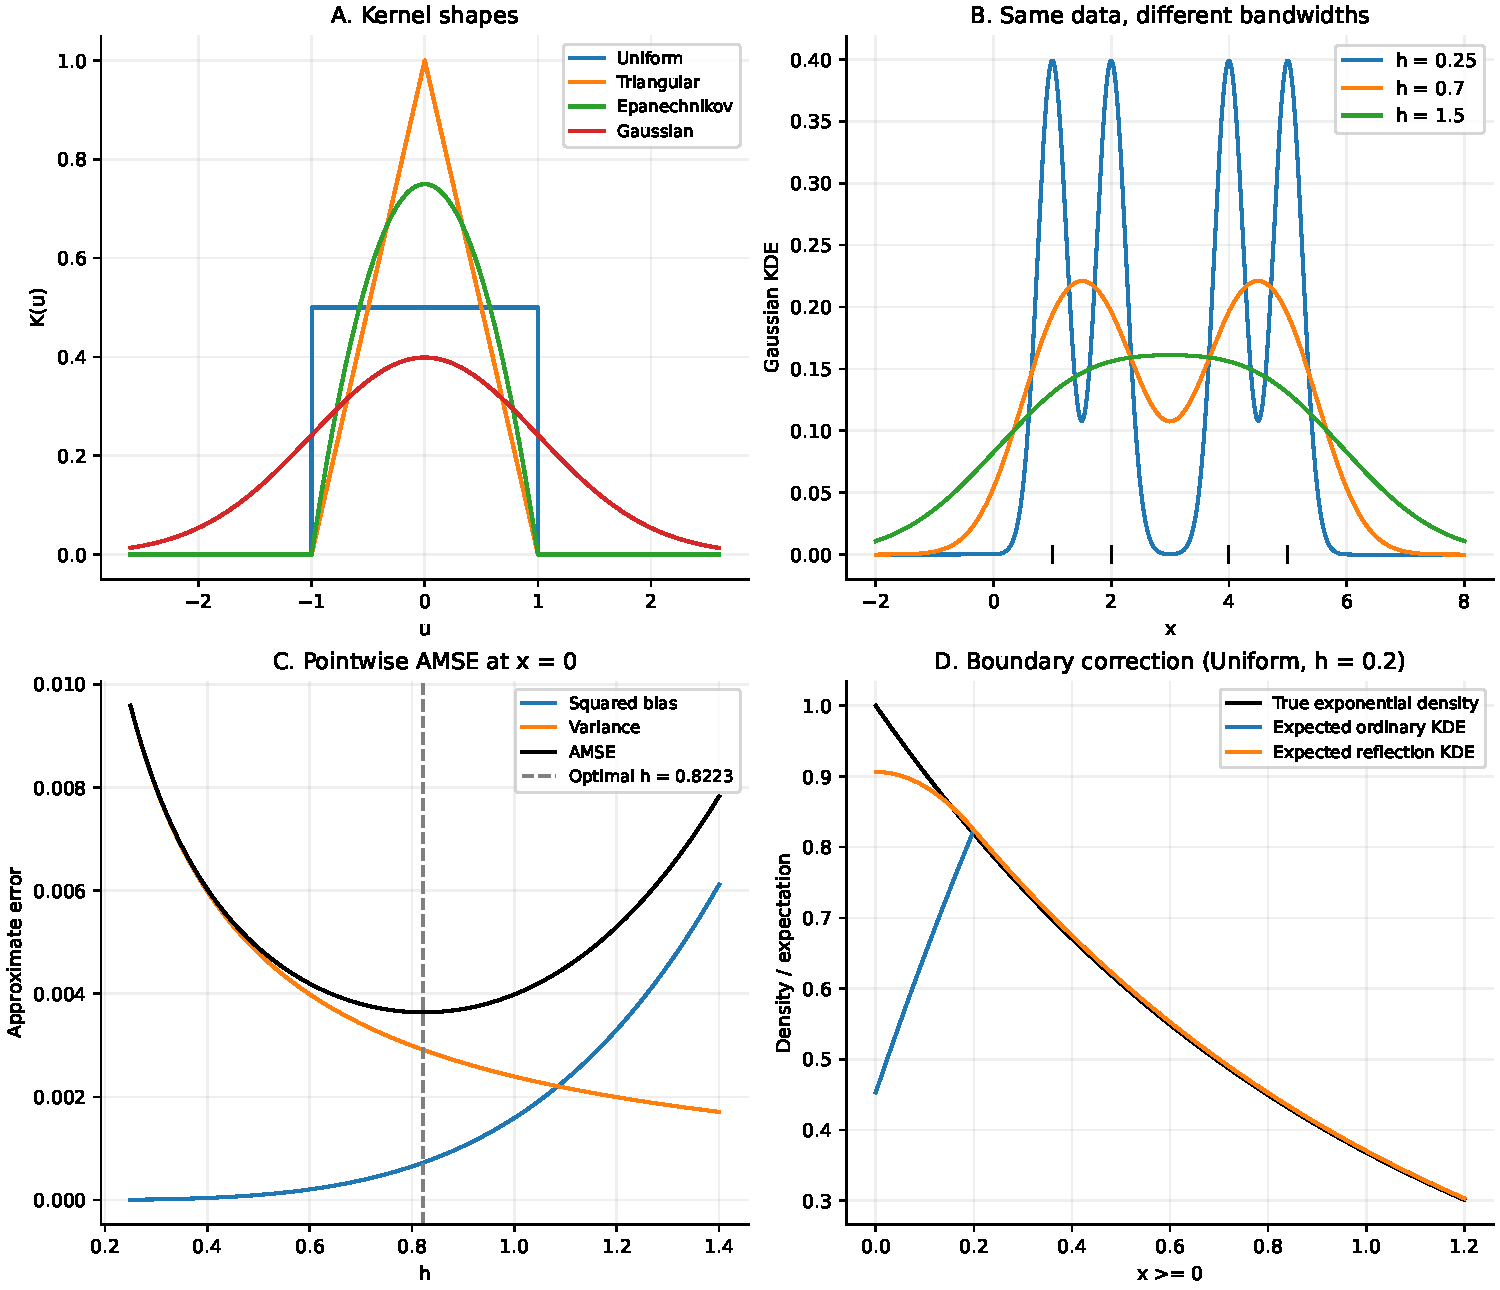
\includegraphics[width=\textwidth]{test_mo_rong_figures.pdf}
\end{center}
\textbf{Đọc hình.} Ô trên trái so sánh hình dạng các nhân theo đúng chuẩn hóa trong đề. Ô trên phải dùng cùng mẫu $(1,2,4,5)$: thay $h$ làm thay đổi số đỉnh và độ rộng của KDE Gaussian. Ô dưới trái minh họa AMSE \emph{xấp xỉ} tại 0 cho nhân Epanechnikov của đề gốc. Ô dưới phải vẽ \emph{kỳ vọng lý thuyết} của KDE Uniform ở biên cho mật độ mũ $f(x)=e^{-x}\mathbf1_{x\geq0}$, $h=0.2$, cho thấy mất khối lượng gần 0 và tác dụng của reflection; không phải một mẫu mô phỏng.

\clearpage
\section{Bảng công thức}
\subsection{Công thức liên quan}
\renewcommand{\arraystretch}{1.35}
\begin{longtable}{p{.26\textwidth}p{.67\textwidth}}
\toprule
Mục tiêu & Công thức và điều kiện cần nhớ\\
\midrule
\endhead
KDE & $\fh(x)=\frac1{nh}\sum_iK((x-X_i)/h)$; $h>0$.\\
Kỳ vọng & $\E\fh(x)=\int K(u)f(x-hu)du$.\\
Chệch bậc hai & $\Bias=\frac{h^2}2\mu_2(K)f''(x)+o(h^2)$ tại điểm nội, đủ trơn và moment.\\
Phương sai dẫn đầu & $\Var\fh(x)=\frac{R(K)f(x)}{nh}+o((nh)^{-1})$ dưới điều kiện Mục \ref{sec:variance}.\\
AMSE tại $x$ & $\frac{h^4}4\mu_2(K)^2[f''(x)]^2+\frac{R(K)f(x)}{nh}$.\\
$h_*$ tại điểm & $\left[\frac{R(K)f(x)}{n\mu_2(K)^2[f''(x)]^2}\right]^{1/5}$ nếu các hệ số dương.\\
AMISE toàn cục & $\frac{h^4}4\mu_2(K)^2R(f'')+\frac{R(K)}{nh}$.\\
$h_*$ toàn cục & $\left[\frac{R(K)}{n\mu_2(K)^2R(f'')}\right]^{1/5}$.\\
Quy tắc chuẩn & $h_{\mathrm{NR}}=(4/3)^{1/5}\widehat\sigma n^{-1/5}\approx1.06\widehat\sigma n^{-1/5}$ cho nhân Gaussian.\\
LOO & $\widehat f_{(-i),h}(X_i)=\frac1{(n-1)h}\sum_{j\ne i}K((X_i-X_j)/h)$.\\
CV bình phương & $J_{\mathrm{CV}}(h)=\int\fh^2-\frac2n\sum_i\widehat f_{(-i),h}(X_i)$.\\
Tốc độ bậc $\ell$ & $h_*\asymp n^{-1/(2\ell+1)}$, MISE $O(n^{-2\ell/(2\ell+1)})$ với đủ độ trơn $L^2$.\\
CDF làm trơn & $\widetilde F_{n,h}(x)=n^{-1}\sum_iG((x-X_i)/h)$, $G'=K$; đạo hàm là KDE.\\
Hồi quy nhân & $\widehat r(x)=\sum_i k_iY_i/\sum_i k_i$, $k_i=K((x-X_i)/h)$; mẫu số dương.\\
Histogram & $\E\widehat f=p_j/h$, $\Var\widehat f=p_j(1-p_j)/(nh^2)$ trên ô $j$.\\
CV Histogram & $\frac2{(n-1)h}-\frac{n+1}{(n-1)h}\sum_j(Y_j/n)^2$, với $n>1$.\\
Hệ số phép chiếu & $\widehat a_j=n^{-1}\sum_i\phi_j(X_i)$, $\widehat f_D=\sum_{j\leq D}\widehat a_j\phi_j$.\\
Rủi ro phép chiếu & $\|f-f_D\|_2^2+n^{-1}\sum_{j\leq D}\Var(\phi_j(X))\leq\|f-f_D\|_2^2+\phi_0D/n$.\\
Chọn mô hình & Tối thiểu hóa $-\sum_{j\leq D}\widehat a_j^2+\operatorname{pen}(D)$, với phạt hiệu chỉnh phù hợp.\\
Root--Unroot & $Y_j=\sqrt{(k/n)(N_j+1/4)}$, $\sigma^2\approx k/(4n)$; hồi quy rồi lấy phần dương, bình phương, chuẩn hóa.\\
KDE đa chiều & $\widehat f(x)=(n\prod_jh_j)^{-1}\sum_i\prod_jK((x_j-X_{ij})/h_j)$.\\
Tốc độ đa chiều & Với băng thông chung, $h_*\asymp n^{-1/(d+4)}$, AMISE $O(n^{-4/(d+4)})$ dưới độ trơn bậc hai.\\
\bottomrule
\end{longtable}

\textbf{Mẫu giải tối ưu nên thuộc.} Với $g(h)=Ah^p+B/h$, $A,B,p>0$:
\[
g'(h)=pAh^{p-1}-Bh^{-2}=0\iff h_*=(B/(pA))^{1/(p+1)},
\qquad B/h_*=pAh_*^p.
\]
Dấu của $g'$ bằng dấu của $pAh^{p+1}-B$, nên đổi từ âm sang dương duy nhất ở $h_*$. Khi đó $g(h_*)=(p+1)Ah_*^p$. Dùng $p=4$ cho KDE bậc hai, $p=2$ cho histogram, $p=2\ell$ cho nhân cấp cao.

% Included by test_loi_giai_mo_rong.tex; compile the parent with XeLaTeX.
\clearpage
% Keep the exercise subsections numbered 10.1 onward without an introductory heading.
\refstepcounter{section}\label{ot45:start}

\subsection{Phần I.A: Năm bài chứng minh cho KDE}

\subsubsection*{Bài 1.1. KDE là một mật độ xác suất hợp lệ}\label{ot45:kde-density}
\textbf{Đề bài.} Với $h>0$, $K\geq0$ và $\int_{\R}K=1$, chứng minh
$\widehat f_h(x)\geq0$ và $\int_{\R}\widehat f_h(x)dx=1$ với mọi mẫu.

\textbf{Điều kiện và công cụ.} Chỉ cần điều kiện về nhân và $h>0$;
không cần giả thiết mật độ thật trơn, cũng không cần dùng tính độc lập.

\buoc{Bước 1. Kiểm tra tính không âm.}
Mỗi số $K((x-X_i)/h)$ không âm, hệ số $1/(nh)>0$, nên tổng có trọng số không âm.

\buoc{Bước 2. Tính diện tích của một bản nhân.}
Giữ $X_i$ cố định, đặt $u=(x-X_i)/h$, $dx=h\,du$.
Khi $x$ chạy từ $-\infty$ đến $\infty$, $u$ cũng chạy trên toàn trục. Do đó
\[
\int_{\R}K\left(\frac{x-X_i}{h}\right)dx=h\int_{\R}K(u)du=h.
\]

\buoc{Bước 3. Cộng diện tích của $n$ số hạng.}
Tổng hữu hạn được đổi thứ tự với tích phân:
\[
\int_{\R}\widehat f_h(x)dx
=\frac1{nh}\sum_{i=1}^n\int_{\R}K\left(\frac{x-X_i}{h}\right)dx
=\frac{nh}{nh}=1.
\]
\textbf{Kết luận.} $\boxed{\widehat f_h\geq0,\quad\int\widehat f_h=1.}$

\textbf{Lỗi dễ mắc.} Quên $dx=h\,du$; hoặc chỉ chứng minh tích phân bằng 1 rồi kết luận là mật độ dù nhân có phần âm.

\subsubsection*{Bài 1.2. Khai triển Bias của KDE}\label{ot45:kde-bias}
\textbf{Đề bài.} Giả sử $f\in C^2(\R)$, $f''$ bị chặn,
$K\in L^1(\R)$, $\int K=1$, $\int uK(u)du=0$ và
$\int u^2|K(u)|du<\infty$. Chứng minh tại $x$ cố định:
\[
\Bias(\widehat f_h(x))=\frac{h^2}{2}\mu_2(K)f''(x)+o(h^2).
\]
Đối xứng là một điều kiện đủ để moment bậc nhất bằng 0, khi moment đó tồn tại.

\textbf{Công cụ.} Tuyến tính kỳ vọng, đổi biến, Taylor dạng phần dư tích phân và hội tụ bị chặn bởi một hàm khả tích.

\buoc{Bước 1. Viết kỳ vọng thành tích phân.}
Các quan sát cùng phân phối nên
\[
\E\widehat f_h(x)=\frac1{nh}\sum_{i=1}^n
\E K\left(\frac{x-X_i}{h}\right)
=\frac{n}{nh}\E K\left(\frac{x-X_1}{h}\right).
\]
Ở bước này chỉ cần cùng phân phối, chưa cần độc lập.
Với biến ngẫu nhiên có mật độ $f$, quy tắc $\E g(X)=\int g(t)f(t)dt$ cho
\begin{align*}
f_h(x)&=\frac1h\E K\left(\frac{x-X_1}{h}\right)
=\frac1h\int_{\R}K\left(\frac{x-t}{h}\right)f(t)dt\\
&=\int_{\R}K(u)f(x-hu)du.
\end{align*}
Ở dòng cuối, $u=(x-t)/h$, $dt=-h\,du$; dấu âm biến mất khi đảo cận.
Chi tiết: $t=x-hu$; khi $t=-\infty$ thì $u=+\infty$,
khi $t=+\infty$ thì $u=-\infty$. Vì vậy
\[
\frac1h\int_{+\infty}^{-\infty}K(u)f(x-hu)(-h)du
=\int_{-\infty}^{+\infty}K(u)f(x-hu)du.
\]

\buoc{Bước 2. Khai triển và kiểm soát phần dư.}
\textbf{Ý tưởng.} Với $u$ cố định và $h$ nhỏ, $x-hu$ gần $x$.
Taylor diễn tả giá trị tại điểm gần đó bằng giá trị, độ dốc và độ cong tại $x$.
Công thức quen thuộc là
$f(x+v)=f(x)+vf'(x)+v^2f''(x)/2+\text{phần dư}$.
Thay $v=-hu$; khi đó $v^2=h^2u^2$, nên dấu của hạng bậc hai là dấu cộng:
\[
f(x-hu)=f(x)-hu f'(x)+\frac{h^2u^2}{2}f''(x)+r_h(u),
\]
với
\[
r_h(u)=h^2u^2\int_0^1(1-s)\{f''(x-shu)-f''(x)\}ds.
\]
\textbf{Phần dư tích phân đến từ đâu?}
Với một độ dịch cố định $v$, đặt $F(s)=f(x+sv)$ trên $0\leq s\leq1$.
Quy tắc hàm hợp cho $F'(s)=vf'(x+sv)$, $F''(s)=v^2f''(x+sv)$.
Tích phân từng phần cho
\[
\int_0^1(1-s)F''(s)ds
=[(1-s)F'(s)]_0^1+\int_0^1F'(s)ds
=-F'(0)+F(1)-F(0).
\]
Chuyển vế, rồi thay lại $F$, được công thức chính xác
\[
f(x+v)=f(x)+vf'(x)+v^2\int_0^1(1-s)f''(x+sv)ds.
\]
Tách $f''(x+sv)$ thành $f''(x)+[f''(x+sv)-f''(x)]$;
phần thứ nhất có tích phân $f''(x)/2$.
Phần thứ hai chính là phần dư ở trên khi thay $v=-hu$.

\textbf{Vì sao phần dư nhỏ sau khi tích phân theo nhân?}
Với từng $u$ cố định, $r_h(u)/h^2\to0$ do $f''$ liên tục tại $x$.
Nếu $M=\|f''\|_\infty$, thì
$|r_h(u)|/h^2\leq Mu^2$.
Thật vậy, hiệu hai giá trị $f''$ có trị tuyệt đối không quá $2M$ và
$\int_0^1(1-s)ds=1/2$, nên chặn là $u^2\cdot2M\cdot(1/2)=Mu^2$.
Vì $Mu^2|K(u)|$ khả tích, định lý hội tụ bị chặn cho
\[
\frac1{h^2}\int K(u)r_h(u)du\longrightarrow0.
\]
Đây là lý do được đưa phần dư qua dấu tích phân.

\buoc{Bước 3. Dùng các moment của nhân.}
Nhân từng hạng Taylor với $K(u)$ rồi tích phân theo $u$.
Các hệ số $f(x),hf'(x),h^2f''(x)/2$ không phụ thuộc $u$:
\begin{align*}
f_h(x)&=f(x)\int K-hf'(x)\int uK
+\frac{h^2}{2}f''(x)\int u^2K+o(h^2)\\
&=f(x)+\frac{h^2}{2}\mu_2(K)f''(x)+o(h^2).
\end{align*}
Ba phép thay ở dòng cuối lần lượt là
$\int K=1$, $\int uK=0$, $\int u^2K=\mu_2(K)$.
Hạng chứa $f'(x)$ biến mất do moment bậc nhất bằng 0, không phải vì $f'(x)=0$.
\textbf{Kết luận.} Trừ $f(x)$ thu được công thức đề bài.
Nếu $f''(x)=0$, hệ số dẫn đầu triệt tiêu và Bias chỉ còn $o(h^2)$.

\textbf{Lỗi dễ mắc.} Viết $O(h^4)$ chỉ từ giả thiết $C^2$;
hoặc dùng khai triển tại một điểm rồi tích phân phần dư mà không có điều kiện kiểm soát.

\subsubsection*{Bài 1.3. Phương sai chính xác và tiệm cận}\label{ot45:kde-variance}
\textbf{Đề bài.} Giả sử $f$ bị chặn và liên tục tại $x$,
$K\in L^1\cap L^2$, $\int K=1$. Chứng minh
\[
\Var(\widehat f_h(x))
=\frac1{nh}\int K(u)^2f(x-hu)du-\frac{f_h(x)^2}{n}
=\frac{f(x)R(K)}{nh}+o((nh)^{-1}).
\]

\textbf{Công cụ.} Các quan sát độc lập; $\Var Z=\E Z^2-(\E Z)^2$;
đổi biến và hội tụ bị chặn.

\buoc{Bước 1. Rút về phương sai của một quan sát.}
Đặt $Z_i=K((x-X_i)/h)$. Do độc lập,
ta dùng $\Var(cY)=c^2\Var(Y)$ và
$\Var(\sum_iZ_i)=\sum_i\Var(Z_i)$.
Các $Z_i$ cùng phân phối nên tổng cuối có $n$ số hạng bằng nhau:
\[
\Var(\widehat f_h(x))=\frac{1}{n^2h^2}\sum_i\Var Z_i
=\frac{1}{nh^2}\{\E Z_1^2-(\E Z_1)^2\}.
\]

\buoc{Bước 2. Tính hai moment bằng đổi biến.}
Đối với moment bậc hai, bình phương $Z_1$ trước khi lấy kỳ vọng:
\begin{align*}
\E Z_1^2
&=\int_{-\infty}^{+\infty}K\left(\frac{x-t}{h}\right)^2f(t)dt\\
&=\int_{+\infty}^{-\infty}K(u)^2f(x-hu)(-h)du
=h\int_{\R}K(u)^2f(x-hu)du.
\end{align*}
Đổi biến tương tự cho moment bậc nhất:
\[
\E Z_1^2=h\int K(u)^2f(x-hu)du,\qquad \E Z_1=hf_h(x).
\]
Thế vào Bước 1 và chia từng số hạng:
\begin{align*}
\Var(\widehat f_h(x))
&=\frac1{nh^2}\left[h\int K(u)^2f(x-hu)du-h^2f_h(x)^2\right]\\
&=\frac1{nh}\int K(u)^2f(x-hu)du-\frac{f_h(x)^2}{n}.
\end{align*}
Lưu ý $\E Z_1^2$ và $(\E Z_1)^2$ là hai đại lượng khác nhau.

\buoc{Bước 3. Xác định số hạng chính và phần dư.}
\textbf{Ý tưởng.} Khi $h\to0$, với mỗi $u$ cố định ta có
$f(x-hu)\to f(x)$. Ta muốn thay mật độ trong tích phân bằng $f(x)$.
Chặn khả tích dưới đây cho phép đưa giới hạn qua dấu tích phân.
Vì $|K(u)^2f(x-hu)|\leq\|f\|_\infty K(u)^2$ khả tích,
\[
\int K(u)^2f(x-hu)du=f(x)R(K)+o(1).
\]
Mặt khác $|f_h(x)|\leq\|f\|_\infty\|K\|_1$, nên
\[
\frac{f_h(x)^2}{n}=O(1/n)=o((nh)^{-1}),
\qquad\frac{1/n}{1/(nh)}=h\to0.
\]
\textbf{Kết luận.} $\boxed{\Var(\widehat f_h(x))=f(x)R(K)/(nh)+o((nh)^{-1}).}$
Nếu $f(x)=0$, kết luận là $o((nh)^{-1})$, không phải tương đương với một số dương.

\textbf{Lỗi dễ mắc.} Bỏ bình phương của $1/h$ khi lấy phương sai;
hoặc bỏ $-(\E Z_1)^2$ mà chưa giải thích bậc của nó.

\subsubsection*{Bài 1.4. Tối ưu AMSE, AMISE và tốc độ}\label{ot45:kde-optimal}
\textbf{Đề bài.} Cho $X_1,\ldots,X_n$ độc lập cùng mật độ $f$ trên $\R$ và
\[
\widehat f_h(x)=\frac1{nh}\sum_{i=1}^nK\left(\frac{x-X_i}{h}\right),\qquad
f_h=\E\widehat f_h,\quad R(g)=\int_{\R}g^2.
\]
Giả sử $K\in L^1\cap L^2$, $\int K=1$, $\int uK(u)du=0$,
$\int u^2|K(u)|du<\infty$ và $\mu_2(K)=\int u^2K(u)du\ne0$.
Mật độ $f$ bị chặn, thuộc $C^2(\R)\cap W^{2,2}(\R)$, $f''$ bị chặn;
$h=h_n\to0$, $nh_n\to\infty$. Tại điểm xét, $f(x)>0$, $f''(x)\ne0$.
\begin{enumerate}[label=(\alph*)]
\item Từ các số hạng dẫn đầu
$\Bias(\widehat f_h(x))=h^2\mu_2(K)f''(x)/2+o(h^2)$ và
$\Var(\widehat f_h(x))=f(x)R(K)/(nh)+o((nh)^{-1})$,
lập và tối ưu AMSE tại $x$.
\item Chứng minh phân rã MISE chính xác; kiểm soát phần dư theo $L^2$ để suy ra
$\AMISE(h)=h^4\mu_2(K)^2R(f'')/4+R(K)/(nh)$.
Giải thích vì sao AMISE không phải MISE chính xác.
\item Với $R(f'')>0$, tìm $h_{\mathrm{AMISE},*}$, chứng minh cực tiểu toàn cục,
tính hằng số của AMISE nhỏ nhất và tốc độ theo $n$.
\end{enumerate}

\textbf{Công cụ.} Phân rã MSE thành bình phương Bias cộng phương sai;
đạo hàm hàm $Ah^4+B/(nh)$ với $A,B>0$.
$W^{2,2}$ nghĩa là $f$ và các đạo hàm yếu đến bậc hai thuộc $L^2$.
\textbf{Lời giải ý (a).}

\buoc{Bước 1. Tối ưu sai số tại một điểm.}
\textbf{Từ Bias sang AMSE:} bình phương hạng Bias chính cho
$[h^2\mu_2(K)f''(x)/2]^2=h^4\mu_2(K)^2[f''(x)]^2/4$,
rồi cộng hạng phương sai chính. Ta tìm $h>0$ làm tổng này nhỏ nhất.
Đặt $A_x=\mu_2(K)^2[f''(x)]^2/4$, $B_x=f(x)R(K)$. Khi đó
\[
\AMSE_x(h)=A_xh^4+\frac{B_x}{nh},\quad
\AMSE_x'(h)=4A_xh^3-\frac{B_x}{nh^2}.
\]
Để thấy rõ đạo hàm, viết $B_x/(nh)=(B_x/n)h^{-1}$.
Khi đó $(A_xh^4)'=4A_xh^3$ và $[(B_x/n)h^{-1}]'=-(B_x/n)h^{-2}$.
Giải phương trình bằng cách nhân hai vế với $h^2>0$:
\[
4A_xh^3=\frac{B_x}{nh^2}
\ \Longleftrightarrow\ 4A_xh^5=\frac{B_x}{n}
\ \Longleftrightarrow\ h^5=\frac{B_x}{4A_xn}.
\]
Lấy căn bậc năm dương và thay $4A_x=\mu_2(K)^2[f''(x)]^2$, được
\[
\boxed{h_{x,*}=\left[\frac{f(x)R(K)}{n\mu_2(K)^2[f''(x)]^2}\right]^{1/5}.}
\]
Đạo hàm bậc hai $12A_xh^2+2B_x/(nh^3)>0$; hàm tiến ra vô cực khi $h\downarrow0$
hoặc $h\to\infty$, nên đây là cực tiểu toàn cục của AMSE.
Đạo hàm bậc hai dương nghĩa là đạo hàm bậc nhất tăng nghiêm ngặt;
trước nghiệm hàm giảm, sau nghiệm hàm tăng. Vì vậy nghiệm là điểm nhỏ nhất duy nhất.

\buoc{Bước 2. Thế nghiệm để xác định tốc độ và hằng số.}
Tại nghiệm, $B_x/(nh_{x,*})=4A_xh_{x,*}^4$. Vì vậy
hai số hạng của AMSE cộng thành $A_xh_{x,*}^4+4A_xh_{x,*}^4=5A_xh_{x,*}^4$.
Để rút gọn, dùng $(ab)^p=a^pb^p$ và $a^pa^q=a^{p+q}$ với các cơ số dương:
\[
5A_x\left(\frac{B_x}{4A_xn}\right)^{4/5}
=5\,4^{-4/5}A_x^{1/5}B_x^{4/5}n^{-4/5}.
\]
Thay $A_x=\mu_2(K)^2[f''(x)]^2/4$ làm hệ số chứa 4 thành
$4^{-4/5}4^{-1/5}=1/4$, nên
\[
\AMSE_x(h_{x,*})=5A_xh_{x,*}^4
=\frac54\{\mu_2(K)^2[f''(x)]^2\}^{1/5}
\{f(x)R(K)\}^{4/5}n^{-4/5}.
\]
Hai số hạng không bằng nhau: phương sai xấp xỉ bằng bốn lần bình phương Bias.

\textbf{Lời giải ý (b).}
\buoc{Bước 3. Phân rã MISE chính xác trước khi dùng xấp xỉ.}
Tại mỗi $x$, viết
$\widehat f_h-f=(\widehat f_h-f_h)+(f_h-f)$.
Hạng chéo có kỳ vọng 0 vì $\E(\widehat f_h-f_h)=0$.
Để thấy rõ, viết $U=\widehat f_h(x)-f_h(x)$ và $b=f_h(x)-f(x)$,
trong đó $b$ không ngẫu nhiên:
\[
\E(U+b)^2=\E U^2+2b\E U+b^2=\Var(\widehat f_h(x))+b^2.
\]
Suy ra
\[
\E(\widehat f_h(x)-f(x))^2
=\Var(\widehat f_h(x))+(f_h(x)-f(x))^2.
\]
Tonelli cho phép đổi kỳ vọng và tích phân của bình phương không âm:
\[
\boxed{\MISE(h)=\E\|\widehat f_h-f\|_2^2
=\int_{\R}\MSE_x(h)dx
=\|f_h-f\|_2^2+\int_{\R}\Var(\widehat f_h(x))dx.}
\]

\buoc{Bước 4. Kiểm soát bình phương chệch trên toàn trục.}
\textbf{Ý tưởng.} Cần xấp xỉ tốt cho toàn bộ hàm, đo bằng chuẩn $L^2$,
để sau đó bình phương và tích phân. Ký hiệu $f''(\,\cdot-a)$ nghĩa là
hàm $x\mapsto f''(x-a)$, tức đường $f''$ được dịch đi một đoạn $a$.
Taylor dạng tích phân và hai moment đầu của $K$ cho
\[
f_h-f=h^2\int u^2K(u)\int_0^1(1-t)f''(\,\cdot-thu)dt\,du.
\]
Trừ $h^2\mu_2(K)f''/2$, chia cho $h^2$ và lấy chuẩn $L^2$:
\begin{align*}
\left\|\frac{f_h-f}{h^2}-\frac{\mu_2(K)}2f''\right\|_2
&\leq\int |u|^2|K(u)|\int_0^1(1-t)
\|f''(\,\cdot-thu)-f''\|_2dt\,du\\
&\longrightarrow0.
\end{align*}
Giới hạn dùng tính liên tục của phép tịnh tiến trong $L^2$;
chuẩn trong tích phân không vượt $2\|f''\|_2$, còn $u^2|K(u)|$ khả tích.
Vì vậy có phần dư $r_h$ với $\|r_h\|_2=o(h^2)$ sao cho
$f_h-f=h^2\mu_2(K)f''/2+r_h$. Khai triển bình phương chuẩn và dùng
Cauchy--Schwarz cho hạng chéo như sau.
Đặt $g=\mu_2(K)f''/2$, khi đó
\[
\|h^2g+r_h\|_2^2=h^4\|g\|_2^2+2h^2\langle g,r_h\rangle+\|r_h\|_2^2.
\]
Vì $|\langle g,r_h\rangle|\leq\|g\|_2\|r_h\|_2$,
hạng chéo có trị tuyệt đối không quá $2h^2\|g\|_2o(h^2)=o(h^4)$;
hạng cuối cũng là $o(h^4)$. Do đó
\[
\|f_h-f\|_2^2=\frac{h^4}{4}\mu_2(K)^2R(f'')+o(h^4).
\]
Đây là điều kiện tích phân thực sự cần; chỉ có khai triển tại từng điểm chưa đủ.

\buoc{Bước 5. Tính phương sai tích phân và nhận diện AMISE.}
Độc lập của mẫu và đổi biến cho công thức chính xác
\[
\Var(\widehat f_h(x))
=\frac1{nh}\int K(u)^2f(x-hu)du-\frac{f_h(x)^2}{n}.
\]
Tích phân hạng đầu dùng Tonelli và $\int f(x-hu)dx=1$, nên
\[
\frac1{nh}\int_{\R}\int_{\R}K(u)^2f(x-hu)du\,dx
=\frac1{nh}\int_{\R}K(u)^2
\underbrace{\left[\int_{\R}f(x-hu)dx\right]}_{=1}du
=\frac{R(K)}{nh}.
\]
Ở tích phân trong, $t=x-hu$ có $dt=dx$ vì $u$ đang được giữ cố định.
Vì vậy
\[
\int\Var(\widehat f_h(x))dx=\frac{R(K)}{nh}-\frac{R(f_h)}n.
\]
Do $\|f_h\|_2\leq\|K\|_1\|f\|_2$, hạng cuối là $O(1/n)$.
Vì $h\to0$, $1/n=o((nh)^{-1})$. Kết hợp các bước trên:
\[
\MISE(h)=\frac{h^4}{4}\mu_2(K)^2R(f'')+\frac{R(K)}{nh}
+o\left(h^4+\frac1{nh}\right).
\]
Ta gọi tổng hai số hạng chính là
\[
\AMISE(h)=\frac{h^4}{4}\mu_2(K)^2R(f'')+\frac{R(K)}{nh}.
\]
Đẳng thức $\int\MSE_x(h)dx=\MISE(h)$ là chính xác;
thay MSE bằng các số hạng tiệm cận chính mới cho AMISE.

\textbf{Lời giải ý (c).}
\buoc{Bước 6. Đạo hàm và kiểm tra cực tiểu toàn cục.}
Đặt $A=\mu_2(K)^2R(f'')/4>0$, $B=R(K)>0$.
Đây chính là bài toán $Ah^4+(B/n)h^{-1}$ đã giải ở ý (a),
với $[f''(x)]^2$ được thay bằng tích phân $R(f'')$.
\[
\AMISE'(h)=4Ah^3-\frac{B}{nh^2}=0
\quad\Longleftrightarrow\quad h^5=\frac{B}{4An}.
\]
Vì $\AMISE''(h)=12Ah^2+2B/(nh^3)>0$ trên $h>0$ và AMISE
tiến ra vô cực tại cả hai đầu miền, nghiệm là cực tiểu toàn cục duy nhất:
\[
\boxed{h_{\mathrm{AMISE},*}
=\left[\frac{R(K)}{n\mu_2(K)^2R(f'')}\right]^{1/5},}
\]
\buoc{Bước 7. Thế nghiệm để tìm hằng số và tốc độ.}
Tại nghiệm, $B/(nh_*)=4Ah_*^4$, nên
\[
Ah_*^4+\frac{B}{nh_*}=5Ah_*^4
=5A\left(\frac{B}{4An}\right)^{4/5}
=5\,4^{-4/5}A^{1/5}B^{4/5}n^{-4/5}.
\]
Thay lại $A,B$ như ở ý (a) cho
\[
\AMISE(h_{\mathrm{AMISE},*})
=\frac54\{\mu_2(K)^2R(f'')\}^{1/5}R(K)^{4/5}n^{-4/5}.
\]
\textbf{Kết luận.} Cả hai bandwidth đều có bậc $n^{-1/5}$;
AMSE/AMISE tối ưu có bậc $n^{-4/5}$. Với khai triển MISE ở trên,
MISE tại bandwidth AMISE cũng đạt $O(n^{-4/5})$.
Bandwidth tối ưu AMISE không được khẳng định là nghiệm chính xác của MISE hữu hạn mẫu.

\textbf{Lỗi dễ mắc.} Dùng $f''(x)^2$ thay $R(f'')$ khi tối ưu toàn trục;
áp dụng công thức điểm khi $f''(x)=0$; hoặc viết tốc độ bandwidth thành tốc độ rủi ro.

\subsubsection*{Bài 1.5. Nhân cấp cao và tốc độ tổng quát}\label{ot45:highorder}
\textbf{Đề bài.} Cho số nguyên $\ell>2$, $K\in L^1\cap L^2$ thỏa
\[
\int K=1,\quad\mu_j(K)=0\ (1\leq j<\ell),\quad
\mu_\ell(K)\ne0,\quad M_\ell:=\int |u|^\ell|K(u)|du<\infty.
\]
Chứng minh Bias bậc $h^\ell$, rồi tìm bậc bandwidth và MISE.
Phần tại điểm dùng $f\in C^\ell$ với $f^{(\ell)}$ bị chặn;
phần MISE dùng $f\in W^{\ell,2}(\R)$.

\textbf{Công cụ.} Taylor, moment triệt tiêu, bất đẳng thức tam giác tích phân trong $L^2$ và tối ưu hàm hai số hạng.

\buoc{Bước 1. Tính Bias tại một điểm.}
\textbf{Đọc trường hợp bậc 4 trước.} Nếu $\ell=4$, Taylor có các hạng
\[
f(x-hu)=f(x)-hu f'(x)+\frac{h^2u^2}{2}f''(x)
-\frac{h^3u^3}{6}f^{(3)}(x)+\frac{h^4u^4}{24}f^{(4)}(x)+r_h(u).
\]
Sau khi nhân với $K$ và tích phân, ba hạng bậc $1,2,3$ mất đi vì
$\mu_1=\mu_2=\mu_3=0$. Trừ $f(x)$, chỉ còn hạng bậc 4 và phần dư.
Đối với bậc tổng quát, cách làm vẫn như vậy; $j!=1\cdot2\cdots j$
và $f^{(j)}$ là đạo hàm lần thứ $j$.
Với $x$ cố định, Taylor đến bậc $\ell$ cho
\[
f(x-hu)=\sum_{j=0}^{\ell}\frac{(-hu)^j}{j!}f^{(j)}(x)+r_h(u).
\]
Ở bậc tổng quát, phần dư có biểu thức
\[
r_h(u)=\frac{(-hu)^\ell}{(\ell-1)!}
\int_0^1(1-t)^{\ell-1}
\{f^{(\ell)}(x-thu)-f^{(\ell)}(x)\}dt.
\]
Nếu $M=\|f^{(\ell)}\|_\infty$, trị tuyệt đối của hiệu trong ngoặc không quá $2M$,
và $\int_0^1(1-t)^{\ell-1}dt=1/\ell$. Do đó
$|r_h(u)|/h^\ell\leq 2M|u|^\ell/\ell!$.
Với mỗi $u$ cố định, tỉ số phần dư tiến về 0 do tính liên tục của $f^{(\ell)}$.
Nhân chặn với $|K(u)|$ cho một hàm khả tích nhờ $M_\ell<\infty$;
hội tụ bị chặn cho $\int K(u)r_h(u)du=o(h^\ell)$ như Bài 1.2.
Vì các moment từ 1 đến $\ell-1$ bằng 0,
ta có thể viết rõ từng hệ số sau tích phân:
\[
f_h(x)-f(x)=\sum_{j=1}^{\ell}
\frac{(-h)^j}{j!}f^{(j)}(x)\underbrace{\int u^jK(u)du}_{\mu_j(K)}
+o(h^\ell).
\]
Trong tổng, chỉ số $j=\ell$ có thể còn lại. Do đó
\[
\boxed{\Bias(\widehat f_h(x))
=\frac{(-1)^\ell\mu_\ell(K)}{\ell!}h^\ell f^{(\ell)}(x)+o(h^\ell)=O(h^\ell).}
\]

\buoc{Bước 2. Chứng minh một chặn tích phân, thay vì chỉ dùng Bias tại điểm.}
\textbf{Ý tưởng.} Chặn độ lớn của toàn bộ hàm Bias trước, rồi bình phương
để chặn sai số tích phân. Khi dịch biến, tích phân trên toàn trục không đổi:
$\int|f^{(\ell)}(x-a)|^2dx=\int|f^{(\ell)}(y)|^2dy$ với $y=x-a$.
Taylor dạng tích phân, sau khi tích phân theo $K$ và triệt tiêu các moment, cho
\[
f_h-f=\frac{(-h)^\ell}{(\ell-1)!}
\int_{\R}u^\ell K(u)\int_0^1(1-t)^{\ell-1}
f^{(\ell)}(\,\cdot-thu)dt\,du.
\]
Phép tịnh tiến không đổi chuẩn $L^2$. Lấy chuẩn, dùng bất đẳng thức tam giác
và $\int_0^1(1-t)^{\ell-1}dt=1/\ell$, được
\[
\|f_h-f\|_2\leq\frac{M_\ell}{\ell!}\|f^{(\ell)}\|_2h^\ell=:C_\ell h^\ell.
\]
Hệ số giai thừa đến từ
$1/[(\ell-1)!]\cdot1/\ell=1/\ell!$.
Bình phương hai vế cho $\|f_h-f\|_2^2\leq C_\ell^2h^{2\ell}$.
Đây là bước bổ sung cần thiết để suy ra MISE trên toàn trục.
Kết hợp phương sai tích phân chính xác, có
\[
\MISE(h)\leq C_\ell^2h^{2\ell}+\frac{R(K)}{nh}.
\]

\buoc{Bước 3. Tối ưu chặn trên.}
Với $C_\ell>0$, đạo hàm vế phải bằng 0 khi
\[
2\ell C_\ell^2h^{2\ell-1}-\frac{R(K)}{nh^2}=0,
\qquad h_*=
\left[\frac{R(K)}{2\ell C_\ell^2 n}\right]^{1/(2\ell+1)}.
\]
Chi tiết giải phương trình: chuyển hạng âm sang vế phải và nhân với $h^2$:
\[
2\ell C_\ell^2h^{2\ell+1}=\frac{R(K)}n,
\qquad h^{2\ell+1}=\frac{R(K)}{2\ell C_\ell^2n}.
\]
Hàm chặn có đạo hàm bậc hai
$2\ell(2\ell-1)C_\ell^2h^{2\ell-2}+2R(K)/(nh^3)>0$,
nên nghiệm dương trên là cực tiểu duy nhất.
Viết $h_*=c\,n^{-1/(2\ell+1)}$ với $c>0$ không phụ thuộc $n$.
Khi đó $h_*^{2\ell}=c^{2\ell}n^{-2\ell/(2\ell+1)}$ và
\[
\frac1{nh_*}=c^{-1}n^{-1+1/(2\ell+1)}
=c^{-1}n^{-2\ell/(2\ell+1)}.
\]
Thế nghiệm vào cả hai hạng:
\[
h_*^{2\ell}\asymp n^{-2\ell/(2\ell+1)},\quad
\frac1{nh_*}\asymp n^{-2\ell/(2\ell+1)}.
\]
\textbf{Kết luận.} $\boxed{h_*\asymp n^{-1/(2\ell+1)},\quad
\MISE(h_*)=O(n^{-2\ell/(2\ell+1)}).}$
Đây là tối ưu của chặn trên vừa chứng minh.
Tính liên tục của phép tịnh tiến trong $L^2$ còn cho khai triển AMISE với
$A_\ell=\mu_\ell(K)^2R(f^{(\ell)})/(\ell!)^2$ thay $C_\ell^2$,
và cùng tốc độ.

\textbf{Ví dụ cụ thể.} Với $\varphi$ là mật độ chuẩn tắc,
$K_4(u)=(3-u^2)\varphi(u)/2$ có
$\mu_1=\mu_2=\mu_3=0$, $\mu_4=(3\cdot3-15)/2=-3$.
Do đó Bias $=-h^4f^{(4)}(x)/8+o(h^4)$ và tốc độ MISE là $n^{-8/9}$.
Các moment chuẩn $\E Z^2=1$, $\E Z^4=3$, $\E Z^6=15$ cho những phép tính này.
Để kiểm tra từng moment: $\int K_4=(3-1)/2=1$;
$\mu_2(K_4)=(3\E Z^2-\E Z^4)/2=(3-3)/2=0$.
Hai moment lẻ bằng 0 do hàm dưới dấu tích phân là hàm lẻ.
Hệ số Bias bậc 4 là $\mu_4/4!=-3/24=-1/8$;
số mũ rủi ro là $2\ell/(2\ell+1)=8/9$ khi $\ell=4$.

\textbf{Lỗi dễ mắc.} Với $\ell>2$, điều kiện $\mu_2=0$ buộc nhân phải có phần âm:
nếu $K\geq0$, $\int u^2K=0$ buộc $K=0$ hầu khắp nơi ngoài $u=0$, trái $\int K=1$.
Vì thế KDE cấp cao không tự động là mật độ không âm.
Nhân đối xứng không thể có moment đầu tiên khác 0 ở bậc lẻ.

\subsection{Phần I.B: Năm bài chứng minh cho ước lượng chiếu}
Trong nhóm này, miền là $[0,1]$, $f\in L^2([0,1])$.
$\phi_1,\ldots,\phi_D$ là các hàm thực trực chuẩn theo tích phân Lebesgue,
$S_D=\operatorname{span}(\phi_1,\ldots,\phi_D)$ và
\[
a_j=\int_0^1f\phi_j,\quad \widehat a_j=\frac1n\sum_i\phi_j(X_i),\quad
f_D=\sum_{j=1}^Da_j\phi_j,\quad \widehat f_D=\sum_{j=1}^D\widehat a_j\phi_j.
\]
Giả sử $\E\phi_j(X)^2<\infty$ khi tính phương sai.
Hai bài 2.2--2.3 phát biểu trên $\R$; bài có miền $[0,1]$ được xem là trường hợp riêng
bằng cách mở rộng các hàm bằng 0 ngoài miền.

\subsubsection*{Bài 2.1. Hệ số mẫu là ước lượng không chệch}\label{ot45:projection-coeff}
\textbf{Đề bài.} Chứng minh $\E\widehat a_j=a_j$, tính phương sai
và giải thích vì sao $\widehat f_D$ vẫn có thể chệch so với $f$.

\textbf{Công cụ.} Kỳ vọng của hàm theo mật độ, tuyến tính kỳ vọng,
phương sai trung bình các quan sát độc lập.

\buoc{Bước 1. Nhận diện hệ số thật là một kỳ vọng.}
\[
\E\phi_j(X_1)=\int_0^1\phi_j(x)f(x)dx=a_j.
\]
Tích phân tuyệt đối hữu hạn do Cauchy--Schwarz:
$\int|\phi_j f|\leq\|\phi_j\|_2\|f\|_2=\|f\|_2$.

\buoc{Bước 2. Lấy kỳ vọng và phương sai của trung bình.}
Đặt $Y_i=\phi_j(X_i)$ với $j$ cố định.
Khi đó $\widehat a_j=(Y_1+\cdots+Y_n)/n$.
Các $Y_i$ độc lập cùng phân phối, nên
\[
\Var(\widehat a_j)=\frac1{n^2}\sum_{i=1}^n\Var(Y_i)
=\frac1n\Var(Y_1)
=\frac1n\{\E Y_1^2-(\E Y_1)^2\}.
\]
Ở đây $\E Y_1=a_j$ và $\E Y_1^2=\int_0^1\phi_j(x)^2f(x)dx$.
Tương tự, tính tuyến tính cho $\E\widehat a_j=(1/n)\sum_i\E Y_i$. Vì vậy
\[
\E\widehat a_j=\frac1n\sum_i a_j=a_j,\qquad
\Var(\widehat a_j)=\frac1n\left(\int_0^1\phi_j(x)^2f(x)dx-a_j^2\right).
\]

\buoc{Bước 3. Phân biệt hai đối tượng được ước lượng.}
\[
\E\widehat f_D(x)=\sum_{j=1}^Da_j\phi_j(x)=f_D(x).
\]
\textbf{Kết luận.} Hệ số mẫu không chệch cho $a_j$;
$\widehat f_D$ không chệch cho $f_D$, nhưng có chệch $f_D-f$ so với mật độ thật.

\textbf{Lỗi dễ mắc.} Suy từ hệ số không chệch thành $\E\widehat f_D=f$ dù đã cắt chuỗi.

\subsubsection*{Bài 2.2. Tối thiểu hóa hàm tương phản}\label{ot45:contrast}
\textbf{Đề bài.} Cho mẫu độc lập $X_1,\ldots,X_n$ cùng mật độ $f\in L^2(\R)$,
không gian $S_D\subset L^2(\R)$ có cơ sở thực trực chuẩn $\phi_1,\ldots,\phi_D$.
Giả sử $\E\phi_j(X)^2<\infty$. Đặt
\[
a_j=\int_{\R}f\phi_j,\quad \widehat a_j=\frac1n\sum_i\phi_j(X_i),\quad
f_D=\sum_ja_j\phi_j,\quad \widehat f_D=\sum_j\widehat a_j\phi_j,
\]
\[
\gamma_n(g)=\|g\|_2^2-\frac2n\sum_i g(X_i),\qquad
V_D=\E\|\widehat f_D-f_D\|_2^2.
\]
\begin{enumerate}[label=(\alph*)]
\item Chứng minh nghiệm duy nhất của $\min_{g\in S_D}\gamma_n(g)$ là $\widehat f_D$
và tìm giá trị tương phản tại nghiệm. Không áp đặt thêm $g\geq0$.
\item Chứng minh $\E\|\widehat f_D\|_2^2=\|f_D\|_2^2+V_D$.
Vì sao chỉ thay $-\|f_D\|_2^2$ bằng $-\|\widehat f_D\|_2^2$ làm xuất hiện một độ lạc quan $V_D$?
\end{enumerate}

\textbf{Công cụ.} Trực chuẩn và hoàn thành bình phương.
Viết $g$ thay vì $h$ để tránh nhầm hàm ứng viên với bandwidth.
\textbf{Lời giải ý (a).}

\buoc{Bước 1. Viết tương phản theo các hệ số.}
\textbf{Vì sao trực chuẩn giúp tính toán?} Trực chuẩn nghĩa là
$\int\phi_j\phi_k=0$ khi $j\ne k$ và bằng 1 khi $j=k$.
Khai triển bình phương tổng trước khi tích phân:
\[
\left\|\sum_jb_j\phi_j\right\|_2^2
=\sum_j\sum_k b_jb_k\int\phi_j(x)\phi_k(x)dx
=\sum_jb_j^2.
\]
Các tích chéo $j\ne k$ mất đi nhờ tích phân, không cần các hệ số độc lập.
Với $g=\sum_{j=1}^D b_j\phi_j$, trực chuẩn cho $\|g\|_2^2=\sum_jb_j^2$;
đồng thời
\[
\frac1n\sum_i g(X_i)=\sum_j b_j\left(\frac1n\sum_i\phi_j(X_i)\right)
=\sum_jb_j\widehat a_j.
\]

\buoc{Bước 2. Hoàn thành bình phương.}
Với hai số $b,a$, ta có $(b-a)^2=b^2-2ba+a^2$,
nên $b^2-2ba=(b-a)^2-a^2$. Áp dụng riêng cho từng $j$:
\[
\gamma_n(g)=\sum_{j=1}^D(b_j^2-2b_j\widehat a_j)
=\sum_{j=1}^D(b_j-\widehat a_j)^2-\sum_{j=1}^D\widehat a_j^2.
\]
Hạng cuối không phụ thuộc $b_j$; tổng bình phương nhỏ nhất bằng 0,
đạt được duy nhất khi mọi $b_j=\widehat a_j$.

\buoc{Bước 3. Ghi nghiệm và giá trị cực tiểu.}
\[
\boxed{\arg\min_{g\in S_D}\gamma_n(g)=\widehat f_D,\qquad
\gamma_n(\widehat f_D)=-\|\widehat f_D\|_2^2.}
\]
\textbf{Kết luận.} Các hệ số tối ưu chính là các trung bình mẫu.
Kiểm tra thêm bằng đạo hàm: $\partial\gamma_n/\partial b_j=2(b_j-\widehat a_j)$,
ma trận Hessian là $2I_D$, xác định dương.
Ở phép kiểm tra này, đạo hàm riêng theo $b_j$ nghĩa là giữ các $b_k$ khác cố định.
Mỗi số hạng chỉ chứa một $b_j$ và có đạo hàm bậc hai bằng 2;
do đó mọi hướng thay đổi hệ số khỏi nghiệm đều làm tương phản tăng.

\textbf{Lời giải ý (b).}
\buoc{Bước 4. Lấy kỳ vọng bình phương chuẩn của ước lượng mẫu.}
Từ định nghĩa phương sai,
$\Var(\widehat a_j)=\E\widehat a_j^2-(\E\widehat a_j)^2$,
nên $\E\widehat a_j^2=\Var(\widehat a_j)+a_j^2$.
Đây là lý do không thể thay kỳ vọng của bình phương bằng bình phương của kỳ vọng.
Do trực chuẩn và $\E\widehat a_j=a_j$,
\[
\E\|\widehat f_D\|_2^2=\sum_j\E\widehat a_j^2
=\sum_j\{a_j^2+\Var(\widehat a_j)\}
=\|f_D\|_2^2+V_D.
\]
Vậy $\E[-\|\widehat f_D\|_2^2]=-\|f_D\|_2^2-V_D$:
tương phản tại mô hình đã khớp mẫu thấp hơn $-\|f_D\|_2^2$ một lượng $V_D$.
Khi mục tiêu tái cấu trúc là $-\|f_D\|_2^2+V_D$, hiệu chỉnh theo kỳ vọng cần
$2V_D$, vì
\[
\E[-\|\widehat f_D\|_2^2+2V_D]=-\|f_D\|_2^2+V_D.
\]
Đây là đồng nhất thức tại $D$ cố định; $V_D$ vẫn chứa phân phối chưa biết.
Bài \hyperref[ot45:oracle]{III.3} giải thích cách chuyển sang mức phạt từ dữ liệu.

\textbf{Lỗi dễ mắc.} Tối ưu trên tập mật độ không âm rồi dùng ngay nghiệm trên toàn $S_D$;
hai bài toán có ràng buộc khác nhau.

\subsubsection*{Bài 2.3. Pythagoras, phân rã và tái cấu trúc rủi ro}\label{ot45:pythagoras}
\textbf{Đề bài.} Cho mật độ $f\in L^2(\R)$, mẫu $X_1,\ldots,X_n$ độc lập cùng mật độ $f$,
và không gian $D$ chiều $S_D\subset L^2(\R)$ có cơ sở thực trực chuẩn
$\phi_1,\ldots,\phi_D$. Dùng tích trong $\langle g,q\rangle=\int_{\R}gq$ và đặt
\[
a_j=\langle f,\phi_j\rangle,\quad \widehat a_j=\frac1n\sum_i\phi_j(X_i),\quad
f_D=P_{S_D}f=\sum_ja_j\phi_j,\quad \widehat f_D=\sum_j\widehat a_j\phi_j.
\]
Giả sử $\E\phi_j(X)^2<\infty$; ký hiệu
$V_D=\E\|\widehat f_D-f_D\|_2^2$ và
$\mathcal R_D=\E\|f-\widehat f_D\|_2^2$.
\begin{enumerate}[label=(\alph*)]
\item Chứng minh đẳng thức Pythagoras với từng mẫu; lấy kỳ vọng để suy ra
phân rã chính xác $\mathcal R_D=\|f-f_D\|_2^2+V_D$. Tính $V_D$ theo các hệ số.
\item Khai triển theo tích trong để chứng minh
$\|f-f_D\|_2^2=\|f\|_2^2-\|f_D\|_2^2$.
Trên một tập ứng viên hữu hạn không rỗng $\mathcal D$, chứng minh
\[
\arg\min_{D\in\mathcal D}\mathcal R_D
=\arg\min_{D\in\mathcal D}\{-\|f_D\|_2^2+V_D\}.
\]
\item Nếu thêm $\sup_{x\in\R}\sum_{j\leq D}\phi_j(x)^2\leq\phi_0D$,
chứng minh $V_D\leq\phi_0D/n$. Phân biệt đẳng thức rủi ro với chặn trên này.
\item Kiểm chứng bằng mật độ $f(x)=2x\mathbf1_{[0,1]}(x)$,
histogram hai ô $[0,1/2)$, $[1/2,1]$ và $n=5$:
tính $\|f\|_2^2$, $\|f_D\|_2^2$, bình phương chệch, $V_D$ và $\mathcal R_D$.
\end{enumerate}

\textbf{Công cụ.} Trực giao của phần dư chiếu, khai triển bình phương chuẩn,
phương sai trung bình mẫu và tính chất bỏ hằng số khỏi bài toán tối ưu.
Miền $[0,1]$ là trường hợp riêng: mở rộng $f$ và các hàm cơ sở bằng 0 ra ngoài miền.

\textbf{Lời giải ý (a).}
\buoc{Bước 1. Chứng minh phần dư chiếu trực giao với $S_D$.}
Trực giao của hai hàm nghĩa là tích trong bằng 0.
Ta kiểm tra trước với từng hàm cơ sở $\phi_k$;
nếu đúng với tất cả các hàm cơ sở thì đúng với mọi tổ hợp tuyến tính của chúng.
Với mọi $k\leq D$,
\[
\langle f-f_D,\phi_k\rangle
=a_k-\sum_{j=1}^Da_j\langle\phi_j,\phi_k\rangle=a_k-a_k=0.
\]
Vì $f_D-\widehat f_D\in S_D$, nên
$\langle f-f_D,f_D-\widehat f_D\rangle=0$ với từng mẫu.
Ví dụ với hai hệ số, $f_D-\widehat f_D=(a_1-\widehat a_1)\phi_1
+(a_2-\widehat a_2)\phi_2$. Tích trong với $f-f_D$ là
$(a_1-\widehat a_1)\cdot0+(a_2-\widehat a_2)\cdot0=0$.

\buoc{Bước 2. Khai triển bình phương chuẩn và loại hạng chéo.}
\begin{align*}
\|f-\widehat f_D\|_2^2
&=\|(f-f_D)+(f_D-\widehat f_D)\|_2^2\\
&=\|f-f_D\|_2^2+2\langle f-f_D,f_D-\widehat f_D\rangle
+\|f_D-\widehat f_D\|_2^2\\
&=\|f-f_D\|_2^2+\|f_D-\widehat f_D\|_2^2.
\end{align*}
Đẳng thức này đúng trước khi lấy kỳ vọng.

\buoc{Bước 3. Lấy kỳ vọng và tính phần phương sai.}
Vì $\E\widehat a_j=a_j$, ta có $\E\widehat f_D=f_D$.
Bình phương Bias theo $L^2$ do đó chính là $\|f-f_D\|_2^2$.
Trực chuẩn cho
\[
\|f_D-\widehat f_D\|_2^2=\sum_{j=1}^D(\widehat a_j-a_j)^2.
\]
Độc lập của các quan sát cho
\[
V_D=\sum_j\Var(\widehat a_j)
=\frac1n\sum_{j=1}^D\left(\int_{\R}\phi_j(x)^2f(x)dx-a_j^2\right).
\]
Lấy kỳ vọng trong Bước 2:
\[
\boxed{\mathcal R_D=\underbrace{\|f-f_D\|_2^2}_{\text{Bias}^2}
+\underbrace{V_D}_{\text{Variance tích phân}}.}
\]
Các hệ số mẫu không cần độc lập; trực chuẩn đã loại hạng chéo khi tích phân.

\phantomsection\label{ot45:risk-reformulation}
\textbf{Lời giải ý (b): tái cấu trúc Bias--Variance.}
\buoc{Bước 4. Tính tích trong giữa mật độ và hình chiếu.}
\[
\langle f,f_D\rangle
=\left\langle f,\sum_ja_j\phi_j\right\rangle
=\sum_ja_j\langle f,\phi_j\rangle
=\sum_ja_j^2=\|f_D\|_2^2.
\]
Tương đương, $f=f_D+(f-f_D)$ và $\langle f-f_D,f_D\rangle=0$.

\buoc{Bước 5. Khai triển bình phương Bias.}
\begin{align*}
\|f-f_D\|_2^2
&=\langle f-f_D,f-f_D\rangle\\
&=\|f\|_2^2-2\langle f,f_D\rangle+\|f_D\|_2^2\\
&=\boxed{\|f\|_2^2-\|f_D\|_2^2}.
\end{align*}
Dấu trừ không làm kết quả âm vì phép chiếu thỏa $\|f_D\|_2\leq\|f\|_2$.

\buoc{Bước 6. Loại hằng số khỏi bài toán chọn $D$.}
Thế vào phân rã rủi ro:
\[
\mathcal R_D=\|f\|_2^2+Q(D),\qquad Q(D)=-\|f_D\|_2^2+V_D.
\]
Với mọi hai ứng viên $D_1,D_2$, ta có
$\mathcal R_{D_1}-\mathcal R_{D_2}=Q(D_1)-Q(D_2)$.
Do đó thứ tự so sánh không đổi, kể cả các trường hợp bằng nhau:
\[
\boxed{\arg\min_{D\in\mathcal D}\mathcal R_D
=\arg\min_{D\in\mathcal D}\{-\|f_D\|_2^2+V_D\}.}
\]
$Q(D)$ có thể âm vì đã trừ hằng số $\|f\|_2^2$; điều đó không có nghĩa rủi ro âm.
Biểu thức vẫn cần $f_D,V_D$ chưa biết. Thay bằng đại lượng mẫu cần hiệu chỉnh
theo Bài \hyperref[ot45:contrast]{2.2} và \hyperref[ot45:oracle]{III.3}.

\textbf{Lời giải ý (c).}
\buoc{Bước 7. Chặn phương sai bằng kích thước mô hình.}
Bỏ các số hạng $-a_j^2\leq0$ và dùng giả thiết cơ sở:
\[
V_D\leq\frac1n\int_{\R}\left(\sum_j\phi_j(x)^2\right)f(x)dx
\leq\frac{\phi_0D}{n}\int_{\R}f(x)dx=\frac{\phi_0D}{n}.
\]
Vậy $\mathcal R_D\leq\|f-f_D\|_2^2+\phi_0D/n$.
Chặn này có thể dùng để tối ưu quy mô $D$; không thay $V_D$ bằng $\phi_0D/n$
trong một đẳng thức hay khẳng định hai bài toán có cùng nghiệm chính xác.

\textbf{Lời giải ý (d).}
\buoc{Bước 8. Tính các đại lượng cho histogram hai ô.}
Với $\phi_j=\sqrt2\mathbf1_{B_j}$,
$p_1=\int_0^{1/2}2x\,dx=1/4$, $p_2=3/4$.
Do đó $f_D$ có chiều cao $2p_1=1/2$, $2p_2=3/2$.
Để thấy chiều cao, $a_j=\int f\sqrt2\mathbf1_{B_j}=\sqrt2p_j$;
trên ô $B_j$ chỉ còn một hàm cơ sở, nên $f_D=a_j\sqrt2=2p_j$.
Các tích phân đầu tiên tính bằng nguyên hàm của đa thức:
\[
p_1=[x^2]_0^{1/2}=\frac14,\qquad
p_2=[x^2]_{1/2}^1=\frac34,\qquad
\int_0^14x^2dx=\left[\frac{4x^3}{3}\right]_0^1=\frac43.
\]
\[
\|f\|_2^2=\int_0^1 4x^2dx=\frac43,\qquad
\|f_D\|_2^2=\frac12\left[\left(\frac12\right)^2+\left(\frac32\right)^2\right]=\frac54.
\]
Tính trực tiếp bình phương chệch kiểm chứng phép tái cấu trúc:
trên ô trái, $(2x-1/2)^2=4x^2-2x+1/4$, nên
\[
\int_0^{1/2}(2x-1/2)^2dx
=\left[\frac43x^3-x^2+\frac x4\right]_0^{1/2}
=\frac16-\frac14+\frac18=\frac1{24}.
\]
Trên ô phải, đặt $y=x-1/2$; cận trở thành $0,1/2$ và
$2x-3/2=2y-1/2$, nên tích phân cũng bằng $1/24$.
Tổng hai ô là
\[
\int_0^{1/2}(2x-1/2)^2dx+\int_{1/2}^1(2x-3/2)^2dx
=\frac1{12}=\frac43-\frac54.
\]
Vì $\sum_j\phi_j^2=2$ trên miền dữ liệu,
\[
V_D=\frac1n\{2-\|f_D\|_2^2\}=\frac15\left(2-\frac54\right)=\frac3{20},
\]
\[
\mathcal R_D=\frac1{12}+\frac3{20}=\frac7{30},\qquad
Q(D)=-\frac54+\frac3{20}=-\frac{11}{10}.
\]
Kiểm tra $\mathcal R_D-\|f\|_2^2=7/30-4/3=-11/10$.

\textbf{Kết luận.} Pythagoras cho phân rã chính xác;
tái cấu trúc cho cùng bài toán tối ưu sau khi bỏ hằng số.
Chặn $V_D\leq\phi_0D/n$ là một bước riêng có thêm giả thiết.

\textbf{Lỗi dễ mắc.} Dùng $\langle f,f_D\rangle=0$ thay vì
$\langle f-f_D,f_D\rangle=0$; hoặc nhầm $V_D$ với phương sai tại một điểm.

\subsubsection*{Bài 2.4. Chọn số chiều tối ưu và hiểu tốc độ minimax}\label{ot45:dimension}
\textbf{Đề bài.} Giả sử cơ sở phù hợp sao cho
$\|f-f_D\|_2^2\leq C_f^2D^{-2\alpha}$ với $\alpha,C_f>0$.
Tối thiểu hóa
\[
\psi(D)=C_f^2D^{-2\alpha}+\frac{\phi_0D}{n},\qquad D\in\{1,2,\ldots\}.
\]
Giải thích điều kiện để gọi tốc độ thu được là tối ưu minimax.

\textbf{Công cụ.} Tối ưu trên biến liên tục rồi chọn số nguyên;
không suy ra sai số xấp xỉ chỉ từ tên của một lớp trơn và một cơ sở bất kỳ.

\buoc{Bước 1. Giải bài toán liên tục.}
Tạm cho số chiều là biến thực $d>0$ để lấy đạo hàm.
Quy tắc $(d^p)'=pd^{p-1}$ với $p=-2\alpha$ cho
$[C_f^2d^{-2\alpha}]'=-2\alpha C_f^2d^{-2\alpha-1}$;
đạo hàm của $\phi_0d/n$ là $\phi_0/n$.
Với $d>0$,
\[
\psi'(d)=-2\alpha C_f^2d^{-2\alpha-1}+\frac{\phi_0}{n}=0
\quad\Longrightarrow\quad
d_*=\left(\frac{2\alpha C_f^2n}{\phi_0}\right)^{1/(2\alpha+1)}.
\]
Các bước giải phương trình là
\[
\frac{\phi_0}{n}=\frac{2\alpha C_f^2}{d^{2\alpha+1}}
\ \Longleftrightarrow\ d^{2\alpha+1}=\frac{2\alpha C_f^2n}{\phi_0},
\]
rồi lấy lũy thừa $1/(2\alpha+1)$ của hai vế dương.
Đạo hàm bậc hai
$2\alpha(2\alpha+1)C_f^2d^{-2\alpha-2}>0$;
hàm giảm trước $d_*$, tăng sau $d_*$.

\buoc{Bước 2. Chọn số chiều nguyên.}
Nếu $d_*<1$, chọn $D_*=1$.
Nếu $d_*\geq1$, tính $\psi$ tại $\lfloor d_*\rfloor$ và $\lceil d_*\rceil$,
chọn giá trị nhỏ hơn; nếu bằng nhau chọn $D$ nhỏ hơn.
Ví dụ $d_*=3.4$ thì chỉ cần so sánh $\psi(3)$ và $\psi(4)$:
hàm đang giảm ở phía trái $3.4$ và tăng ở phía phải, nên các số nguyên xa hơn
không thể tốt hơn cả hai ứng viên này. Không tự động làm tròn theo khoảng cách.
Nếu đề hạn chế $D\leq D_{\max}$, chặn các ứng viên trong $[1,D_{\max}]$ trước khi so sánh.
Với các hằng số cố định và $n$ lớn, trên tập toàn bộ số nguyên dương,
$D_*\asymp n^{1/(2\alpha+1)}$.

\buoc{Bước 3. Thế quy mô nghiệm vào chặn rủi ro.}
Các hằng số không ảnh hưởng số mũ theo $n$.
Quy tắc $(n^a)^b=n^{ab}$ và $n^a/n=n^{a-1}$ cho
\[
\bigl(n^{1/(2\alpha+1)}\bigr)^{-2\alpha}
=n^{-2\alpha/(2\alpha+1)},\qquad
\frac{n^{1/(2\alpha+1)}}n
=n^{[1-(2\alpha+1)]/(2\alpha+1)}.
\]
Vì $1-(2\alpha+1)=-2\alpha$, hai hạng có cùng bậc:
\[
D_*^{-2\alpha}\asymp n^{-2\alpha/(2\alpha+1)},\qquad
\frac{D_*}{n}\asymp n^{-2\alpha/(2\alpha+1)}.
\]
\textbf{Kết luận.} $\boxed{\E\|f-\widehat f_{D_*}\|_2^2
=O(n^{-2\alpha/(2\alpha+1)}).}$
Tại nghiệm liên tục, hạng phương sai của chặn bằng $2\alpha$ lần hạng xấp xỉ.

\textbf{Vì sao cần giả thiết về cơ sở?} Chẳng hạn, với cơ sở đầy đủ và lớp hệ số
$\sum_{j\geq1}j^{2\alpha}a_j^2\leq C_f^2$, Parseval cho
\[
\|f-f_D\|_2^2=\sum_{j>D}a_j^2
\leq(D+1)^{-2\alpha}\sum_{j>D}j^{2\alpha}a_j^2
\leq C_f^2D^{-2\alpha}.
\]
Đây là một điều kiện đủ cụ thể. Với cơ sở lượng giác, lớp Sobolev thích hợp
cần tương thích điều kiện biên/tuần hoàn.

\textbf{Lỗi dễ mắc.} Phép tối ưu trên chỉ chứng minh một cận trên.
Muốn gọi là tối ưu minimax trên lớp $\mathcal F_\alpha$ còn cần định lý cận dưới
\[
\inf_{\widetilde f}\sup_{f\in\mathcal F_\alpha}
\E_f\|\widetilde f-f\|_2^2\geq c n^{-2\alpha/(2\alpha+1)}.
\]
Cận này không được suy ra bằng việc lấy đạo hàm $\psi$.

\subsubsection*{Bài 2.5. Histogram là ước lượng chiếu lên hàm bước}\label{ot45:histogram}
\textbf{Đề bài.} Chia $[0,1]$ thành $D$ ô $B_j$ có độ rộng $1/D$,
các ô nửa kín nửa hở và ô cuối chứa 1. Đặt
$\phi_j(x)=\sqrt D\,\mathbf1_{B_j}(x)$.
Chứng minh cơ sở này trực chuẩn và phép chiếu mẫu chính là histogram.

\textbf{Công cụ.} Tích phân chỉ báo, đếm quan sát trong ô và công thức hệ số mẫu.

\buoc{Bước 1. Kiểm tra trực chuẩn.}
Hàm chỉ báo $\mathbf1_{B_j}$ bằng 1 trong ô $B_j$, bằng 0 ngoài ô.
Do đó tích phân của nó bằng độ dài ô: $\int\mathbf1_{B_j}=|B_j|=1/D$.
Vì chỉ có giá trị 0 hoặc 1, bình phương của hàm chỉ báo vẫn là chính nó.
Các ô rời nhau nên $\int\phi_j\phi_k=0$ khi $j\ne k$.
Với $j=k$, $\int\phi_j^2=D|B_j|=D/D=1$.

\buoc{Bước 2. Tính hệ số và ghép lại.}
Gọi $N_j=\sum_i\mathbf1_{B_j}(X_i)$. Khi đó
\[
\widehat a_j=\frac{\sqrt D\,N_j}{n},\qquad
\widehat f_D(x)=\sum_j\frac{D N_j}{n}\mathbf1_{B_j}(x).
\]
Ở đây $\widehat a_j\phi_j(x)
=(\sqrt D N_j/n)\sqrt D\mathbf1_{B_j}(x)
=(DN_j/n)\mathbf1_{B_j}(x)$.
Nếu $x$ nằm trong ô $B_j$, chỉ hàm chỉ báo của ô đó bằng 1,
các ô khác đều đóng góp 0.
Với $x\in B_j$ và $h=1/D$,
\[
\boxed{\widehat f_D(x)=\frac{DN_j}{n}=\frac{N_j}{nh},}
\]
đúng công thức chiều cao histogram.

\buoc{Bước 3. Kiểm tra bằng mẫu cụ thể.}
Với $X=(0.1,0.2,0.4,0.8)$ và $D=2$, $N_1=3,N_2=1$.
Hệ số là $(3\sqrt2/4,\sqrt2/4)$; chiều cao là $(3/2,1/2)$.
Tổng diện tích $=(3/2)(1/2)+(1/2)(1/2)=1$.

\textbf{Kết luận.} Histogram là trường hợp đặc biệt của phép chiếu.
Ở cơ sở này, $\sum_j\phi_j(x)^2=D$, nên dùng được $\phi_0=1$.

\textbf{Lỗi dễ mắc.} Coi $\widehat a_j$ là chiều cao ô (còn phải nhân $\sqrt D$);
hoặc suy rằng histogram đạt $n^{-4/5}$ khi $f$ trơn bậc hai.
Cơ sở hàm bước thường chỉ có sai số xấp xỉ bình phương bậc $D^{-2}$,
nên tốc độ thông thường vẫn là $n^{-2/3}$.

\subsection{Phần II: Bài tập tính toán số trực tiếp}

\subsubsection*{Bài II.1. Tính hằng số của bốn nhân}\label{ot45:constants}
\textbf{Đề bài.} Tính $\mu_2(K)=\int_{\R}u^2K(u)du$ và $R(K)=\int_{\R}K(u)^2du$
cho các nhân Uniform, Triangular, Epanechnikov và Gaussian.
Ba nhân đầu bằng 0 ngoài $[-1,1]$; Gaussian có giá đỡ toàn trục.

\textbf{Công cụ.} Tính chẵn của các hàm dưới dấu tích phân;
$\int_0^1u^kdu=1/(k+1)$; tích phân Gaussian.

\textbf{Trước khi tính: vì sao có hệ số 2?}
Với hàm chẵn $g$, tức $g(-u)=g(u)$, hai nửa diện tích bằng nhau:
\[
\int_{-1}^1g(u)du=\int_{-1}^0g(u)du+\int_0^1g(u)du
=2\int_0^1g(u)du.
\]
Các nhân trong bài đều chẵn, nên $u^2K(u)$ và $K(u)^2$ cũng chẵn.
Với ba nhân có giá đỡ $[-1,1]$, phần tích phân ngoài khoảng này bằng 0.
Để tính đa thức, dùng
$\int_0^1u^kdu=[u^{k+1}/(k+1)]_0^1=1/(k+1)$ với $k\geq0$.

\buoc{Bước 1. Nhân Uniform $K(u)=\frac12\mathbf1_{\{|u|\leq1\}}$.}
\[
\mu_2(K)=2\int_0^1\frac{u^2}{2}du=\frac13,\qquad
R(K)=\int_{-1}^1\frac14du=\frac12.
\]
Nhân được chuẩn hóa vì $\int_{-1}^1(1/2)du=1$.
Chẳng hạn,
$2\int_0^1u^2/2\,du=[u^3/3]_0^1=1/3$;
$\int_{-1}^1(1/4)du=[u/4]_{-1}^1=1/4-(-1/4)=1/2$.

\buoc{Bước 2. Nhân Triangular $K(u)=(1-|u|)\mathbf1_{\{|u|\leq1\}}$.}
Trên $[0,1]$, $|u|=u$, nên
\[
u^2K(u)=u^2(1-u)=u^2-u^3,\qquad
K(u)^2=(1-u)^2=1-2u+u^2.
\]
Ta chỉ thay $|u|=u$ sau khi đã chuyển về nửa đoạn dương:
\begin{align*}
\mu_2(K)&=2\int_0^1(u^2-u^3)du
=2\left(\frac13-\frac14\right)=\frac16,\\
R(K)&=2\int_0^1(1-2u+u^2)du
=2\left(1-1+\frac13\right)=\frac23.
\end{align*}
Kiểm tra chuẩn hóa: $2\int_0^1(1-u)du=1$.
Viết đầy đủ bước nguyên hàm và thế cận:
\[
\mu_2(K)=2\left[\frac{u^3}{3}-\frac{u^4}{4}\right]_0^1
=2\left(\frac{4-3}{12}\right)=\frac16,
\]
\[
R(K)=2\left[u-u^2+\frac{u^3}{3}\right]_0^1=\frac23.
\]
Nếu tính trên cả $[-1,1]$, phải giữ $|u|$ hoặc tách hai nửa:
\[
\mu_2(K)=\int_{-1}^0u^2(1+u)du+\int_0^1u^2(1-u)du.
\]
Không dùng $u^2(1-u)$ trên nửa âm, vì khi đó $1-|u|=1+u$.

\buoc{Bước 3. Nhân Epanechnikov $K(u)=\frac34(1-u^2)\mathbf1_{\{|u|\leq1\}}$.}
Trước hết,
$u^2K(u)=(3/4)(u^2-u^4)$ và
$K(u)^2=(9/16)(1-2u^2+u^4)$.
Nhân 2 khi chuyển sang $[0,1]$ tạo các hệ số
$2\cdot3/4=3/2$ và $2\cdot9/16=9/8$.
\begin{align*}
\mu_2(K)&=\frac32\int_0^1(u^2-u^4)du
=\frac32\left(\frac13-\frac15\right)=\frac15,\\
R(K)&=\frac98\int_0^1(1-2u^2+u^4)du
=\frac98\left(1-\frac23+\frac15\right)=\frac35.
\end{align*}
Kiểm tra chuẩn hóa: $(3/2)(1-1/3)=1$.
Các nguyên hàm cần dùng là
\[
\mu_2(K)=\frac32\left[\frac{u^3}{3}-\frac{u^5}{5}\right]_0^1,
\qquad
R(K)=\frac98\left[u-\frac{2u^3}{3}+\frac{u^5}{5}\right]_0^1.
\]
Để kiểm tra phân số cuối: $1/3-1/5=2/15$ và
$1-2/3+1/5=(15-10+3)/15=8/15$.

\buoc{Bước 4. Nhân Gaussian $K(u)=(2\pi)^{-1/2}e^{-u^2/2}$.}
Quy tắc hàm hợp cho
\[
K'(u)=\frac1{\sqrt{2\pi}}e^{-u^2/2}\left(-\frac{u^2}{2}\right)'
=-uK(u).
\]
Do đó $u^2K(u)=-uK'(u)$.
Để tích phân từng phần theo $\int a\,db=ab-\int b\,da$,
chọn $a=u$, $da=du$, $db=K'(u)du$, $b=K(u)$ và giữ dấu trừ ở ngoài.
Vì $K'(u)=-uK(u)$, tích phân từng phần và $uK(u)\to0$ ở vô cực cho
\[
\mu_2(K)=-\int_{\R}uK'(u)du
=-[uK(u)]_{-\infty}^{\infty}+\int_{\R}K(u)du=1.
\]
Bình phương nhân làm số mũ đổi từ $-u^2/2$ thành $-u^2$:
\[
R(K)=\frac1{2\pi}\int_{\R}e^{-u^2}du
=\frac{\sqrt\pi}{2\pi}=\frac1{2\sqrt\pi}.
\]
Đây là tích phân trên toàn trục, không phải nguyên hàm:
$\int_{-\infty}^{+\infty}e^{-u^2}du=\sqrt\pi$ là kết quả tích phân Gauss.
Hàm $e^{-u^2}$ không có nguyên hàm bằng các hàm sơ cấp.
Hệ số cuối rút gọn bằng $\pi=\sqrt\pi\sqrt\pi$.

\textbf{Kết luận.}
\begin{center}
\begin{tabular}{lcc}
\toprule Nhân & $\mu_2(K)$ & $R(K)$\\\midrule
Uniform & $1/3$ & $1/2$\\
Triangular & $1/6$ & $2/3$\\
Epanechnikov & $1/5$ & $3/5$\\
Gaussian & $1$ & $1/(2\sqrt\pi)$\\\bottomrule
\end{tabular}
\end{center}
\textbf{Lỗi dễ mắc.} Với $R(K)$ phải bình phương cả hệ số;
với Gaussian không được chỉ tích phân trên $[-1,1]$.

\subsubsection*{Bài II.2. Tính KDE trên mẫu bốn điểm}\label{ot45:calculation}
\textbf{Đề bài.} Cho $X=(1,2,4,5)$, $n=4$, $h=2$, $x_0=3$.
Tính $\widehat f_2(3)$ với nhân Epanechnikov.

\textbf{Công cụ.} Dùng đúng công thức
$\widehat f_2(3)=(1/8)\sum_iK((3-X_i)/2)$.
Giữ phân số đến phép tính cuối.

\buoc{Bước 1. Chuẩn hóa khoảng cách và lập bảng nhân.}
\begin{center}
\begin{tabular}{cccc}
\toprule $X_i$ & $u_i=(3-X_i)/2$ & Thuộc $[-1,1]$? & $K(u_i)$\\\midrule
1 & $1$ & Có & $\frac34(1-1)=0$\\
2 & $1/2$ & Có & $\frac34(1-1/4)=9/16$\\
4 & $-1/2$ & Có & $9/16$\\
5 & $-1$ & Có & $0$\\\bottomrule
\end{tabular}
\end{center}

\buoc{Bước 2. Cộng và chia đúng hệ số.}
\[
\sum_iK(u_i)=\frac{18}{16}=\frac98,\qquad nh=4\cdot2=8,
\]
\[
\boxed{\widehat f_2(3)=\frac18\cdot\frac98=\frac9{64}=0.140625.}
\]
\textbf{Kết luận.} Giá trị mật độ ước lượng tại 3 là $9/64$;
đây không phải xác suất $P(X=3)$.

\textbf{Lỗi dễ mắc.} Chỉ chia cho hai điểm có trọng số dương.
Mẫu vẫn có $n=4$ quan sát; các trọng số bằng 0 không làm thay đổi $n$.

\subsubsection*{Bài II.3. Suy ra quy tắc tham chiếu chuẩn 1.06}\label{ot45:normal-reference}
\textbf{Đề bài.} Cho mẫu độc lập $X_1,\ldots,X_n$ từ mật độ
$f(x)=\sigma^{-1}\varphi((x-\mu)/\sigma)$, $\sigma>0$, $n\geq2$,
với $\varphi(u)=(2\pi)^{-1/2}e^{-u^2/2}$.
KDE $\widehat f_h(x)=(nh)^{-1}\sum_iK((x-X_i)/h)$ dùng $K=\varphi$,
$\mu_2(K)=1$, $R(K)=1/(2\sqrt\pi)$.
\begin{enumerate}[label=(\alph*)]
\item Tính $f''$ và chứng minh $R(f'')=3/(8\sqrt\pi\sigma^5)$.
\item Từ $\AMISE(h)=h^4\mu_2(K)^2R(f'')/4+R(K)/(nh)$,
suy ra công thức chính xác của bandwidth tối ưu, hệ số làm tròn 1.06 và AMISE nhỏ nhất.
\item Khi $\sigma$ chưa biết, viết quy tắc từ độ lệch chuẩn mẫu $s$.
Tính bandwidth cho $n=100$, $s=2$, ghi rõ hệ số chính xác hay làm tròn được sử dụng.
\end{enumerate}

\textbf{Công cụ.} Đạo hàm mật độ chuẩn, đổi biến $z=(x-\mu)/\sigma$ và
tích phân từng phần cho các moment có trọng số $e^{-z^2}$.
\textbf{Lời giải ý (a).}

\buoc{Bước 1. Tính đạo hàm bậc hai.}
\textbf{Ta đang đạo hàm theo biến nào?} Theo $x$; còn $\mu$ và $\sigma$
là các hằng số. Đặt
\[
z=z(x)=\frac{x-\mu}{\sigma},\qquad
\frac{dz}{dx}=\frac1\sigma,\qquad
f(x)=\frac1\sigma\varphi(z(x)).
\]
Viết $z(x)$ để nhắc rằng $z$ cũng thay đổi khi $x$ thay đổi.

\textbf{Hai quy tắc cần dùng.}
Đạo hàm hàm hợp: $\frac{d}{dx}g(z(x))=g'(z(x))z'(x)$
(đạo hàm hàm ngoài rồi nhân đạo hàm hàm trong).
Đạo hàm tích: $(ab)'=a'b+ab'$.

\textbf{1a. Đạo hàm của $\varphi$ theo đối số $z$.}
Vì $(e^{v(z)})'=e^{v(z)}v'(z)$ và $(-z^2/2)'=-z$, nên
\[
\varphi'(z)
=\frac1{\sqrt{2\pi}}e^{-z^2/2}(-z)
=-z\varphi(z).
\]
Ở đây $\varphi'(z)$ là đạo hàm \emph{theo $z$}.
Khi đạo hàm $\varphi(z(x))$ \emph{theo $x$}, phải nhân thêm $z'(x)=1/\sigma$.

\textbf{1b. Đạo hàm lần thứ nhất theo $x$.}
\begin{align*}
f'(x)
&=\frac1\sigma\,\varphi'(z)\,\frac{dz}{dx}\\
&=\frac1\sigma\,[-z\varphi(z)]\,\frac1\sigma
=-\frac{z\varphi(z)}{\sigma^2}.
\end{align*}

\textbf{1c. Đạo hàm lần thứ hai theo $x$.}
Giữ $-1/\sigma^2$ ở ngoài; bên trong là tích của $z(x)$ và $\varphi(z(x))$:
\begin{align*}
f''(x)
&=-\frac1{\sigma^2}\frac{d}{dx}\bigl[z\varphi(z)\bigr]\\
&=-\frac1{\sigma^2}
  \left[\underbrace{\frac1\sigma\varphi(z)}_{z'\,\varphi(z)}
  +\underbrace{z\,\varphi'(z)\frac1\sigma}_{z\,[\varphi(z(x))]'}\right]\\
&=-\frac1{\sigma^2}
  \left[\frac1\sigma\varphi(z)-\frac{z^2}{\sigma}\varphi(z)\right]\\
&=-\frac1{\sigma^3}(1-z^2)\varphi(z).
\end{align*}
Vậy
\[
\boxed{f''(x)=\frac{z^2-1}{\sigma^3}\varphi(z),
\qquad z=\frac{x-\mu}{\sigma}.}
\]
\textbf{Tự kiểm tra dấu:} tại tâm $x=\mu$ thì $z=0$, nên
$f''(\mu)=-\varphi(0)/\sigma^3<0$, phù hợp với đường mật độ cong xuống ở đỉnh.
\textbf{Điểm dễ quên:} mỗi lần đạo hàm hàm hợp theo $x$ đều có thêm
$1/\sigma$; còn $z^2-1$ xuất hiện từ quy tắc đạo hàm tích.

\buoc{Bước 2. Bình phương rồi tích phân.}
Ký hiệu $R(f'')$ nghĩa là lấy \emph{bình phương đạo hàm bậc hai rồi tích phân}:
\[
R(f'')=\int_{\R}[f''(x)]^2\,dx,
\qquad [f''(x)]^2=\frac{(z^2-1)^2}{\sigma^6}\varphi(z)^2.
\]
Đổi biến $x=\mu+\sigma z$ cho $dx=\sigma\,dz$.
Vì vậy $\sigma^{-6}$ nhân với $\sigma$ thành $\sigma^{-5}$.
Ngoài ra,
\[
\varphi(z)^2=\left(\frac1{\sqrt{2\pi}}e^{-z^2/2}\right)^2
=\frac1{2\pi}e^{-z^2},\qquad (z^2-1)^2=z^4-2z^2+1.
\]
Thế vào tích phân:
\[
R(f'')=\frac1{2\pi\sigma^5}\int_{\R}(z^4-2z^2+1)e^{-z^2}dz.
\]
\textbf{Cách tính ba tích phân còn lại.}
Đặt $I_k=\int_{\R}z^{2k}e^{-z^2}dz$. Ta cần $I_0,I_1,I_2$.
Với $I_0$, dùng kết quả tích phân Gauss
$I_0=\int_{\R}e^{-z^2}dz=\sqrt\pi$; không cần tìm nguyên hàm sơ cấp.

Với $k\geq1$, viết $z^{2k}=z^{2k-1}\cdot z$ rồi tích phân từng phần.
Trong công thức $\int a\,db=ab-\int b\,da$, chọn
\[
a=z^{2k-1},\quad db=ze^{-z^2}dz,
\qquad da=(2k-1)z^{2k-2}dz,\quad b=-\tfrac12e^{-z^2}.
\]
Ta tìm được $b$ vì $(e^{-z^2})'=-2ze^{-z^2}$.
Do $z^{2k-1}e^{-z^2}\to0$ khi $z\to\pm\infty$, số hạng biên bằng 0:
\begin{align*}
I_k
&=\left[-\tfrac12z^{2k-1}e^{-z^2}\right]_{-\infty}^{+\infty}
 +\frac{2k-1}{2}\int_{\R}z^{2k-2}e^{-z^2}dz\\
&=\frac{2k-1}{2}I_{k-1}.
\end{align*}
Lần lượt thay $k=1$ và $k=2$:
\[
I_1=\frac12 I_0=\frac{\sqrt\pi}{2},\qquad
I_2=\frac32 I_1=\frac{3\sqrt\pi}{4}.
\]
Cuối cùng, tích phân cần tính là $I_2-2I_1+I_0$, nên
\[
\boxed{R(f'')=\frac{1}{2\pi\sigma^5}
\left(\frac34-1+1\right)\sqrt\pi
=\frac{3}{8\sqrt\pi\sigma^5}.}
\]

\textbf{Lời giải ý (b).}
\buoc{Bước 3. Thế vào băng thông AMISE.}
Với $\mu_2(K)=1$, $R(K)=1/(2\sqrt\pi)$, Bài 1.4 cho
\begin{align*}
h_{\mathrm{AMISE},*}
&=\left[\frac{1/(2\sqrt\pi)}{n\cdot3/(8\sqrt\pi\sigma^5)}\right]^{1/5}\\
&=\left[\frac1{2\sqrt\pi}\cdot\frac{8\sqrt\pi\sigma^5}{3n}\right]^{1/5}
=\left[\frac{4\sigma^5}{3n}\right]^{1/5}\\
&=\left(\frac43\right)^{1/5}\sigma n^{-1/5}
\simeq1.059224\,\sigma n^{-1/5}.
\end{align*}
Đây là bandwidth tối ưu của AMISE dưới mô hình chuẩn.
Ta đã chia một phân số bằng cách nhân với nghịch đảo;
hai thừa số $\sqrt\pi$ triệt tiêu và $8/2=4$.
Vì $\sigma>0$, $(\sigma^5)^{1/5}=\sigma$;
$n^{-1/5}=1/\sqrt[5]{n}$. Hệ số $(4/3)^{1/5}\simeq1.059224$
được làm tròn thành $1.06$.
Tại nghiệm, hạng phương sai gấp bốn lần bình phương chệch, nên
\[
\AMISE(h_*)=\frac54
\left(\frac{3}{8\sqrt\pi\sigma^5}\right)^{1/5}
\left(\frac1{2\sqrt\pi}\right)^{4/5}n^{-4/5}
=\frac{5\,3^{1/5}}{2^{17/5}\sqrt\pi\,\sigma}n^{-4/5}.
\]
Có thể kiểm tra hệ số cuối theo từng cơ số:
$8^{1/5}=2^{3/5}$, $2^{4/5}$ từ thừa số thứ hai và $4=2^2$ ở ngoài
cho $2^{2+3/5+4/5}=2^{17/5}$ ở mẫu;
$(\sqrt\pi)^{1/5}(\sqrt\pi)^{4/5}=\sqrt\pi$;
$(\sigma^5)^{1/5}=\sigma$.

\textbf{Lời giải ý (c).}
\buoc{Bước 4. Thay đại lượng chưa biết bằng ước lượng.}
Lấy $s^2=(n-1)^{-1}\sum_i(X_i-\overline X)^2$ khi $n\geq2$, ta dùng
\[
\boxed{\widehat h_{\mathrm{NR}}\simeq1.06\,s\,n^{-1/5}.}
\]
Ví dụ $n=100$, $s=2$ cho $\widehat h_{\mathrm{NR}}\simeq0.84399$
khi dùng hệ số đã làm tròn $1.06$.
Chi tiết: $100^{-1/5}=10^{-2/5}\simeq0.398107$,
nên $1.06\cdot2\cdot0.398107\simeq0.84399$.

\textbf{Kết luận.} Hệ số 1.06 là phiên bản làm tròn của $(4/3)^{1/5}$.
Thay $\sigma$ bằng $s$ tạo quy tắc từ dữ liệu, không phải đẳng thức với băng thông oracle.
Phiên bản dùng thang đo bền vững $\min(s,\mathrm{IQR}/1.34)$ và phiên bản hệ số $0.9$
được phân biệt thêm ở Mục \ref{sec:silverman}; phép suy ra trên trực tiếp cho hệ số 1.0592.

\textbf{Lỗi dễ mắc.} Quên hệ số $\sigma$ trong $dx$, làm sai lũy thừa $\sigma^{-5}$;
hoặc dùng quy tắc tham chiếu chuẩn như tối ưu cho mọi mật độ nhiều đỉnh.

\subsection{Phần III: Câu hỏi so sánh và lý thuyết có lời giải}

\subsubsection*{Bài III.1. So sánh ba phương pháp ước lượng mật độ}\label{ot45:comparison}
\textbf{Câu hỏi.} So sánh histogram, KDE và phép chiếu về tham số làm trơn,
hình dạng, tốc độ MISE và hạn chế. Tại sao histogram là phép chiếu nhưng thường chậm hơn KDE bậc hai?

\textbf{Điều kiện.} Các tốc độ dưới đây là tốc độ thường đạt được khi chọn tham số đúng bậc,
với điều kiện trơn, nhân, cơ sở và xử lý biên tương ứng.

\buoc{Bước 1. Đối chiếu các đặc điểm.}
\begin{center}
\small
\begin{tabular}{p{.15\textwidth}p{.23\textwidth}p{.24\textwidth}p{.24\textwidth}}
\toprule Tiêu chí & Histogram & KDE & Phép chiếu\\\midrule
Tham số & Độ rộng ô $h$ hoặc số ô $D$ & Băng thông $h$ & Số chiều $D$\\
Tăng chi tiết & Giảm $h$, tăng số ô & Giảm $h$ & Tăng $D$\\
Hình dạng & Hàm nấc & Theo độ trơn của $K$ & Theo hàm cơ sở; có thể là hàm bước hoặc hàm liên tục\\
MISE & $O(n^{-2/3})$ thông thường & $O(n^{-4/5})$ cho nhân bậc hai, $f$ đủ trơn & $O(n^{-2\alpha/(2\alpha+1)})$ nếu xấp xỉ bình phương bậc $D^{-2\alpha}$\\
Hạn chế & Nhạy với gốc chia ô & Chệch biên, nhạy với $h$ & Có thể âm; phụ thuộc cơ sở\\
\bottomrule
\end{tabular}
\end{center}

\buoc{Bước 2. Giải thích khác biệt về tốc độ.}
\textbf{Cân bằng bậc nghĩa là gì?} Ta tìm quy mô $h$ làm hai hạng sai số
có cùng bậc theo $n$. Đây là cách tìm số mũ; để tìm hệ số tối ưu chính xác,
cần đạo hàm như Bài 1.4.
Histogram có bình phương chệch tích phân thường bậc $h^2$, phương sai bậc $1/(nh)$.
Cân bằng $h^2\asymp1/(nh)$ cho $h\asymp n^{-1/3}$, MISE bậc $n^{-2/3}$.
KDE bậc hai có bình phương chệch tích phân bậc $h^4$:
$h^4\asymp1/(nh)$ cho $h\asymp n^{-1/5}$, MISE bậc $n^{-4/5}$.
Viết rõ phép biến đổi:
\begin{align*}
\text{Histogram: }h^2\asymp\frac1{nh}
&\ \Longrightarrow\ h^3\asymp n^{-1}
\ \Longrightarrow\ h\asymp n^{-1/3},\\
\text{KDE: }h^4\asymp\frac1{nh}
&\ \Longrightarrow\ h^5\asymp n^{-1}
\ \Longrightarrow\ h\asymp n^{-1/5}.
\end{align*}
Sau đó bình phương $h$ của histogram cho $n^{-2/3}$;
lấy lũy thừa bậc 4 của $h$ trong KDE cho $n^{-4/5}$.
Với phép chiếu, bậc xấp xỉ phụ thuộc cơ sở; histogram dùng cơ sở hàm bước nên thường
chỉ tương ứng số mũ xấp xỉ $\alpha=1$, kể cả khi $f$ trơn hơn.

\textbf{Kết luận.} Với $\alpha=2$ và cơ sở phù hợp, phép chiếu đạt cùng bậc $n^{-4/5}$
như KDE bậc hai. Không thể gán tốc độ này cho mọi phép chiếu.

\textbf{Lỗi dễ mắc.} Cho rằng phép chiếu luôn liên tục;
hoặc nhầm số mũ: $n^{-4/5}$ giảm nhanh hơn $n^{-2/3}$ khi $n$ tăng.

\subsubsection*{Bài III.2. Chệch biên và hiệu chỉnh phản xạ}\label{ot45:boundary}
\textbf{Câu hỏi.} $X\geq0$, $f(0+)>0$, $f$ trơn một phía tại 0.
Với nhân đối xứng, không âm, tích phân 1, hãy tính chệch KDE tại 0;
xây dựng ước lượng phản xạ, kiểm tra chuẩn hóa và xác định chệch còn lại.

\textbf{Điều kiện và công cụ.} Giả sử $f$ bị chặn, có đạo hàm phải và đạo hàm bậc hai
bị chặn trên nửa trục, $\int u^2K(u)du<\infty$.
Dùng Taylor một phía và chú ý miền tích phân của dữ liệu là $[0,\infty)$.

\buoc{Bước 1. Tính kỳ vọng KDE thông thường tại biên.}
\textbf{Ý tưởng.} Dữ liệu chỉ ở phía dương, nên tại 0 chỉ có một nửa nhân
được tích phân khi $h$ nhỏ. Ta tính cụ thể phần diện tích đó.
Nhờ đối xứng và đổi biến $u=t/h$,
\[
\E\widehat f_h(0)=\frac1h\int_0^\infty K(-t/h)f(t)dt
=\int_0^\infty K(u)f(hu)du.
\]
Chi tiết đổi biến: $t=hu$, $dt=h\,du$, cận $0,+\infty$ giữ nguyên;
$K(-t/h)=K(-u)=K(u)$ do đối xứng và hệ số $h$ triệt tiêu $1/h$.
Khai triển quanh biên từ bên phải:
\[
f(hu)=f(0+)+hu f'(0+)+\rho_h(u),\qquad
|\rho_h(u)|\leq\frac M2h^2u^2,
\]
với $M$ là một chặn của $|f''|$ trên nửa trục.
Nhân với $K(u)$ rồi tích phân: hạng đầu cho
$f(0+)\int_0^\infty K=f(0+)/2$; hạng tuyến tính cho
$h f'(0+)\int_0^\infty uK(u)du$.
Tích phân phần dư được chặn bởi
\[
\left|\int_0^\infty K(u)\rho_h(u)du\right|
\leq\frac M2h^2\int_0^\infty u^2K(u)du=O(h^2).
\]
Đặt $m_{1,+}=\int_0^\infty uK(u)du$. Taylor một phía cho
\[
\E\widehat f_h(0)=\frac12f(0+)+h f'(0+)m_{1,+}+O(h^2),
\]
\[
\boxed{\Bias(\widehat f_h(0))=-\frac12f(0+)+O(h).}
\]
Giá trị $f(0+)$ được hiểu là giới hạn phải, tránh phụ thuộc cách gán giá trị mật độ tại một điểm.
Chệch có số hạng hằng khác 0, nên không phải $O(h)$ hay $O(h^2)$.
Để lấy Bias, phải trừ $f(0+)$ khỏi kỳ vọng:
$f(0+)/2-f(0+)=-f(0+)/2$.

\buoc{Bước 2. Phản xạ từng quan sát qua 0.}
Với $x\geq0$, định nghĩa
\[
\widehat f_h^{\mathrm{ref}}(x)=\frac1{nh}\sum_i
\left[K\left(\frac{x-X_i}{h}\right)+K\left(\frac{x+X_i}{h}\right)\right].
\]
Với $a=X_i/h\geq0$, hai phép đổi biến cho
\[
\int_0^\infty\frac1hK\left(\frac{x-X_i}{h}\right)dx
=\int_{-a}^\infty K(u)du,
\qquad
\int_0^\infty\frac1hK\left(\frac{x+X_i}{h}\right)dx
=\int_a^\infty K(u)du.
\]
Ở phép thứ nhất $x=0$ cho $u=-a$; ở phép thứ hai $x=0$ cho $u=a$.
Tổng diện tích của hai bản nhân trên nửa trục là
\[
\int_{-a}^\infty K(u)du+\int_a^\infty K(u)du=1,
\]
vì đối xứng cho $\int_{-\infty}^{-a}K=\int_a^\infty K$.
Lấy trung bình trên $i$ suy ra
$\int_0^\infty\widehat f_h^{\mathrm{ref}}(x)dx=1$;
tính không âm cũng được bảo toàn.

\buoc{Bước 3. Xác định bậc chệch sau phản xạ.}
Tại 0, hai bản nhân có giá trị bằng nhau:
\[
\E\widehat f_h^{\mathrm{ref}}(0)=2\int_0^\infty K(u)f(hu)du.
\]
Taylor cho
\[
\boxed{\Bias(\widehat f_h^{\mathrm{ref}}(0))
=2h f'(0+)m_{1,+}+O(h^2).}
\]
So với KDE thường, nhân 2 làm hạng đầu của kỳ vọng thành $f(0+)$.
Khi trừ mật độ thật, hạng đó triệt tiêu; hạng tuyến tính được nhân đôi,
và $2O(h^2)$ vẫn là $O(h^2)$.
Vậy phản xạ loại bỏ chệch hằng; thông thường còn $O(h)$.
Nếu $f'(0+)=0$ thì đạt $O(h^2)$ dưới các điều kiện đã nêu.

\buoc{Bước 4. Kiểm tra bằng mật độ mũ và nhân Uniform.}
Với $f(t)=e^{-t}$ trên $t\geq0$, $f(0+)=1$, $f'(0+)=-1$,
$m_{1,+}=\int_0^1u/2\,du=1/4$.
Với nhân Uniform, $K(u)=1/2$ trên $[0,1]$ và bằng 0 khi $u>1$,
nên
\[
\E\widehat f_h(0)=\frac12\int_0^1e^{-hu}du
=\frac12\left[-\frac1h e^{-hu}\right]_0^1
=\frac{1-e^{-h}}{2h}.
\]
Taylor của hàm mũ là $e^{-h}=1-h+h^2/2+O(h^3)$.
Vì vậy $1-e^{-h}=h-h^2/2+O(h^3)$;
chia cho $2h$ cho $1/2-h/4+O(h^2)$.
Các biểu thức chính xác và khai triển tương ứng là
\[
\E\widehat f_h(0)=\frac{1-e^{-h}}{2h}=\frac12-\frac h4+O(h^2),
\]
\[
\E\widehat f_h^{\mathrm{ref}}(0)=\frac{1-e^{-h}}h=1-\frac h2+O(h^2).
\]
Do đó chệch thường tiến về $-1/2$, chệch sau phản xạ bằng $-h/2+O(h^2)$.

\textbf{Kết luận.} Nêu rõ đang xét KDE thường hay đã hiệu chỉnh khi nói về chệch biên.
Để đạt bậc hai mà không cần $f'(0+)=0$, có thể dùng nhân biên triệt tiêu moment bậc nhất;
xem Mục \ref{sec:boundary}.

\textbf{Lỗi dễ mắc.} Dùng $1/(2nh)$ cho công thức phản xạ trên nửa trục:
KDE chuẩn hóa của mẫu mở rộng $2n$ điểm chỉ có một nửa khối lượng ở nửa trục dương;
cần nhân đôi khi dùng làm mật độ trên $[0,\infty)$.

\subsubsection*{Bài III.3. Oracle, tiêu chuẩn phạt và tính thích ứng}\label{ot45:oracle}
\textbf{Đề bài.} Cho mẫu độc lập $X_1,\ldots,X_n$ cùng mật độ $f\in L^2(\R)$, $n\geq2$,
và họ hữu hạn không rỗng các không gian $S_D$ có cơ sở thực trực chuẩn
$\phi_1,\ldots,\phi_D$. Giả sử $\E\phi_j(X)^2<\infty$. Đặt
\[
a_j=\int f\phi_j,\quad \widehat a_j=\frac1n\sum_i\phi_j(X_i),\quad
f_D=\sum_ja_j\phi_j,\quad \widehat f_D=\sum_j\widehat a_j\phi_j,
\]
\[
V_D=\E\|\widehat f_D-f_D\|_2^2,\quad
\mathcal R_D=\E\|f-\widehat f_D\|_2^2,\quad
\gamma_n(g)=\|g\|_2^2-\frac2n\sum_i g(X_i).
\]
\begin{enumerate}[label=(\alph*)]
\item Từ $\mathcal R_D-\|f\|_2^2=-\|f_D\|_2^2+V_D$,
chứng minh $\E[-\|\widehat f_D\|_2^2+2V_D]=\mathcal R_D-\|f\|_2^2$.
Giải thích vì sao cần hiệu chỉnh $2V_D$.
\item Xây dựng một ước lượng không chệch $\widehat V_D$ từ phương sai mẫu của các
$\phi_j(X_i)$. Viết tiêu chuẩn phạt từ dữ liệu và nêu giới hạn của tính không chệch sau khi chọn mô hình.
\item Với bất đẳng thức oracle cho dưới đây, sai số xấp xỉ
$\|f-f_D\|_2^2\leq C_f^2D^{-2\alpha}$, $C_f,\alpha>0$, và một ứng viên
$D_n\asymp n^{1/(2\alpha+1)}$, suy ra tốc độ thích ứng.
Giải thích vì sao quy tắc chọn mô hình không cần nhập $\alpha$.
\end{enumerate}

\textbf{Điều kiện và công cụ.} Xét họ mô hình ứng viên hữu hạn $\mathcal D_n$.
Khi dùng phạt theo chiều, $\phi_0>0$ là hằng số kiểm soát cơ sở qua
$\sup_x\sum_{j\leq D}\phi_j(x)^2\leq\phi_0D$.
Sử dụng Bài 2.2, Bài 2.4 và một định lý chọn mô hình có dạng
\[
\E\|\widehat f_{\widehat D}-f\|_2^2
\leq C\inf_{D\in\mathcal D_n}
\left\{\|f-f_D\|_2^2+\frac{\phi_0D}{n}\right\}+\frac{C'}n.
\]
Các hằng số $C,C'$ không phụ thuộc $n$.
Định lý này là giả thiết được sử dụng trong bài, không phải kết quả cần chứng minh từ đầu.
Nó phải được bảo đảm cho chính quy tắc phạt đang xét; tính không chệch ở ý (b)
không tự chứng minh bất đẳng thức này.

\textbf{Lời giải ý (a).}
\buoc{Bước 1. Xác định phần thông tin không quan sát được.}
Bài 2.4 cho $d_*=(2\alpha C_f^2n/\phi_0)^{1/(2\alpha+1)}$.
Muốn dùng trực tiếp cần biết $\alpha$ và $C_f$, trong khi mẫu không cho sẵn các đại lượng đó.
Đường $f_D$ và sai số $\|f-f_D\|_2^2$ cũng phụ thuộc mật độ thật.
Oracle là chuẩn so sánh lý tưởng giả định biết những thông tin này.
Để chuyển sang dữ liệu, trực chuẩn và tính không chệch hệ số cho
\[
\E\|\widehat f_D\|_2^2=\sum_j\{a_j^2+\Var(\widehat a_j)\}
=\|f_D\|_2^2+V_D.
\]
Vì vậy
\begin{align*}
\E[-\|\widehat f_D\|_2^2+2V_D]
&=-\|f_D\|_2^2-V_D+2V_D\\
&=-\|f_D\|_2^2+V_D=\mathcal R_D-\|f\|_2^2.
\end{align*}
Nếu chỉ cộng $V_D$, kỳ vọng còn $-\|f_D\|_2^2$, thiếu hạng phương sai của rủi ro.
$2V_D$ là hiệu chỉnh theo kỳ vọng tại mô hình cố định, vẫn chưa tính được khi chưa biết $f$.

\textbf{Lời giải ý (b).}
\buoc{Bước 2. Suy ra một tiêu chuẩn chỉ dùng dữ liệu.}
\textbf{Ý tưởng.} Phương sai của trung bình mẫu bằng phương sai một quan sát
chia cho $n$. Vì thế ta ước lượng phương sai từng $\phi_j(X)$ bằng phương sai mẫu,
chia cho $n$, rồi cộng trên $j$.
Theo Bài 2.2, $\gamma_n(\widehat f_D)=-\|\widehat f_D\|_2^2$.
Với từng $j$, phương sai mẫu
\[
s_j^2=\frac1{n-1}\sum_{i=1}^n(\phi_j(X_i)-\widehat a_j)^2
\]
có kỳ vọng $\Var(\phi_j(X))$. Thật vậy,
đặt $Y_i=\phi_j(X_i)$, $m=\E Y_i$, $v=\Var(Y_i)$ và $\overline Y=\widehat a_j$.
Viết $Y_i-\overline Y=(Y_i-m)-(\overline Y-m)$, bình phương rồi cộng:
\begin{align*}
\sum_i(Y_i-\overline Y)^2
&=\sum_i(Y_i-m)^2
-2(\overline Y-m)\sum_i(Y_i-m)+n(\overline Y-m)^2\\
&=\sum_i(Y_i-m)^2-n(\overline Y-m)^2.
\end{align*}
Dòng cuối dùng $\sum_i(Y_i-m)=n(\overline Y-m)$.
Lấy kỳ vọng: hạng đầu bằng $nv$; hạng bị trừ bằng
$n\E(\overline Y-m)^2=n\Var(\overline Y)=n(v/n)=v$.
Tổng còn $(n-1)v$; chia cho $n-1$ cho $\E s_j^2=v$.
Vì $\Var(\widehat a_j)=\Var(\phi_j(X))/n$, ta được
\[
\widehat V_D=\frac1n\sum_{j=1}^Ds_j^2
=\frac1{n(n-1)}\sum_{i=1}^n\sum_{j=1}^D(\phi_j(X_i)-\widehat a_j)^2,
\qquad\E\widehat V_D=V_D.
\]
Đặt $\widehat Q(D)=-\|\widehat f_D\|_2^2+2\widehat V_D$. Tuy hai hạng dùng cùng mẫu,
tuyến tính kỳ vọng vẫn cho $\E\widehat Q(D)=\mathcal R_D-\|f\|_2^2$ tại từng $D$ cố định.
Đó là một cách xây dựng mức phạt tính được từ dữ liệu.
Viết tổng quát với $\operatorname{pen}(D)$:
\[
\boxed{\widehat D\in\arg\min_{D\in\mathcal D_n}
\left\{-\sum_{j=1}^D\widehat a_j^2+\operatorname{pen}(D)\right\}.}
\]
Một dạng phạt thường xét là $\operatorname{pen}(D)=\kappa\phi_0D/n$.
Chọn $D$ nhỏ nhất nếu bằng điểm. $\kappa$ phải được hiệu chỉnh theo định lý hoặc được đề bài cho.
Trong mô hình lồng nhau, phần âm giảm khi thêm các hệ số;
mức phạt giúp kiểm soát xu hướng chọn mô hình quá lớn.
Phạt $2\widehat V_D$ và phạt $\kappa\phi_0D/n$ là hai cách khác nhau;
không đồng nhất chúng như một công thức chính xác.
Sau khi lấy $\widehat D$ tối thiểu hóa điểm số,
$\widehat Q(\widehat D)$ không tự động là ước lượng không chệch cho rủi ro mô hình đã chọn.
Đánh giá chất lượng lựa chọn cần kiểm soát ngẫu nhiên đồng thời trên họ mô hình.

\textbf{Kiểm chứng với ví dụ histogram hai ô.} Với $f(x)=2x\mathbf1_{[0,1]}(x)$,
$n=5$, đặt $N$ là số quan sát trong ô trái; $N\sim\operatorname{Binomial}(5,1/4)$.
Khi $N=k$, chuẩn bình phương mẫu và ước lượng phương sai là
\[
T_k=\|\widehat f_D\|_2^2=2\left[\left(\frac k5\right)^2+
\left(\frac{5-k}{5}\right)^2\right],\qquad
\widehat V_D=\frac{2-T_k}{4}.
\]
Công thức sau được suy ra từ $\sum_i\sum_j\phi_j(X_i)^2=2n$ và
$\sum_i\sum_j(\phi_j(X_i)-\widehat a_j)^2=n(2-\|\widehat f_D\|_2^2)$.
Để kiểm tra đẳng thức này, khai triển từng bình phương rồi cộng theo $i$:
\[
\sum_i(\phi_j(X_i)-\widehat a_j)^2
=\sum_i\phi_j(X_i)^2-2\widehat a_j\underbrace{\sum_i\phi_j(X_i)}_{n\widehat a_j}
+n\widehat a_j^2
=\sum_i\phi_j(X_i)^2-n\widehat a_j^2.
\]
Cộng theo $j$ cho $2n-nT_k$; chia cho $n(n-1)$ được
$(2-T_k)/(n-1)=(2-T_k)/4$.
Nếu muốn kiểm tra bằng sáu trường hợp, dùng bảng sau;
các xác suất có mẫu số chung $4^5=1024$, nên hàng cuối ghi $1024P(N=k)$:
\[
\begin{array}{c|rrrrrr}
k&0&1&2&3&4&5\\\hline
25T_k&50&34&26&26&34&50\\
1024P(N=k)&243&405&270&90&15&1
\end{array}
\]
Ở mỗi cột, điểm số là $-T_k+2(2-T_k)/4=1-3T_k/2$.
Kỳ vọng hữu hạn cho
\[
\sum_{k=0}^5\binom5k\left(\frac14\right)^k\left(\frac34\right)^{5-k}
\left[-T_k+2\frac{2-T_k}{4}\right]
=-\frac{11}{10}=\mathcal R_D-\|f\|_2^2.
\]

\textbf{Lời giải ý (c).}
\buoc{Bước 3. Dùng bất đẳng thức oracle để chứng minh tốc độ.}
Giả sử trên lớp mật độ xét có chặn đều
$\|f-f_D\|_2^2\leq C_f^2D^{-2\alpha}$,
và họ ứng viên chứa một $D_n\asymp n^{1/(2\alpha+1)}$.
Vì infimum không lớn hơn giá trị tại $D_n$,
ta có thể thay bài toán tìm giá trị nhỏ nhất bằng giá trị của riêng ứng viên này
để lấy một chặn trên. Với $D_n\asymp n^{1/(2\alpha+1)}$,
\[
D_n^{-2\alpha}\asymp n^{-2\alpha/(2\alpha+1)},\qquad
\frac{D_n}{n}\asymp n^{1/(2\alpha+1)-1}
=n^{-2\alpha/(2\alpha+1)}.
\]
Thế hai bậc đó vào bất đẳng thức oracle:
\begin{align*}
\E\|\widehat f_{\widehat D}-f\|_2^2
&\leq C\left(C_f^2D_n^{-2\alpha}+\frac{\phi_0D_n}{n}\right)+\frac{C'}n\\
&=O(n^{-2\alpha/(2\alpha+1)})+O(n^{-1})\\
&=O(n^{-2\alpha/(2\alpha+1)}).
\end{align*}
Dòng cuối dùng $2\alpha/(2\alpha+1)<1$.
Đặt $p=2\alpha/(2\alpha+1)$; khi đó $n^{-1}/n^{-p}=n^{p-1}\to0$.
Vì vậy số hạng $C'/n$ nhỏ hơn về bậc và được gộp vào $O(n^{-p})$.
Quy tắc tính $\widehat D$ không nhập $\alpha$, nhưng vẫn đạt bậc ứng với độ trơn thật:
đó là tính thích ứng trong các lớp mà định lý bảo đảm.

\buoc{Bước 4. Minh họa phép tính điểm số.}
Giả sử $n=100$, $\phi_0=1$, mức phạt đề cho $\kappa=2$,
ứng viên $D\in\{2,4,8\}$ và các chuẩn bình phương mẫu lần lượt là $1.10,1.17,1.20$.
Điểm số là
\[
\begin{array}{c|ccc}
D&2&4&8\\\hline
-\|\widehat f_D\|_2^2+2D/100&-1.06&-1.09&-1.04
\end{array}
\]
Chọn $\widehat D=4$ vì $-1.09$ nhỏ nhất.
Ví dụ tính số này không khẳng định $\kappa=2$ đủ cho mọi định lý oracle.

\textbf{Kết luận.} Tính thích ứng suy ra từ một bảo đảm oracle đã được chứng minh
cho đúng họ mô hình và đúng mức phạt.
Thảo luận về hiệu chỉnh phạt và các bất đẳng thức oracle xem
\href{https://arxiv.org/abs/0910.1654}{Lerasle, \emph{Optimal model selection in density estimation}}.

\textbf{Lỗi dễ mắc.} Tuyên bố mọi $\kappa>0$ đều cho tính thích ứng;
hoặc coi phân rã Pythagoras đã chứng minh bất đẳng thức oracle cho $\widehat D$ phụ thuộc dữ liệu.

\subsubsection*{Bài III.4. LOOCV cho KDE: suy ra tiêu chuẩn}\label{ot45:loocv}
\textbf{Đề bài.} Cho mẫu $X_1,\ldots,X_n$ độc lập cùng mật độ
$f\in L^2(\R)$, $n\geq2$. Nhân $K\in L^1\cap L^2$ đối xứng, $\int K=1$.
Với $h>0$ cố định, đặt
\[
\widehat f_h(x)=\frac1{nh}\sum_iK\left(\frac{x-X_i}{h}\right),\quad
\widehat f_{h,-i}(x)=\frac1{(n-1)h}\sum_{j\ne i}K\left(\frac{x-X_j}{h}\right).
\]
Giữ nguyên $h$ khi bỏ từng quan sát, gọi $f_h=\E\widehat f_h$ và $R(f)=\|f\|_2^2$.
Xét điểm số $\widehat J(h)=\int\widehat f_h^2-(2/n)\sum_i\widehat f_{h,-i}(X_i)$.
\begin{enumerate}[label=(\alph*)]
\item Khai triển rủi ro $\MISE(h)=\E\|\widehat f_h-f\|_2^2$ và nhận diện hạng không phụ thuộc $h$.
\item Tính kỳ vọng có điều kiện của $\widehat f_{h,-i}(X_i)$ theo mẫu còn lại.
Chứng minh $\E\widehat f_{h,-i}(X_i)=\E\int\widehat f_h f$;
biện luận việc đổi tích phân và kỳ vọng.
\item Chứng minh $\E\widehat J(h)=\MISE(h)-R(f)$.
Giải thích đúng ý nghĩa không chệch và giới hạn khi chọn $\widehat h$ từ dữ liệu.
\item Viết tiêu chuẩn dưới dạng tổng đôi, chỉ rõ tổng nào chứa đường chéo $i=j$.
\end{enumerate}

\textbf{Công cụ.} Khai triển bình phương chuẩn, độc lập giữa điểm bỏ ra và mẫu còn lại,
kỳ vọng có điều kiện, Fubini và Cauchy--Schwarz.
Trong lời giải, $\mathrm{CV}(h)$ và $\widehat J(h)$ chỉ cùng một điểm số.

\textbf{Lời giải ý (a).}
\buoc{Bước 1. Khai triển sai số rồi lấy kỳ vọng.}
\[
\|\widehat f_h-f\|_2^2
=\int\widehat f_h^2-2\int\widehat f_h f+R(f).
\]
Lấy kỳ vọng hai vế:
\[
\MISE(h)=\E\int\widehat f_h^2-2\E\int\widehat f_h f+R(f).
\]
Hạng $R(f)$ không đổi theo $h$. Hạng đầu tính được từ mẫu;
hạng chứa $f$ được ước lượng bằng trung bình đánh giá trên các điểm bỏ ra.

\textbf{Lời giải ý (b).}
\buoc{Bước 2. Chứng minh trung bình leave-one-out có đúng kỳ vọng.}
\textbf{Ý tưởng bằng lời.} Tạm giữ nguyên $n-1$ điểm dùng dựng đường KDE,
chỉ cho điểm bị bỏ ra $X_i$ thay đổi. Điểm đó độc lập với đường đã dựng,
nên trung bình giá trị đường tại $X_i$ là tích phân đường nhân mật độ $f$.
Sau đó mới lấy trung bình tiếp trên $n-1$ điểm đã giữ cố định.
Gọi $\mathcal F_{-i}=\sigma(X_j:j\ne i)$.
Ở đây $\mathcal F_{-i}$ ký hiệu toàn bộ thông tin của mẫu còn lại;
ký hiệu $\sigma(\cdot)$ trong dòng này chỉ một tập thông tin, không phải độ lệch chuẩn.
Khi điều kiện theo $\mathcal F_{-i}$, hàm $\widehat f_{h,-i}$ đã cố định,
còn $X_i$ vẫn có mật độ $f$ do độc lập. Vì vậy
\[
\E[\widehat f_{h,-i}(X_i)\mid\mathcal F_{-i}]
=\int\widehat f_{h,-i}(x)f(x)dx.
\]
Với mỗi $x$, tính tuyến tính và các quan sát cùng phân phối cho
\[
\E\widehat f_{h,-i}(x)
=\frac{n-1}{(n-1)h}\E K\left(\frac{x-X_1}{h}\right)
=\int K(u)f(x-hu)du=f_h(x).
\]
Chỉ số 1 ở đây đại diện một quan sát có cùng phân phối, không yêu cầu nó nằm trong mẫu còn lại.
Mẫu kích thước $n-1$ và mẫu kích thước $n$ có cùng kỳ vọng KDE vì đã chuẩn hóa đúng.

\buoc{Bước 3. Biện luận khả tích và lấy kỳ vọng lần nữa.}
\textbf{Mục đích của bước kỹ thuật.} Ta sắp đổi thứ tự kỳ vọng và tích phân.
Để làm vậy ngay cả khi $K$ có phần âm, cần chứng minh tích phân của trị tuyệt đối
có kỳ vọng hữu hạn. Nếu chỉ muốn theo dõi cách xây dựng CV,
có thể đọc kết quả của chặn dưới đây rồi sang Bước 4.
Đặt $K_h(t)=K(t/h)/h$. Do $f\in L^2$,
ký hiệu tích chập $(|K_h|*f)(x)$ nghĩa là
$\int |K_h(x-t)|f(t)dt$.
Bất đẳng thức Cauchy--Schwarz chặn tích phân tích hai hàm bằng tích hai chuẩn;
bất đẳng thức Young cho $\||K_h|*f\|_2\leq\|K_h\|_1\|f\|_2$
và đổi biến cho $\|K_h\|_1=\|K\|_1$. Cụ thể,
Young và Cauchy--Schwarz cho
\[
\int f(x)(|K_h|*f)(x)dx
\leq\|f\|_2\,\||K_h|*f\|_2
\leq\|K\|_1\|f\|_2^2<\infty.
\]
Mặt khác $\E|\widehat f_{h,-i}(x)|\leq(|K_h|*f)(x)$,
nên $\E\int|\widehat f_{h,-i}(x)|f(x)dx<\infty$.
Ước lượng đủ mẫu có cùng chặn. Fubini áp dụng được kể cả khi $K$ có dấu.
Tính lặp của kỳ vọng có điều kiện dẫn đến
\begin{align*}
\E\widehat f_{h,-i}(X_i)
&=\E\int\widehat f_{h,-i}(x)f(x)dx\\
&=\int\E\widehat f_{h,-i}(x)f(x)dx\\
&=\int f_h(x)f(x)dx
=\E\int\widehat f_h(x)f(x)dx.
\end{align*}
Hạng bình phương cũng khả tích: do bất đẳng thức bình phương trung bình,
\[
\|\widehat f_h\|_2^2
\leq\frac1n\sum_i\|K_h(\,\cdot-X_i)\|_2^2=\frac{R(K)}h<\infty.
\]

\textbf{Lời giải ý (c).}
\buoc{Bước 4. Thế đẳng thức kỳ vọng vào điểm số.}
\[
\boxed{\mathrm{CV}(h)=\int\widehat f_h(x)^2dx
-\frac2n\sum_i\widehat f_{h,-i}(X_i),}
\]
\begin{align*}
\E\widehat J(h)
&=\E\int\widehat f_h^2-\frac2n\sum_i\E\widehat f_{h,-i}(X_i)\\
&=\E\int\widehat f_h^2-2\E\int\widehat f_h f\\
&=\boxed{\E\|\widehat f_h-f\|_2^2-\|f\|_2^2}.
\end{align*}
Vì vậy có thể chọn $\widehat h$ tối thiểu hóa $\mathrm{CV}(h)$ trên một lưới bandwidth dương.
Điểm số không chệch cho $\MISE(h)-R(f)$, chứ không cho chính MISE khi chưa cộng lại $R(f)$.
Điểm số có thể âm do đã bỏ hằng số này.
Tính không chệch này đúng với từng $h$ cố định;
không kết luận giá trị nhỏ nhất sau khi chọn $\widehat h$ vẫn là ước lượng không chệch của rủi ro được chọn.

\textbf{Lời giải ý (d).}
\buoc{Bước 5. Biến đổi thành tổng đôi tính được.}
Đặt $C_K(v)=\int K(u)K(u+v)du$ là tự tương quan của nhân.
\textbf{Từ bình phương một tổng sang tổng đôi.}
Quy tắc $(\sum_i a_i)^2=\sum_i\sum_j a_ia_j$ cho
\[
\int\widehat f_h(x)^2dx
=\frac1{n^2h^2}\sum_i\sum_j
\int K\left(\frac{x-X_i}{h}\right)K\left(\frac{x-X_j}{h}\right)dx.
\]
Với từng cặp $(i,j)$, đặt $u=(x-X_i)/h$, $x=X_i+hu$, $dx=h\,du$.
Đối số của nhân thứ hai trở thành
\[
\frac{x-X_j}{h}=u+\frac{X_i-X_j}{h}.
\]
Cận vẫn là toàn trục. Tích phân của tích hai nhân bằng
$hC_K((X_i-X_j)/h)$; nhân với $1/(n^2h^2)$ còn $1/(n^2h)$.
Vì vậy
\[
\int\widehat f_h^2=\frac1{n^2h}\sum_{i,j}C_K\left(\frac{X_i-X_j}{h}\right).
\]
Với nhân đối xứng, $C_K=K*K$.
Thật vậy, đổi biến $t=-u$ cho
$C_K(v)=\int K(-t)K(v-t)dt=\int K(t)K(v-t)dt$.
Thế trực tiếp định nghĩa leave-one-out vào hạng còn lại:
\[
\boxed{\mathrm{CV}(h)=\frac1{n^2h}\sum_{i,j}C_K\left(\frac{X_i-X_j}{h}\right)
-\frac{2}{n(n-1)h}\sum_{i\ne j}K\left(\frac{X_i-X_j}{h}\right).}
\]
Tổng đầu có đường chéo $i=j$, tổng thứ hai loại đường chéo;
mọi tổng đều tính theo cặp có thứ tự.
Ví dụ $n=3$, tổng thứ hai gồm sáu cặp
$(1,2),(1,3),(2,1),(2,3),(3,1),(3,2)$.
Tổng đầu gồm cả sáu cặp này và ba cặp $(1,1),(2,2),(3,3)$.
Với $i=j$, $C_K(0)=\int K^2=R(K)$, nên riêng phần đường chéo
của hạng đầu bằng $nR(K)/(n^2h)=R(K)/(nh)$.

\textbf{Kết luận.} Tiêu chuẩn không cần biết $f$.
Với Gaussian, $C_K(v)=(2\sqrt\pi)^{-1}e^{-v^2/4}$, tức mật độ chuẩn phương sai 2,
nên cả hai tổng đều tính trực tiếp được.
Để thấy công thức Gaussian của $C_K$, hoàn thành bình phương trong số mũ:
\[
u^2+(u+v)^2=2(u+v/2)^2+v^2/2.
\]
Vì vậy
\[
C_K(v)=\frac{e^{-v^2/4}}{2\pi}
\int_{\R}e^{-(u+v/2)^2}du
=\frac{e^{-v^2/4}}{2\pi}\sqrt\pi
=\frac1{2\sqrt\pi}e^{-v^2/4}.
\]
Tích phân ở giữa dùng $w=u+v/2$, $dw=du$ và tích phân Gauss trên toàn trục.

\textbf{Lỗi dễ mắc.} Dùng $n$ thay $n-1$ trong ước lượng bỏ một điểm;
hoặc chỉ giữ hạng tích chập và hiệu chỉnh $K(0)$ mà làm mất tổng đôi thứ hai.
Mục \ref{sec:cv} có thêm ví dụ tính tay LOOCV bằng phân số.


\end{document}
